\documentclass[a4paper,11pt]{book}

%Package and Settings Files
\usepackage[utf8]{inputenc}
\usepackage{graphicx}
\usepackage[left=0.5in,right=0.5in,top=1in,bottom=1in]{geometry}
\usepackage{mdframed, titlesec, setspace,verbatim, multicol, caption}
\usepackage{fancyhdr}
\usepackage{hyperref}
\usepackage{transparent}
\usepackage{eso-pic}
\usepackage{etoolbox}

%for toc modification
%\usepackage{tocbasic}

\newcommand{\Version}{1.003}

%%% Page formatting
%\setlength{\headsep}{30pt}
\setlength{\parindent}{25pt}
\setlength{\textheight}{9in}

%%% Header and Footer Info
\pagestyle{fancy}
\fancyhead[LO]{\small {\textbf{Antonius' Cookbook -- Version \Version}}}
\fancyhead[RE]{\small {\textbf{Antonius' Cookbook -- Version \Version}}}
\fancyhead[C]{}
\fancyhead[RO]{\small \thepage}
\fancyhead[LE]{\small \thepage}
\fancyfoot[L]{}
\fancyfoot[C]{}
\fancyfoot[R]{}


\newcommand{\tab}{\hspace{1cm}}

\patchcmd{\chapter}{plain}{empty}{}{}
\titleformat{\chapter}[display]
{\normalfont\huge\bfseries}{}{0pt}{\Huge}
\titlespacing*{\chapter} {0pt}{0pt}{10pt}

%FRUITBOWL
\newcommand\FruitBowl{%
	\put(0,0){%
		\parbox[b][\paperheight]{\paperwidth}{%
			\vfill
			\centering
			{\transparent{0.3} 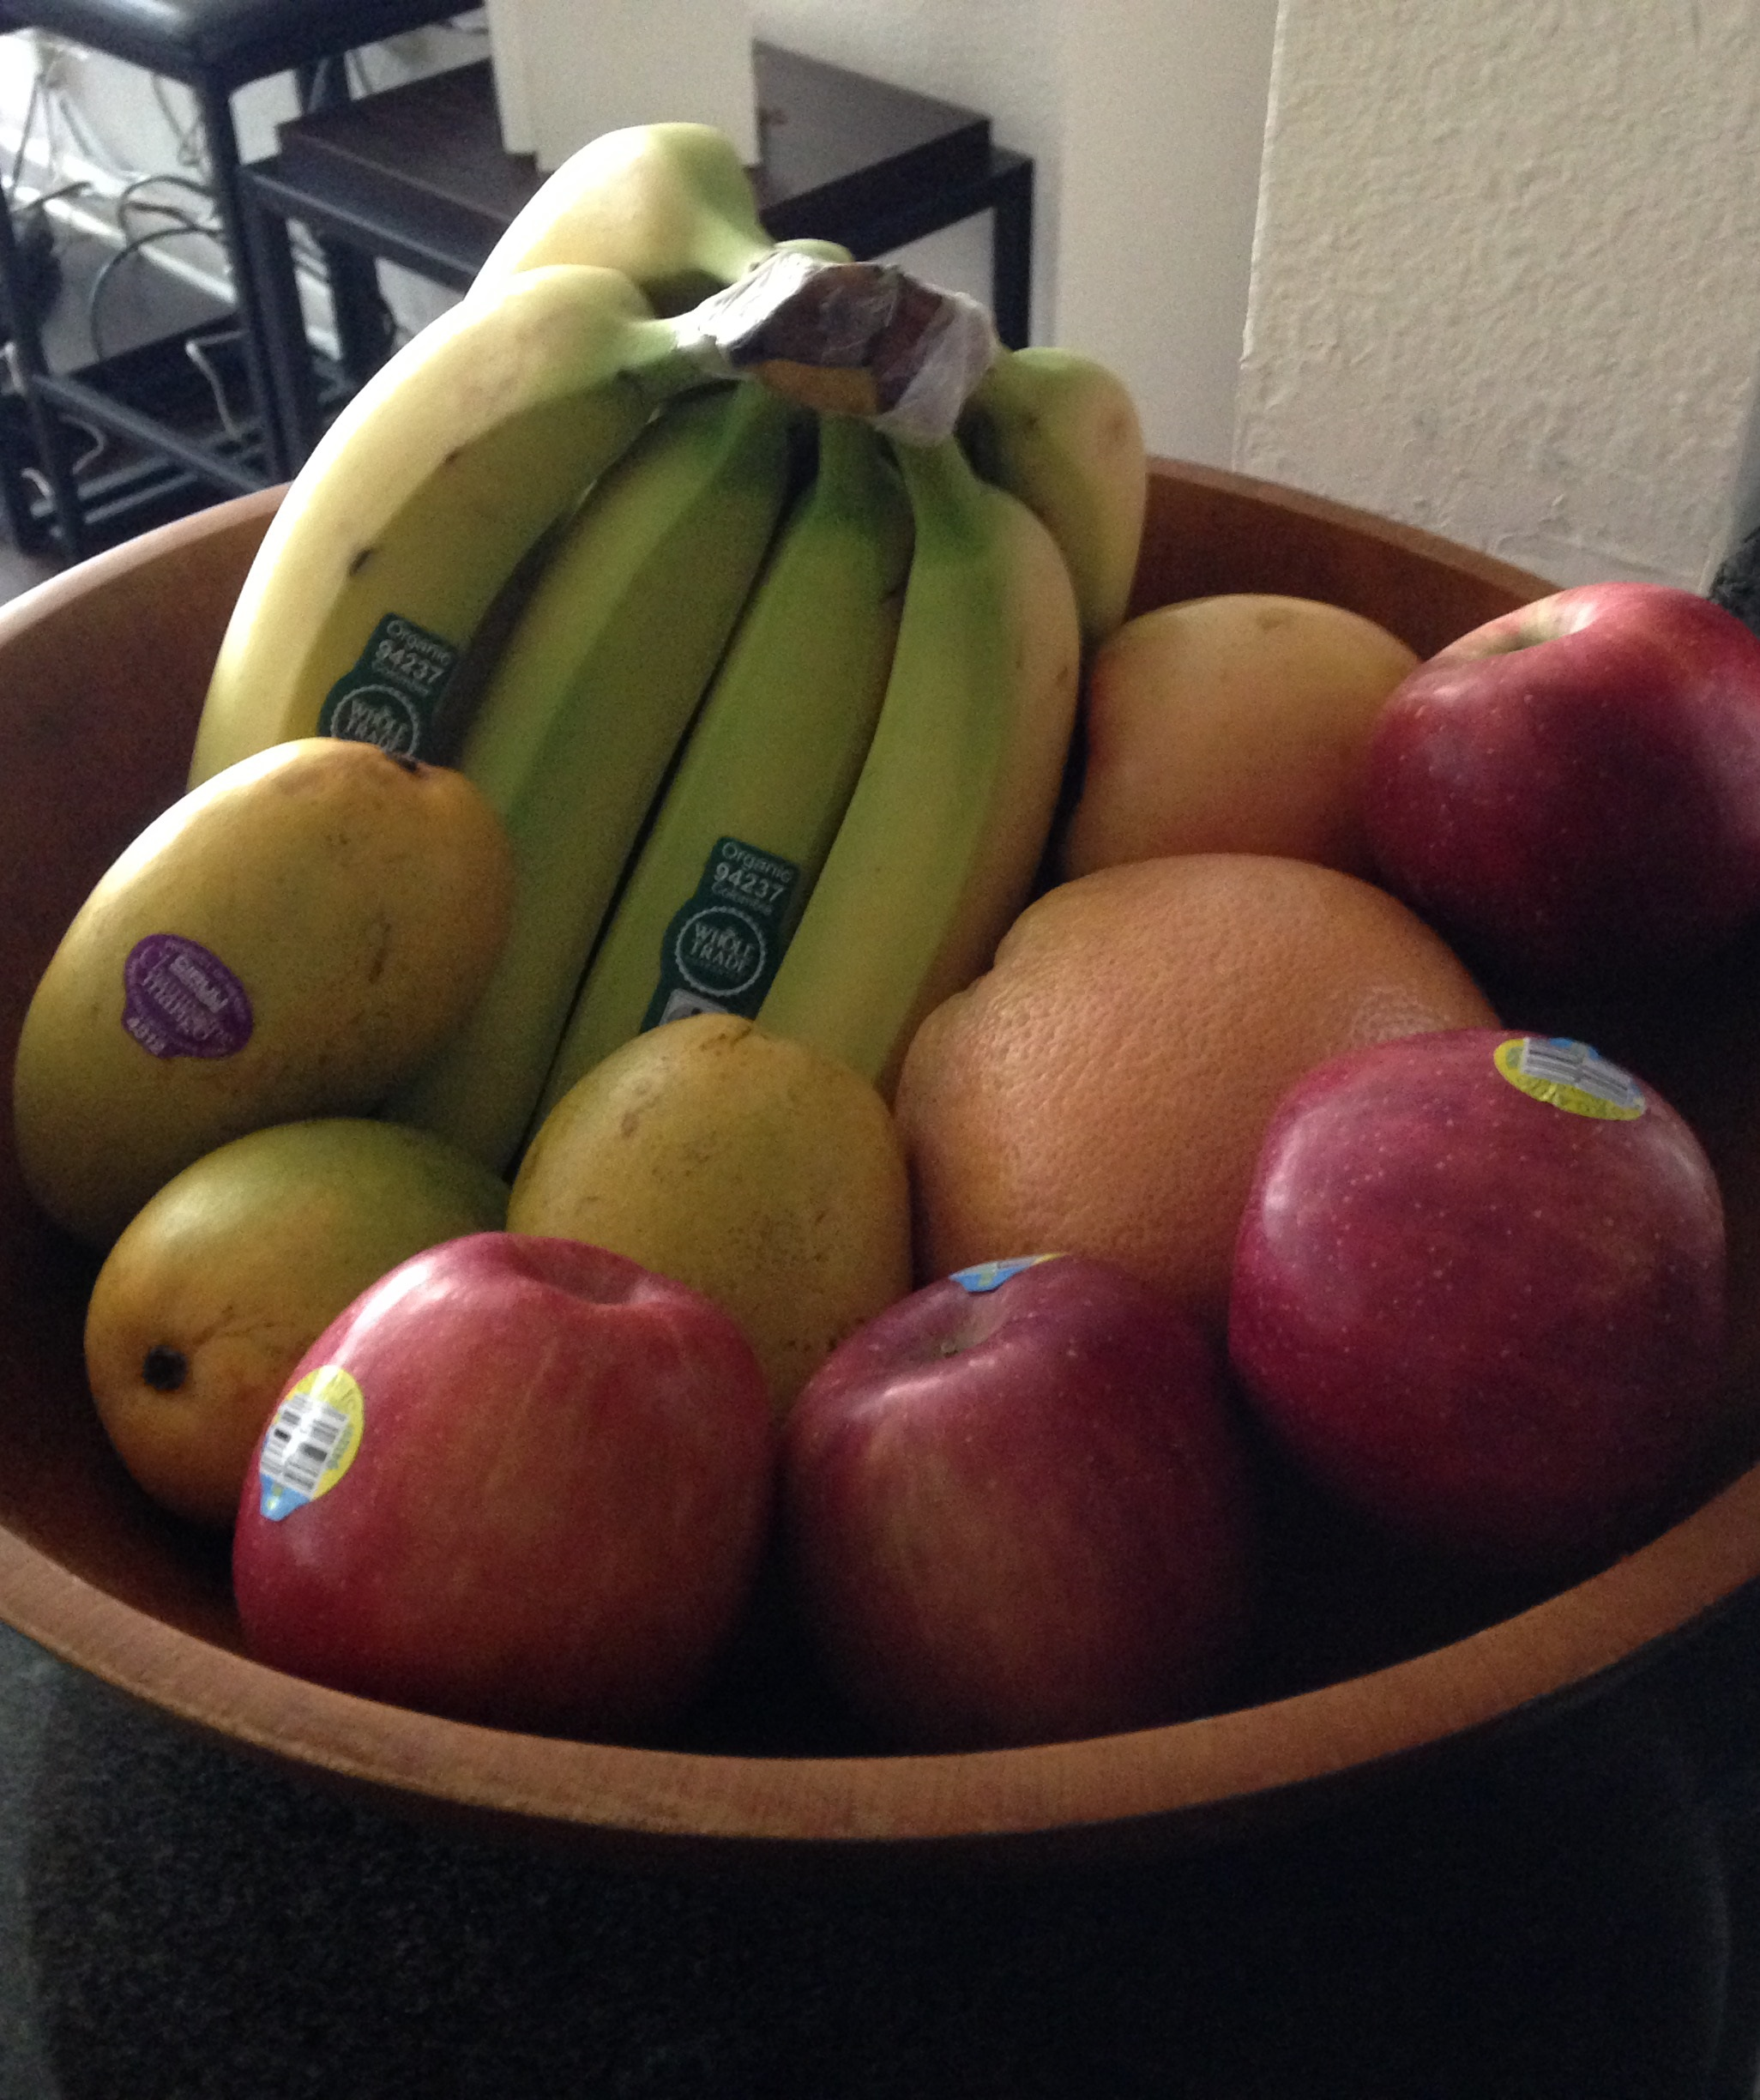
\includegraphics[height=\paperheight,
				keepaspectratio]{./Images/FruitBowl.jpg}}%
			\vfill
}}}

%STEAK
\newcommand\Steak{%
	\put(0,0){%
		\parbox[b][\paperheight]{\paperwidth}{%
			\vfill
			\centering
			{\transparent{0.3} 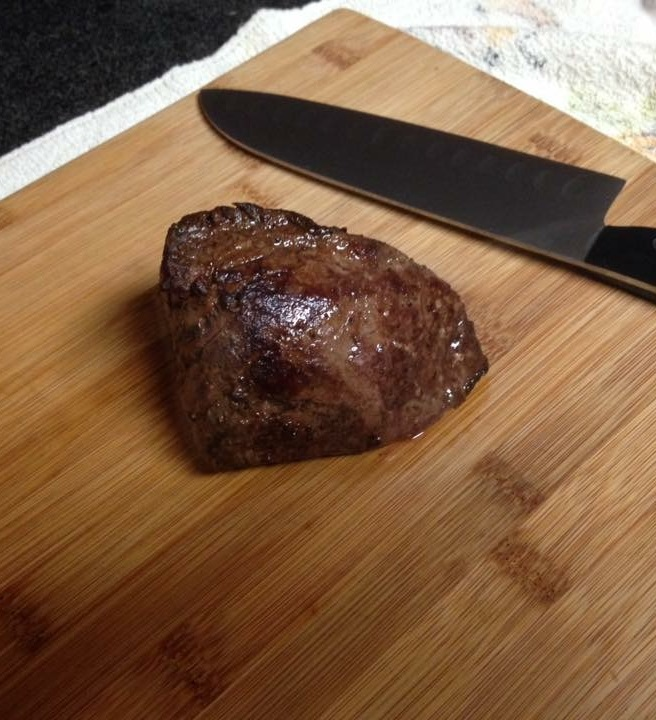
\includegraphics[height=\paperheight,
				keepaspectratio]{./Images/Steak.jpg}}%
			\vfill
}}}

%APPLETARTLARGE
\newcommand\AppleTartLarge{%
	\put(0,0){%
		\parbox[b][\paperheight]{\paperwidth}{%
			\vfill
			\centering
			{\transparent{0.3} 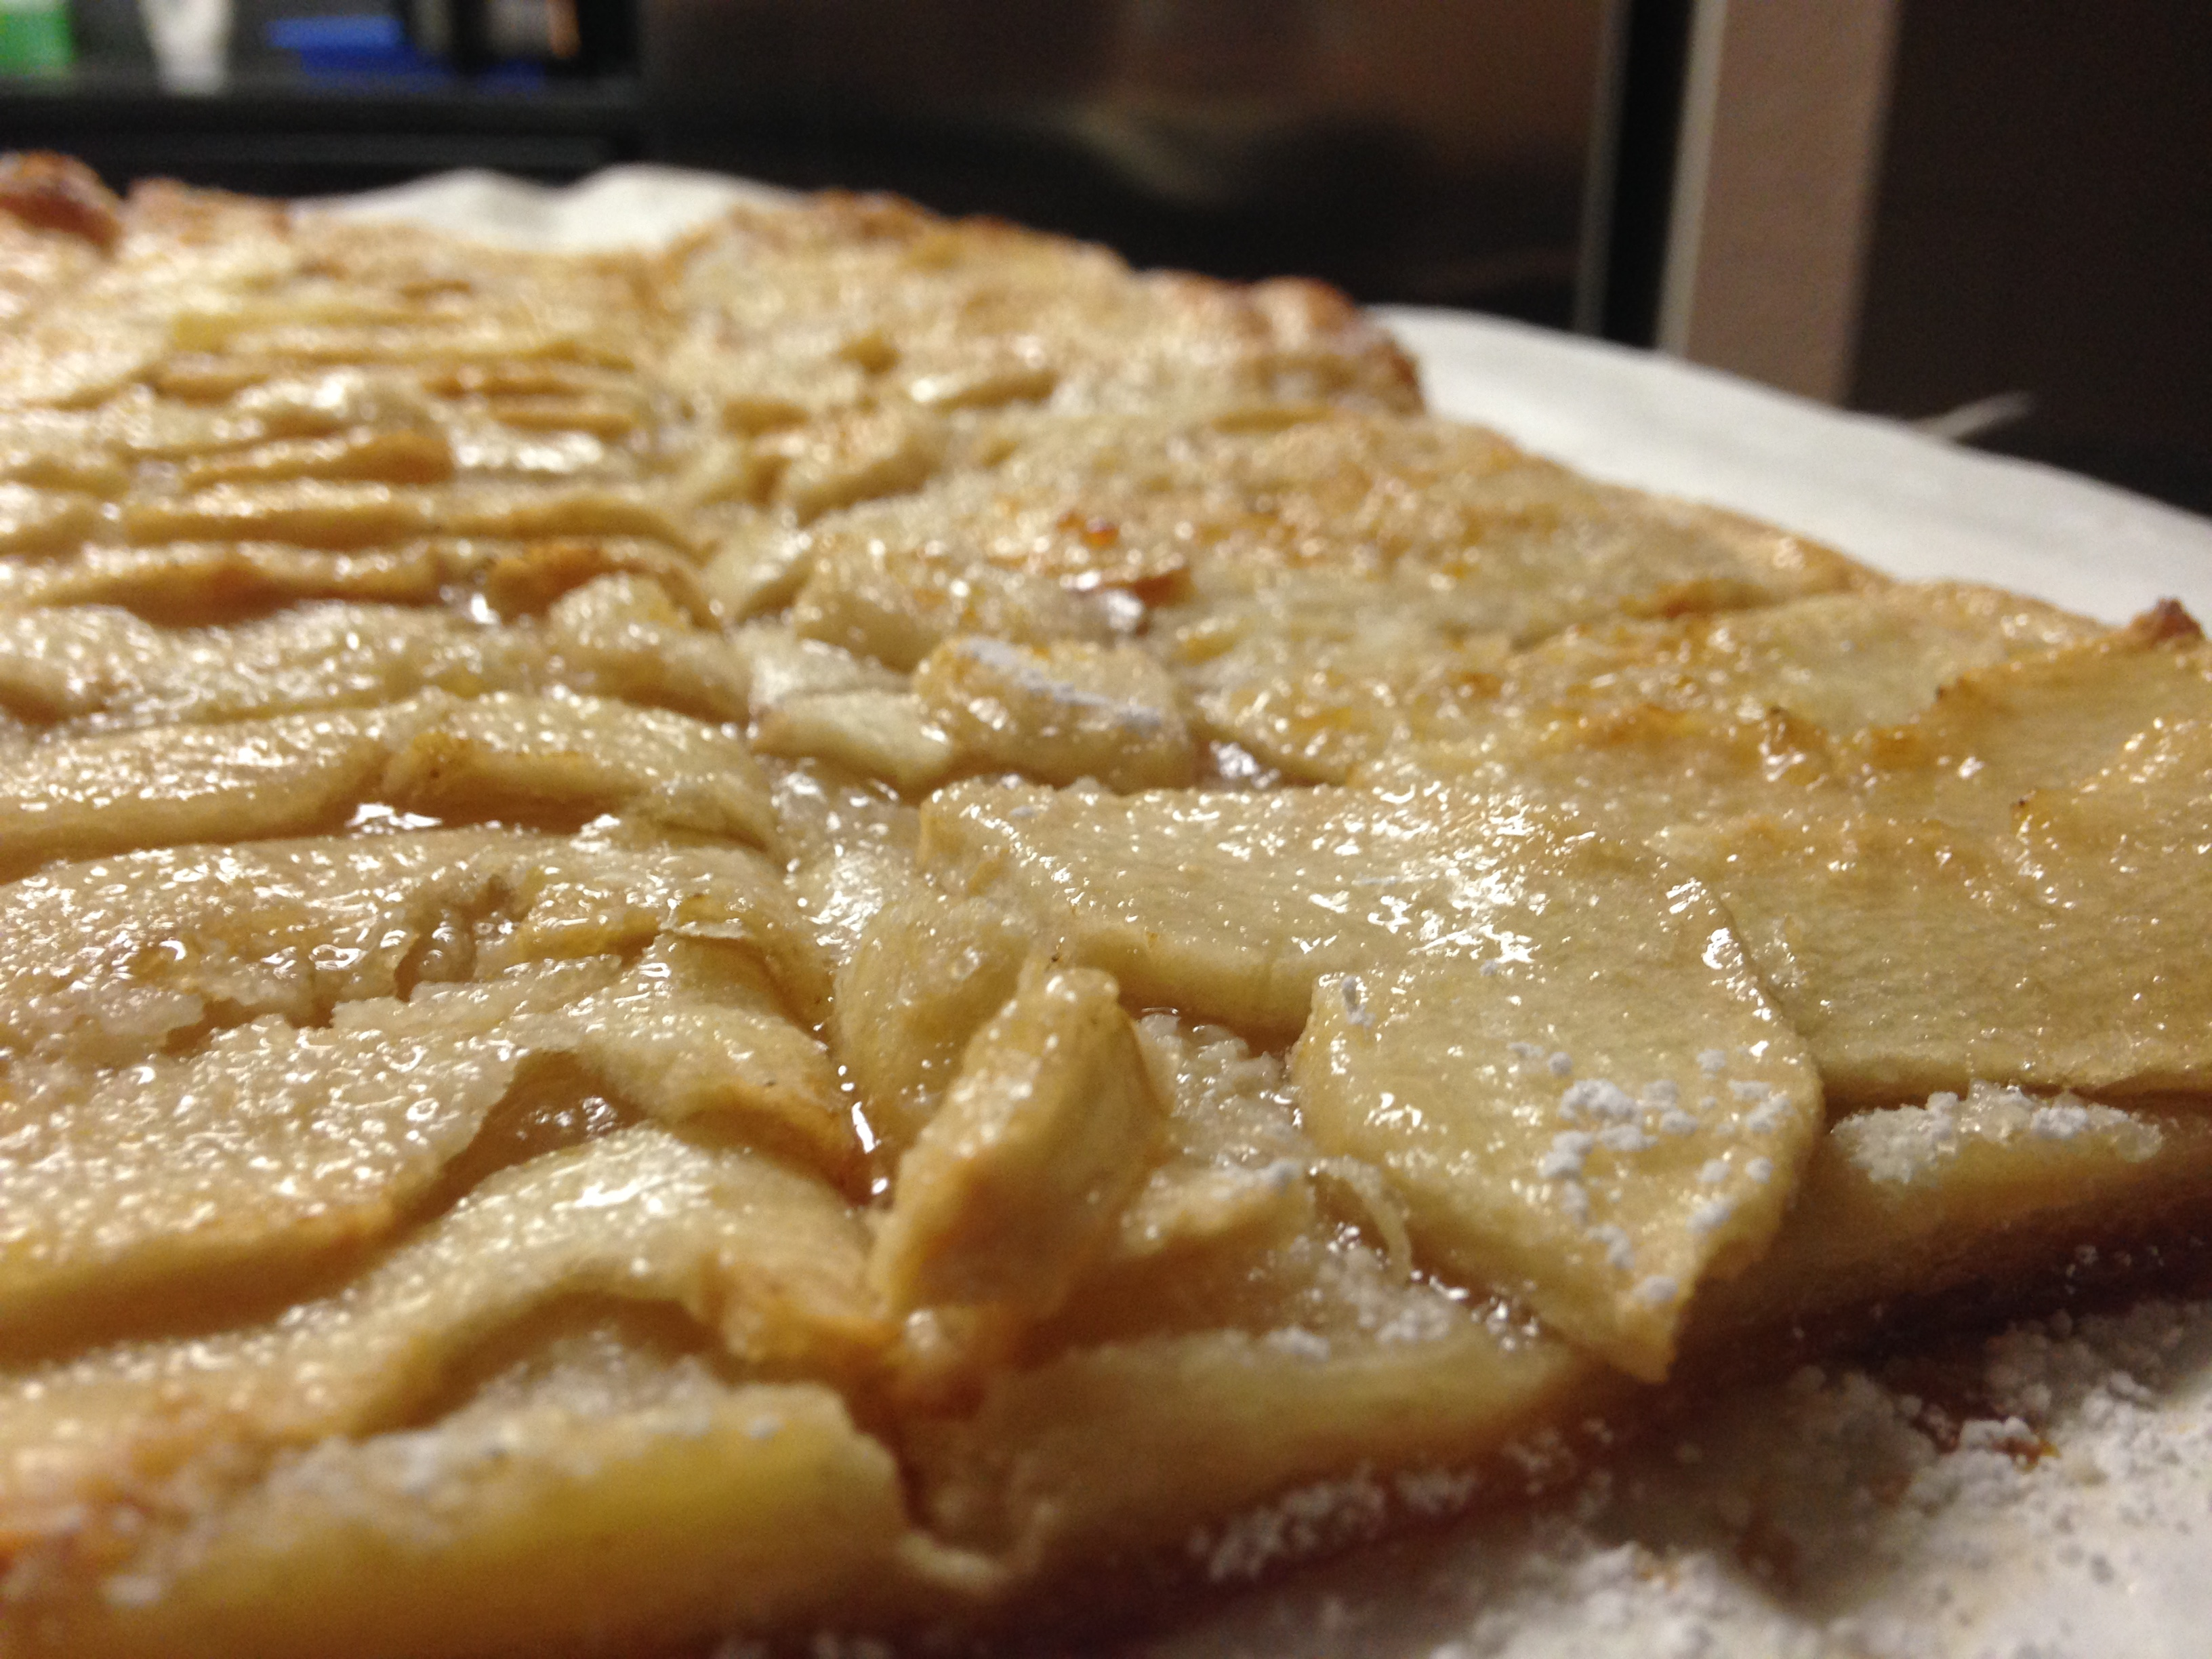
\includegraphics[height=\paperheight,
				keepaspectratio]{./Images/AppleTartLarge.jpg}}%
			\vfill
}}}

%STRAWBERRIES
\newcommand\Strawberries{%
	\put(0,0){%
		\parbox[b][\paperheight]{\paperwidth}{%
			\vfill
			\centering
			{\transparent{0.3} 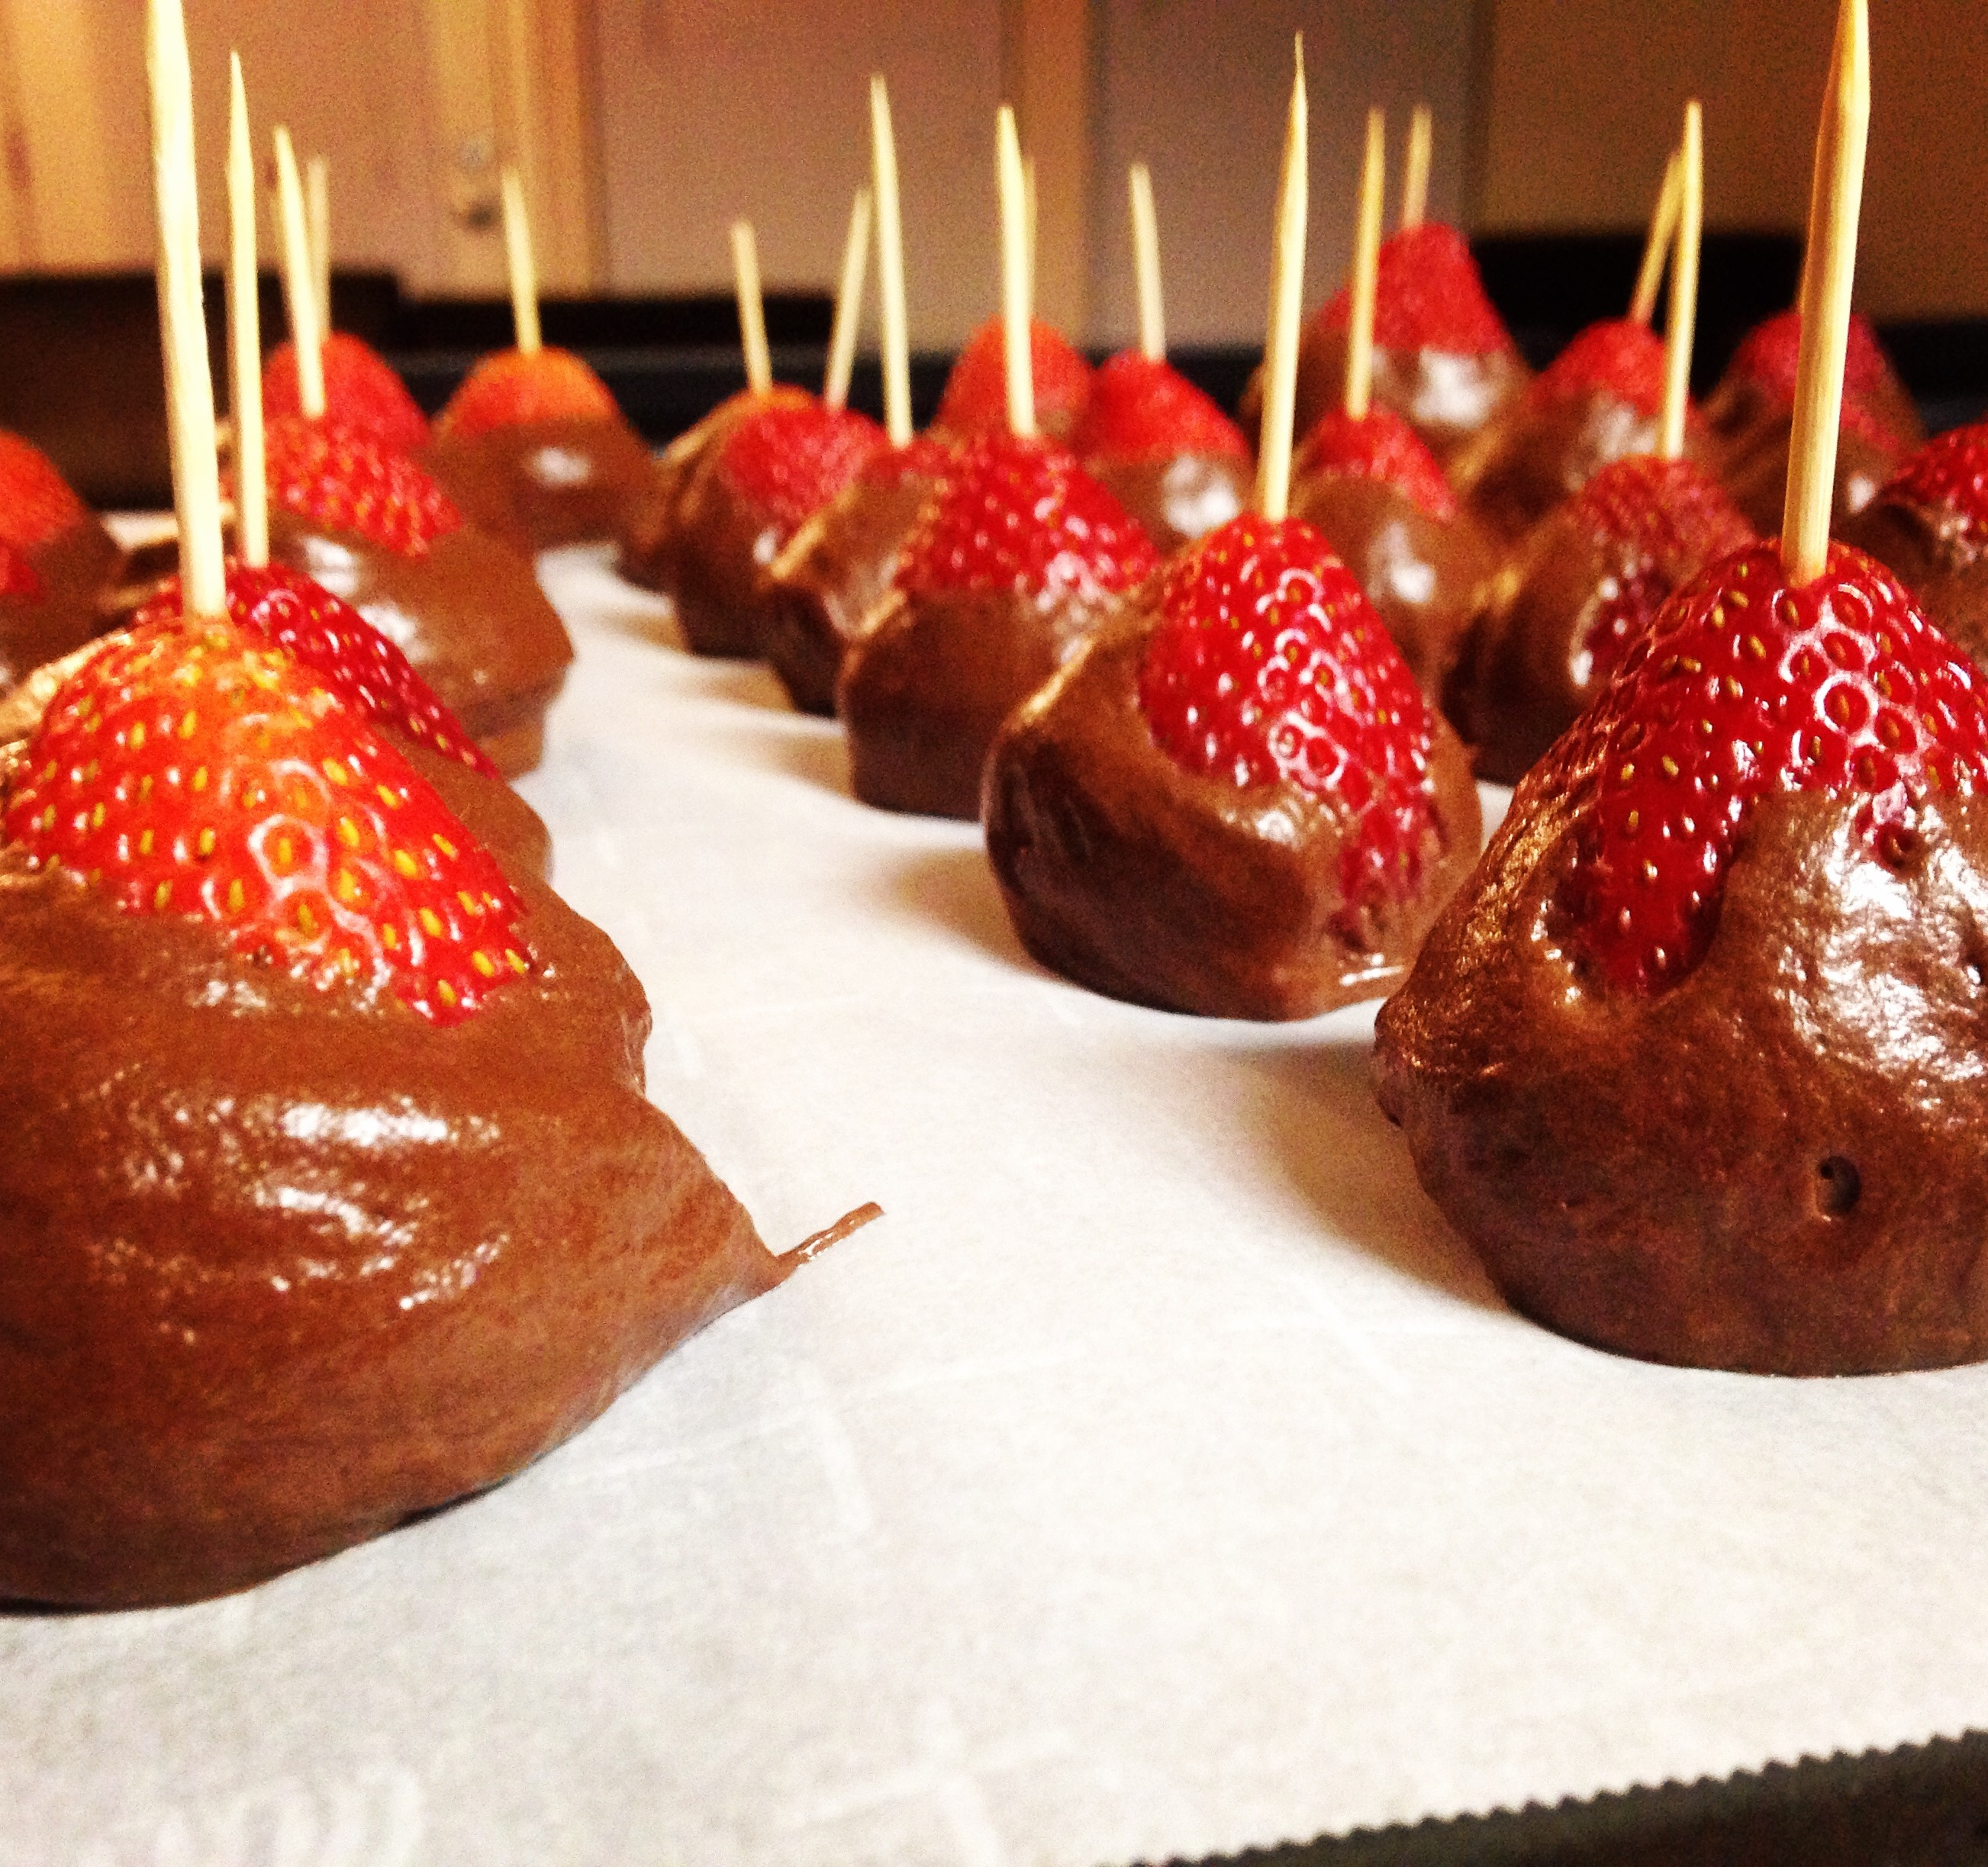
\includegraphics[height=\paperheight,%
				keepaspectratio]{./Images/Strawberries.jpg}}%
			\vfill
}}}

%SALMONVEGETABLERICE
\newcommand\SalmonVegetableRice{%
	\put(0,0){%
		\parbox[b][\paperheight]{\paperwidth}{%
			\vfill
			\centering
			{\transparent{0.3} 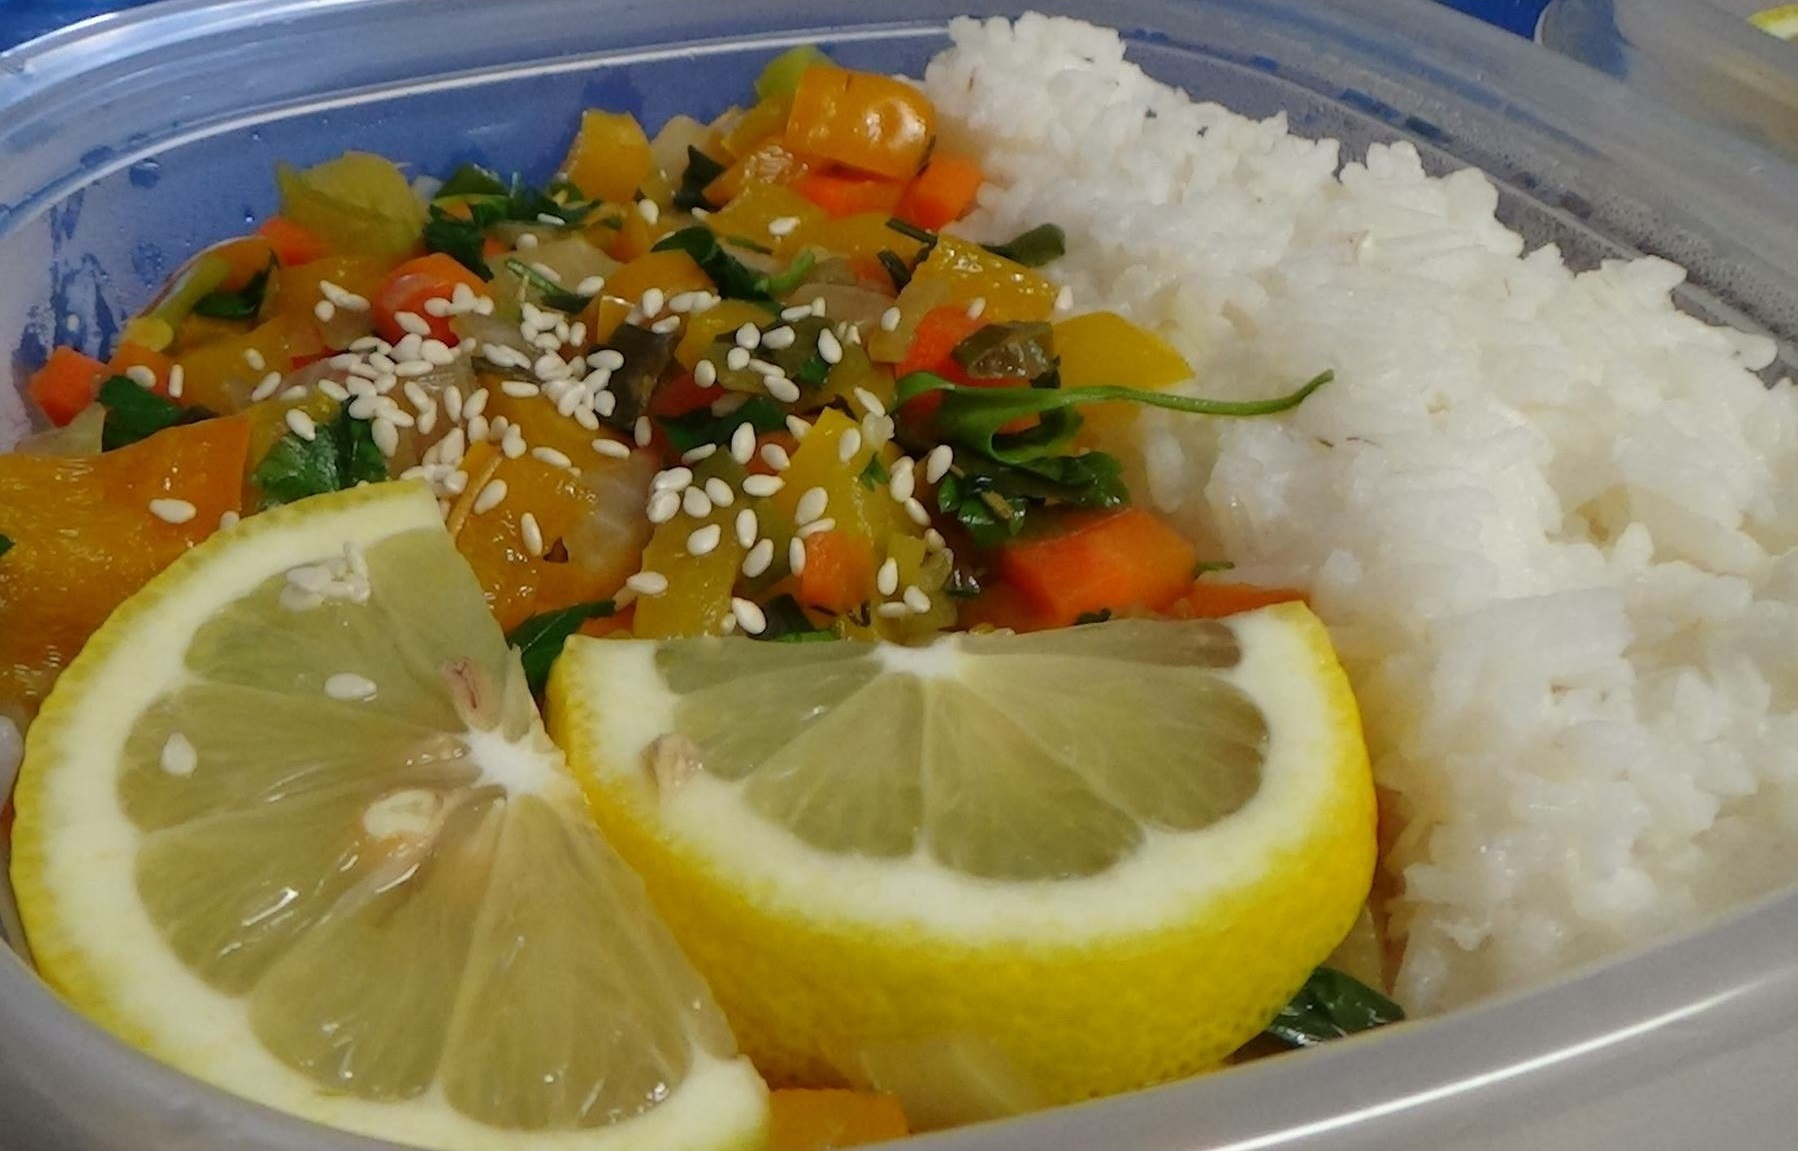
\includegraphics[height=\paperheight,%
				keepaspectratio]{./Images/SalmonVegetableRice.jpg}}%
			\vfill
}}}

%CHEESECAKE
\newcommand\Cheesecake{%
	\put(0,0){%
		\parbox[b][\paperheight]{\paperwidth}{%
			\vfill
			\centering
			{\transparent{0.3} 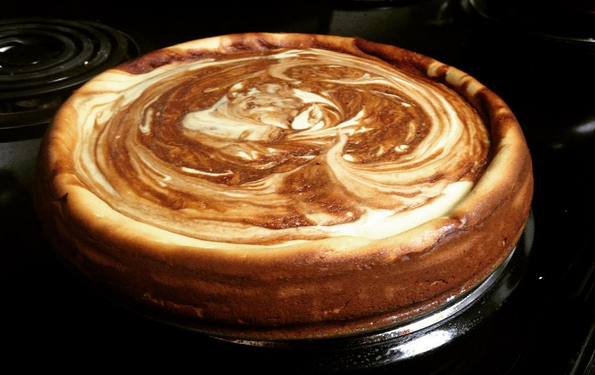
\includegraphics[height=\paperheight,%
				keepaspectratio]{./Images/MarbledCheesecake.png}}%
			\vfill
}}}

%CHICKENSALAD
\newcommand\ChickenSalad{%
	\put(0,0){%
		\parbox[b][\paperheight]{\paperwidth}{%
			\vfill
			\centering
			{\transparent{0.3} 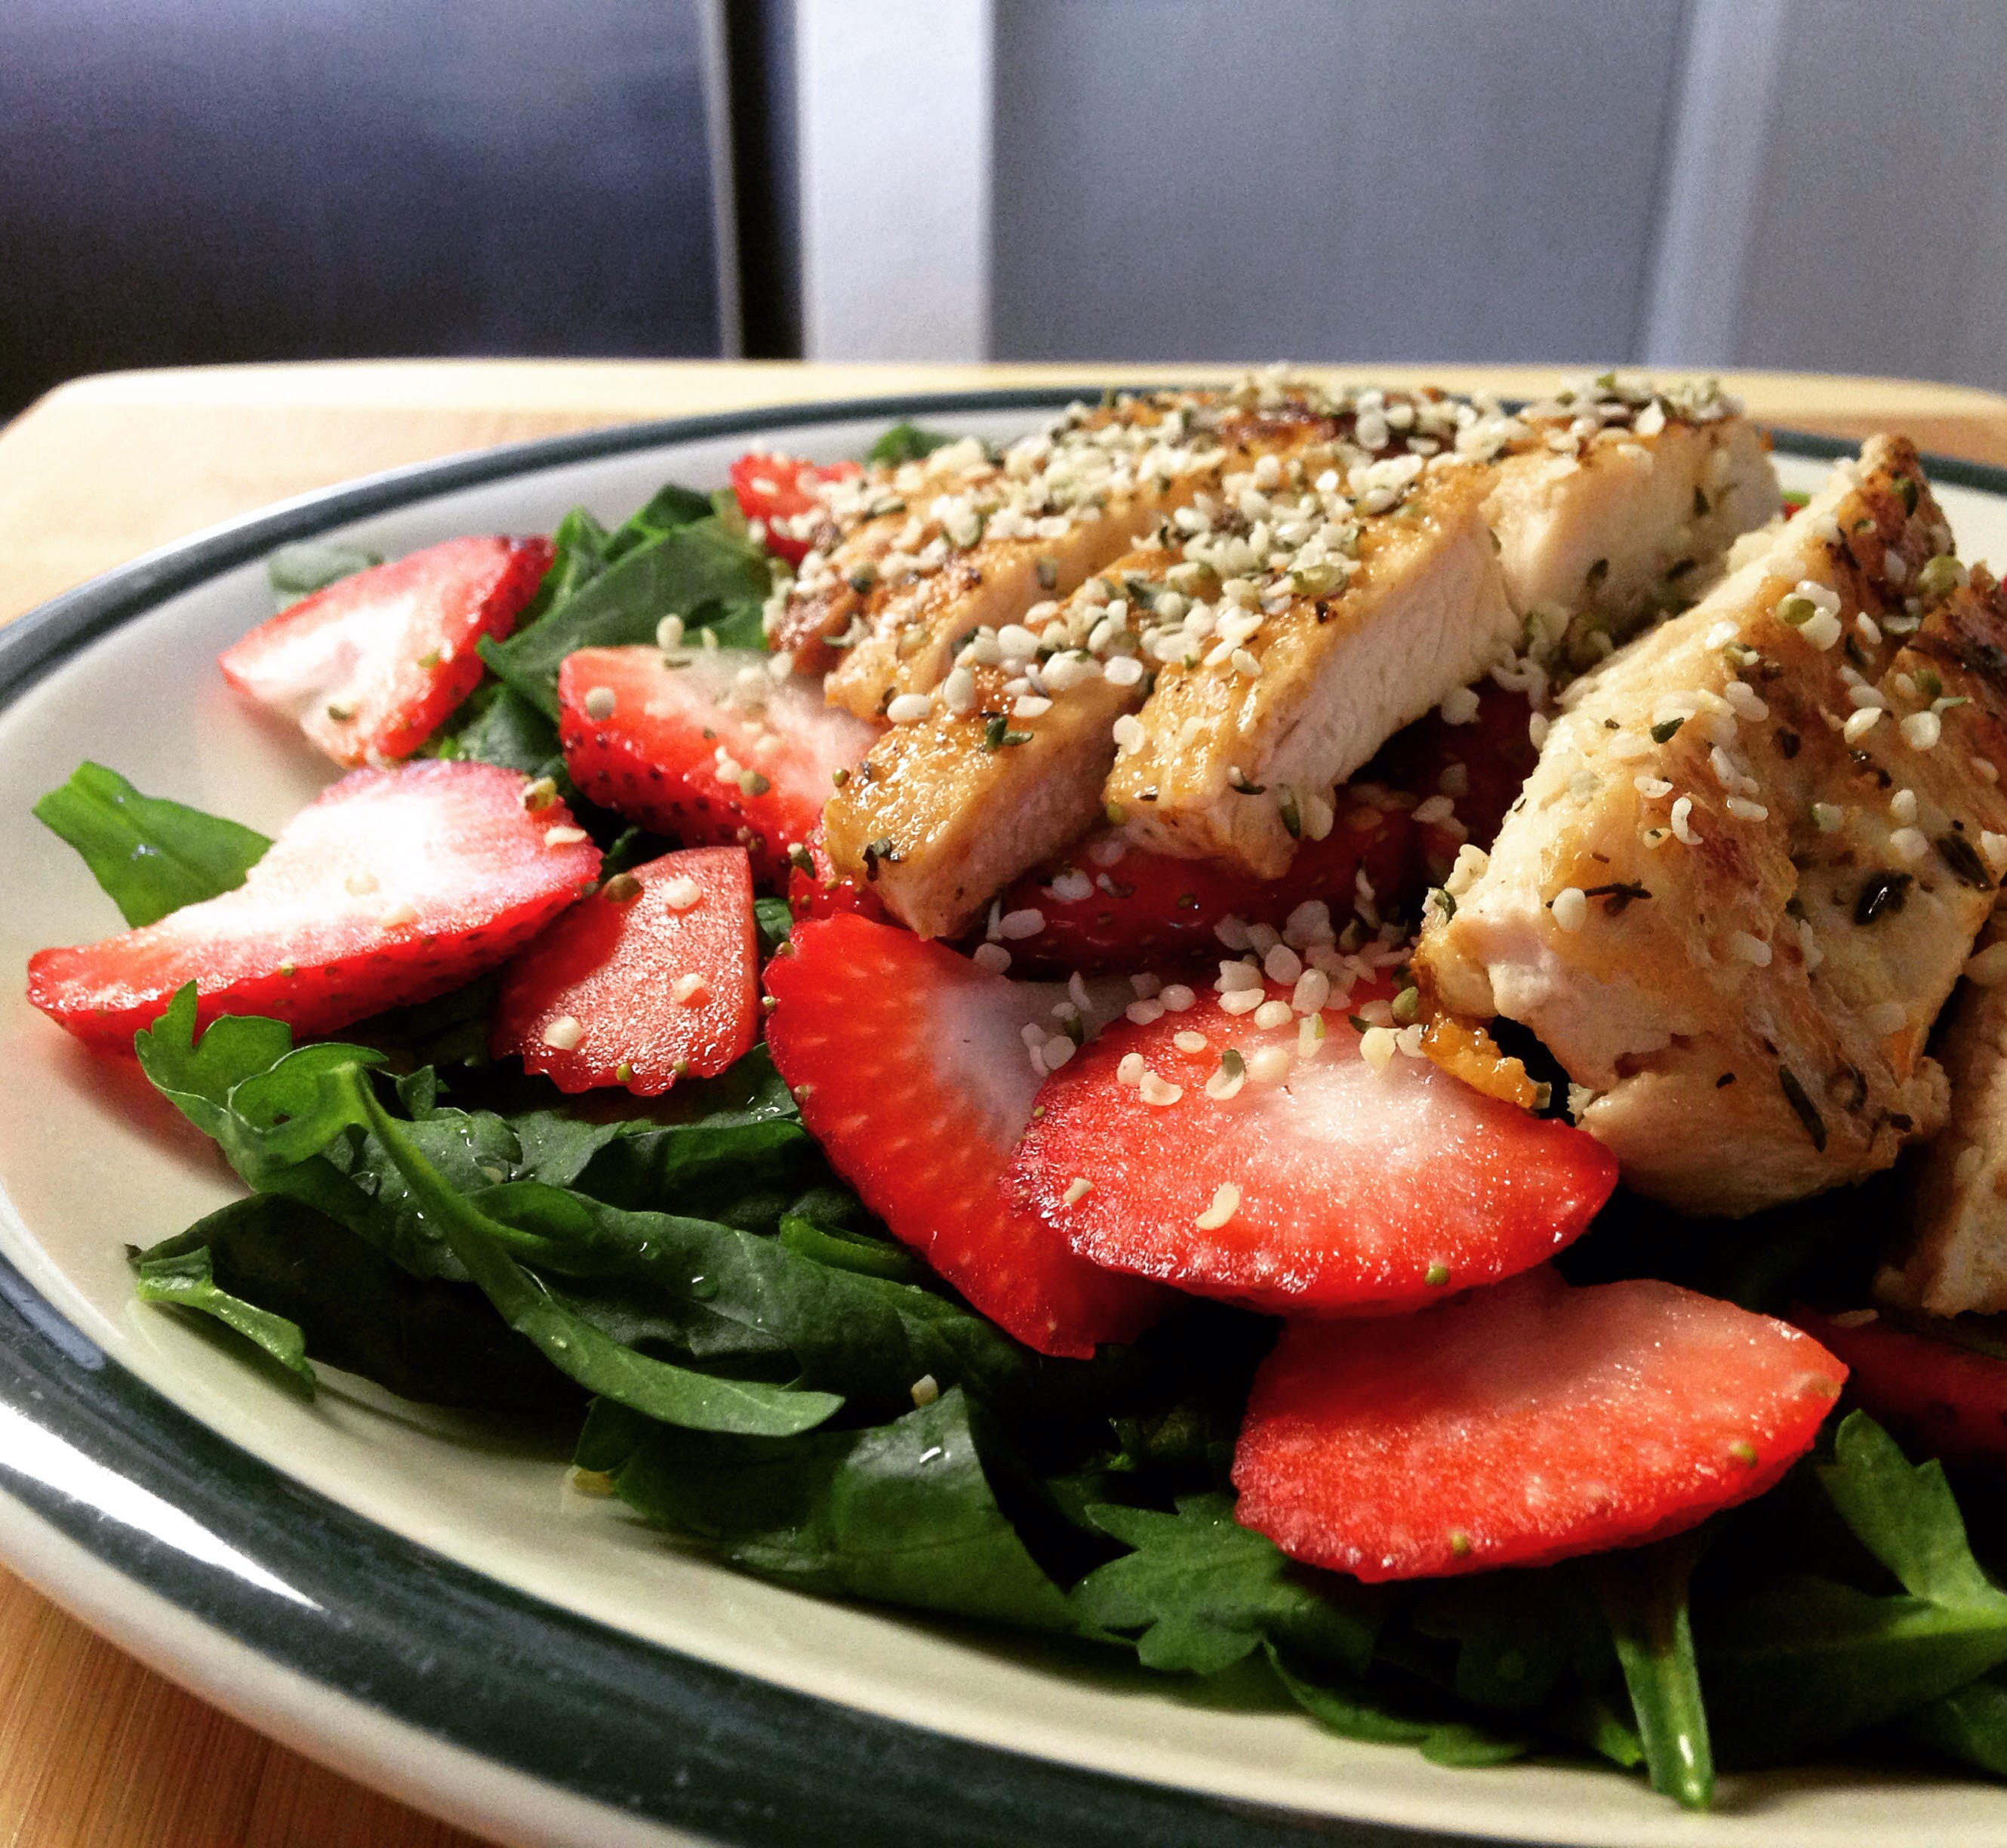
\includegraphics[height=\paperheight,%
				keepaspectratio]{./Images/ChickenSalad.jpg}}%
			\vfill
}}}

%MEXICANSOUP
\newcommand\MexicanSoup{%
	\put(0,0){%
		\parbox[b][\paperheight]{\paperwidth}{%
			\vfill
			\centering
			{\transparent{0.3} 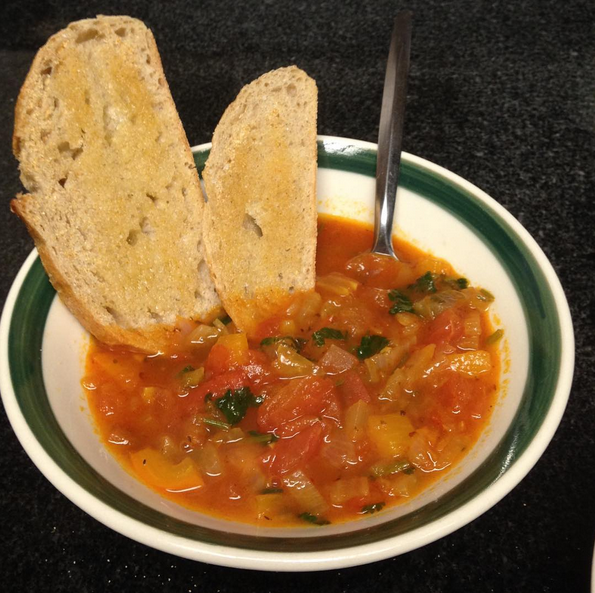
\includegraphics[height=\paperheight,%
				keepaspectratio]{./Images/SpicyMexicanSoup.png}}%
			\vfill
}}}

%CALZONE
\newcommand\Calzone{%
	\put(0,0){%
		\parbox[b][\paperheight]{\paperwidth}{%
			\vfill
			\centering
			{\transparent{0.3} 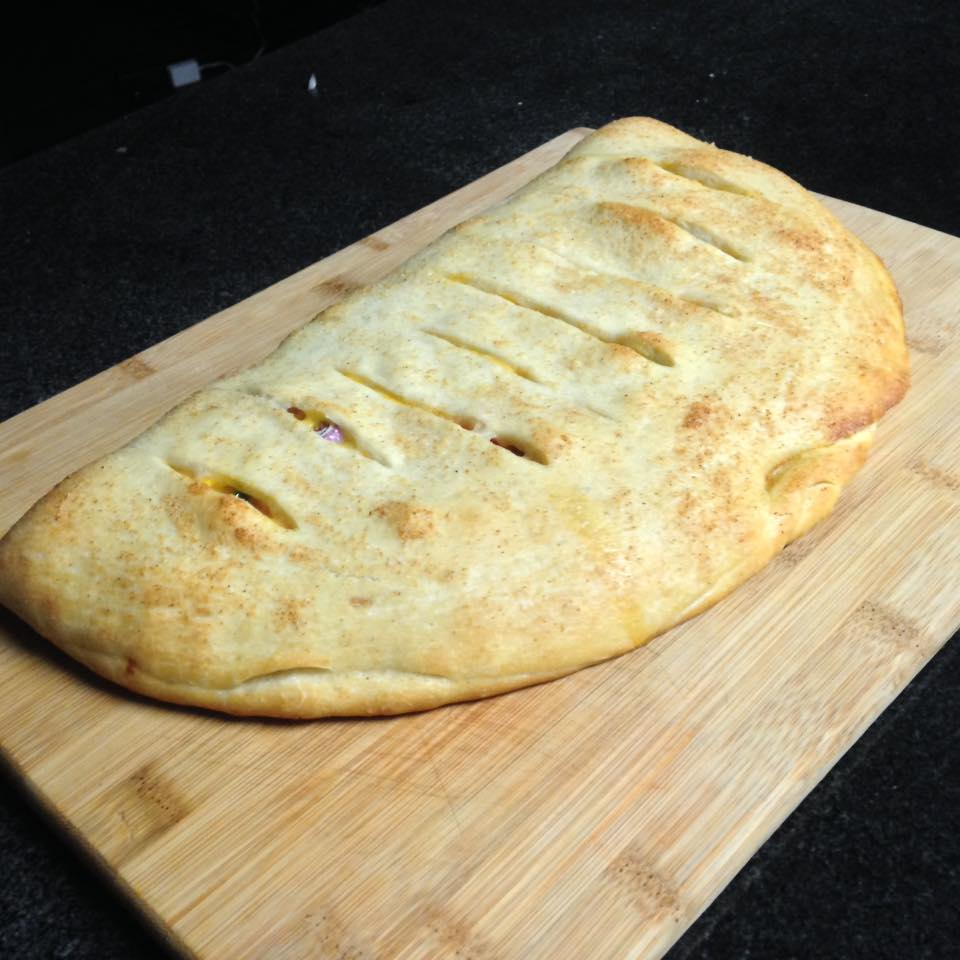
\includegraphics[height=\paperheight,%
				keepaspectratio]{./Images/Calzone.jpg}}%
			\vfill
}}}

%CHEESECAKETOPPING
\newcommand\CheesecakeTopping{%
	\put(0,0){%
		\parbox[b][\paperheight]{\paperwidth}{%
			\vfill
			\centering
			{\transparent{0.3} 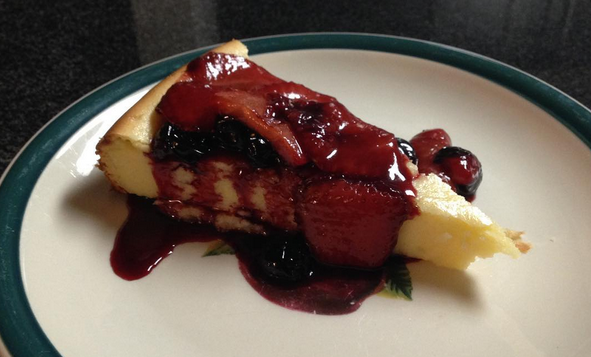
\includegraphics[height=\paperheight,%
				keepaspectratio]{./Images/CheesecakeTopping.png}}%
			\vfill
}}}

%MANGOSALSATACO
\newcommand\MangoSalsaTaco{%
	\put(0,0){%
		\parbox[b][\paperheight]{\paperwidth}{%
			\vfill
			\centering
			{\transparent{0.3} 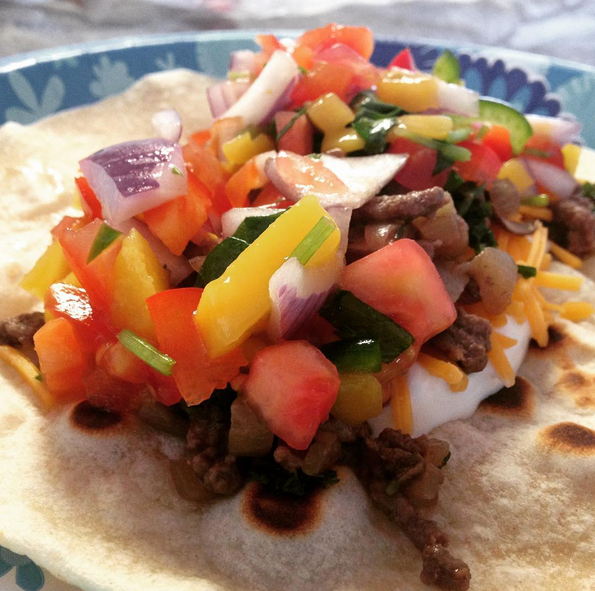
\includegraphics[height=\paperheight,%
				keepaspectratio]{./Images/MangeSalsaTacos.png}}%
			\vfill
}}}

%EGGSANDWICH
\newcommand\EggSandwich{%
	\put(0,0){%
		\parbox[b][\paperheight]{\paperwidth}{%
			\vfill
			\centering
			{\transparent{0.3} 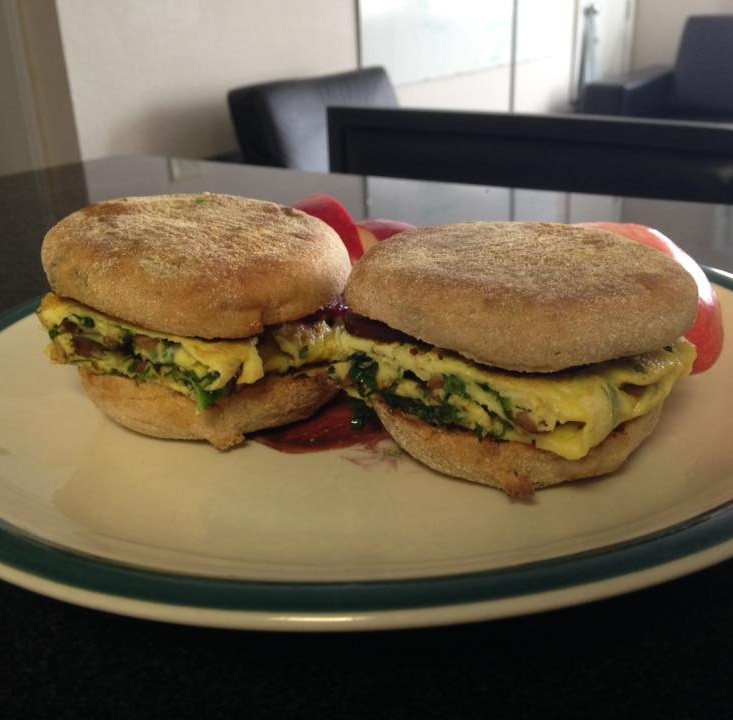
\includegraphics[height=\paperheight,%
				keepaspectratio]{./Images/EggSandwich.jpg}}%
			\vfill
}}}

%APPLETART
\newcommand\AppleTart{%
	\put(0,0){%
		\parbox[b][\paperheight]{\paperwidth}{%
			\vfill
			\centering
			{\transparent{0.3} 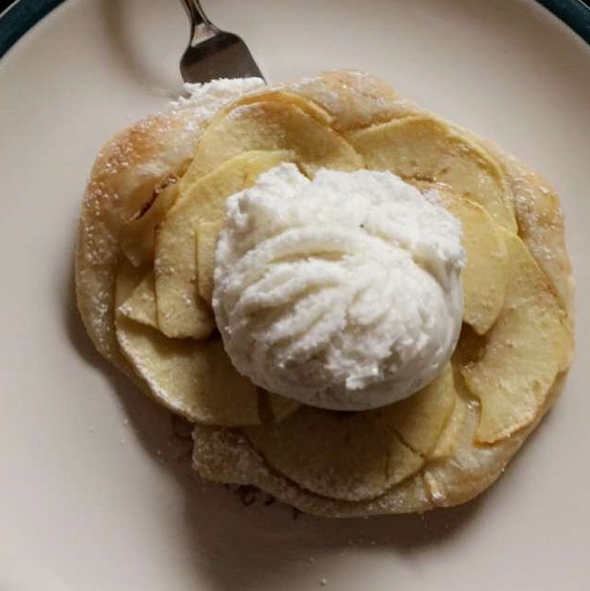
\includegraphics[height=\paperheight,%
				keepaspectratio]{./Images/AppleTartDesert.png}}%
			\vfill
}}}

%MARINATEDCHICKENANDRICE
\newcommand\MarinatedChickenAndRice{%
	\put(0,0){%
		\parbox[b][\paperheight]{\paperwidth}{%
			\vfill
			\centering
			{\transparent{0.3} 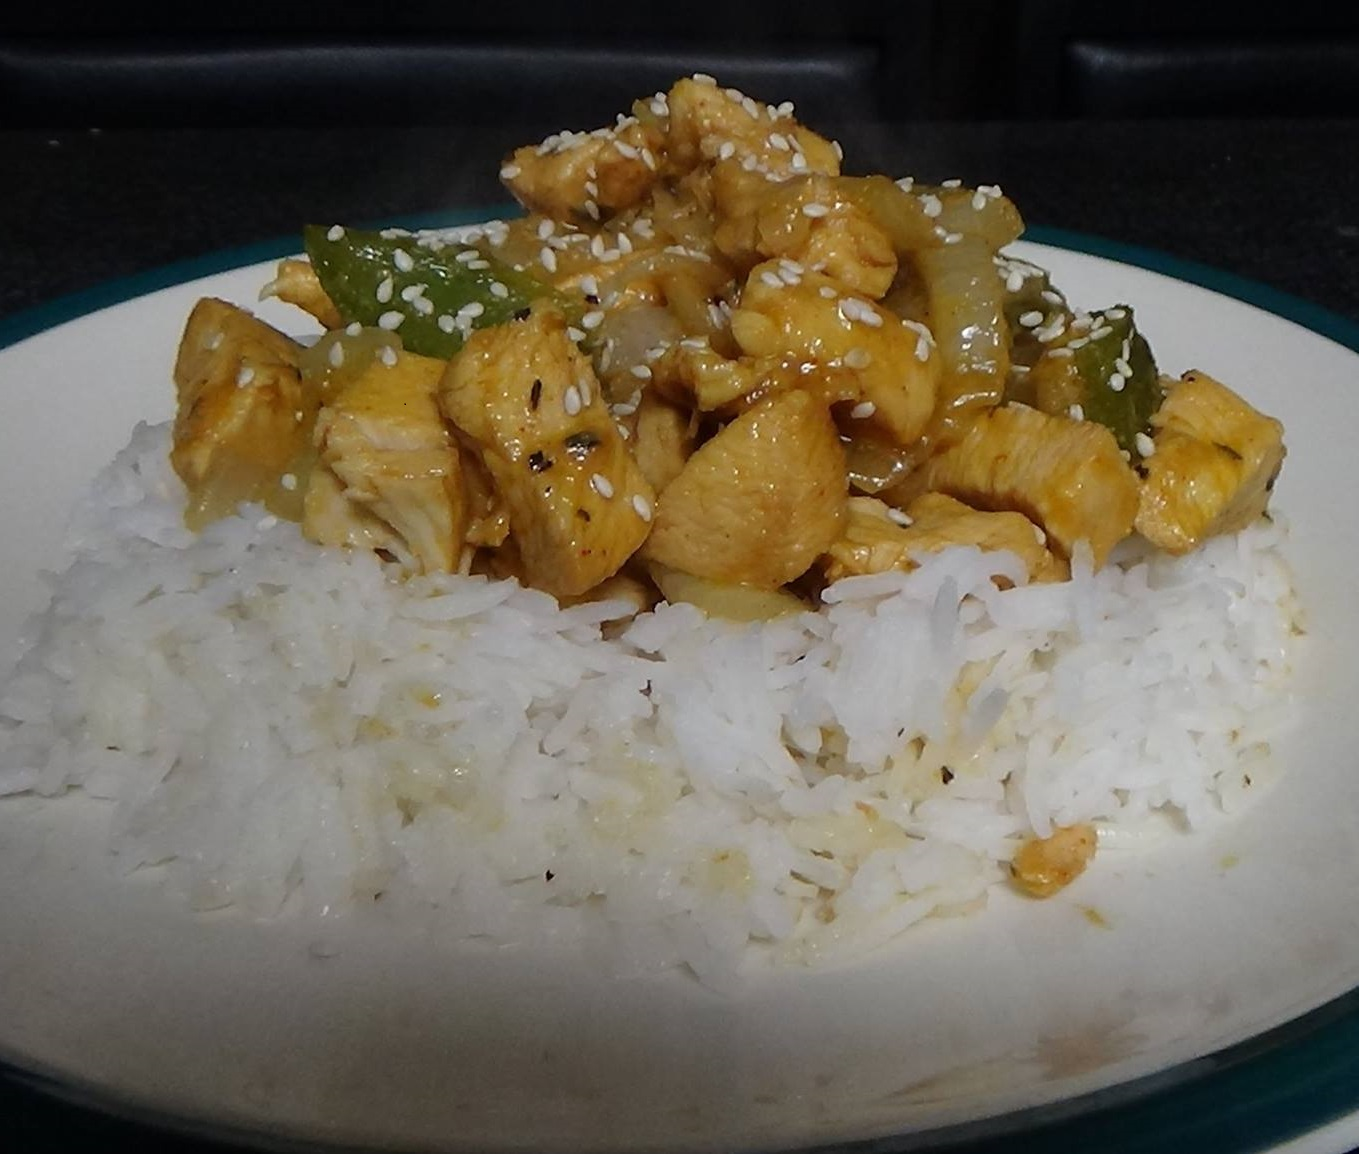
\includegraphics[height=\paperheight,%
				keepaspectratio]{./Images/chickenveggiesrice.jpg}}%
			\vfill
}}}

%FETASPINACHEGGS
\newcommand\FetaSpinachEggs{%
	\put(0,0){%
		\parbox[b][\paperheight]{\paperwidth}{%
			\vfill
			\centering
			{\transparent{0.3} 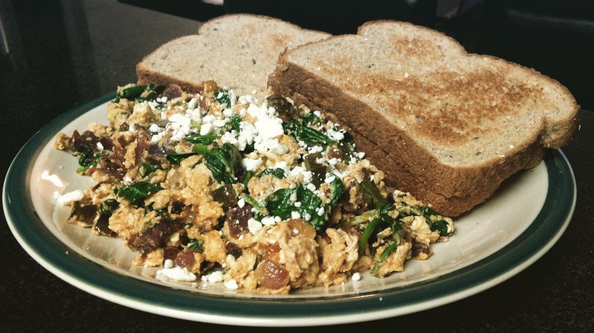
\includegraphics[height=\paperheight,%
				keepaspectratio]{./Images/FetaAndSpinachScrambledEggs.png}}%
			\vfill
}}}

%STIRFRYRICENOODLES
\newcommand\StirFryRiceNoodles{%
	\put(0,0){%
		\parbox[b][\paperheight]{\paperwidth}{%
			\vfill
			\centering
			{\transparent{0.3} 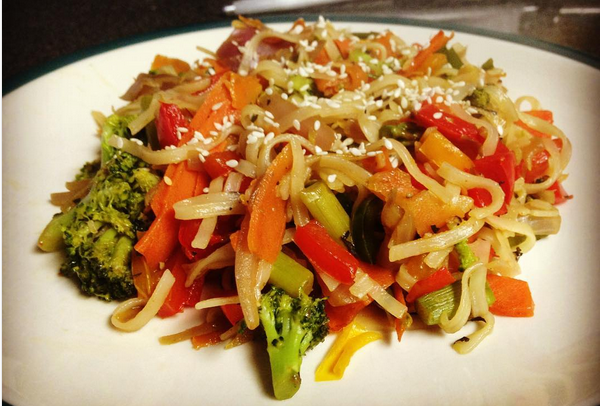
\includegraphics[height=\paperheight,%
				keepaspectratio]{./Images/StirFry_RiceNoodles.png}}%
			\vfill
}}}

%ALFREDO
\newcommand\Alfredo{%
	\put(0,0){%
		\parbox[b][\paperheight]{\paperwidth}{%
			\vfill
			\centering
			{\transparent{0.3} 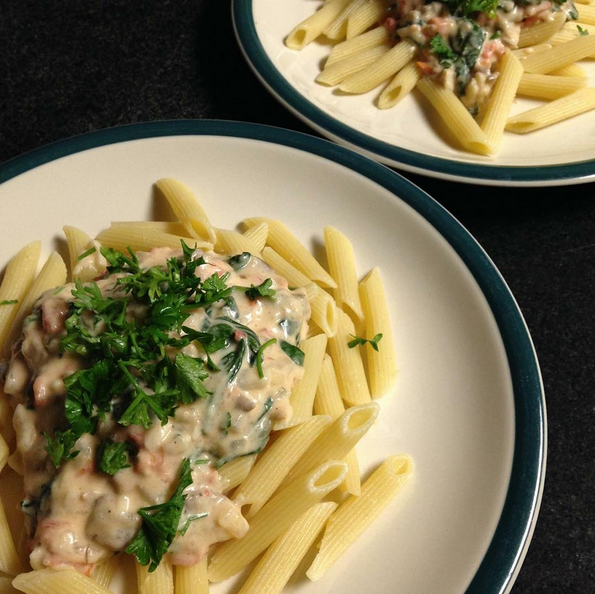
\includegraphics[height=\paperheight,%
				keepaspectratio]{./Images/Alfredo.png}}%
			\vfill
}}}

%STEAKANDEGGS
\newcommand\SteakAndEggs{%
	\put(0,0){%
		\parbox[b][\paperheight]{\paperwidth}{%
			\vfill
			\centering
			{\transparent{0.3} 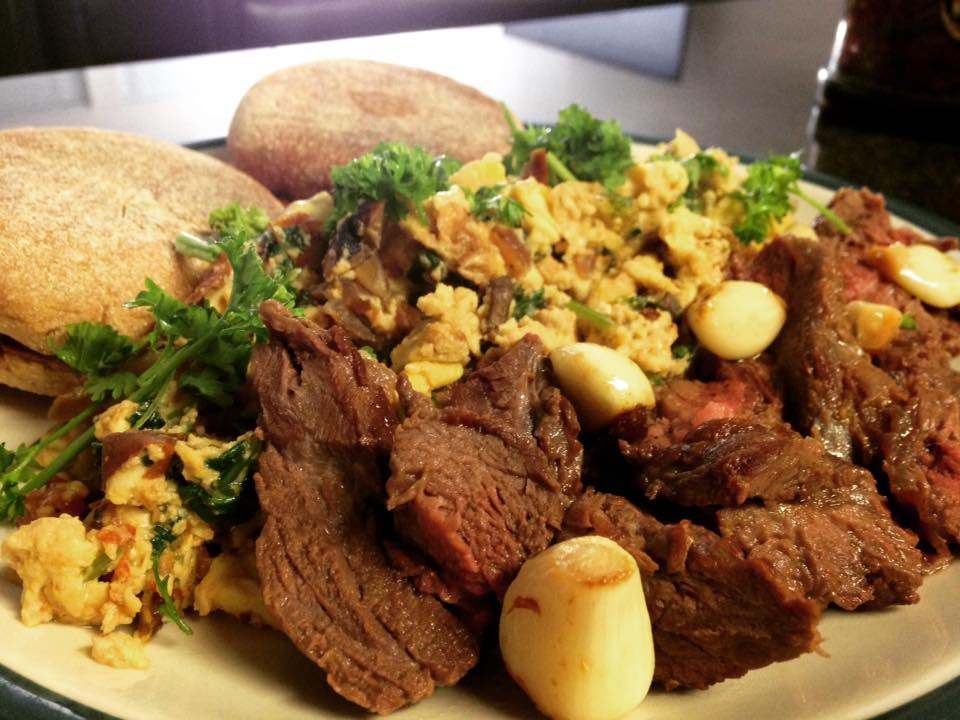
\includegraphics[height=\paperheight,%
				keepaspectratio]{./Images/SteakAndEggs.jpg}}%
			\vfill
}}}

%STEAKSANDWICH
\newcommand\SteakSandwich{%
	\put(0,0){%
		\parbox[b][\paperheight]{\paperwidth}{%
			\vfill
			\centering
			{\transparent{0.3} 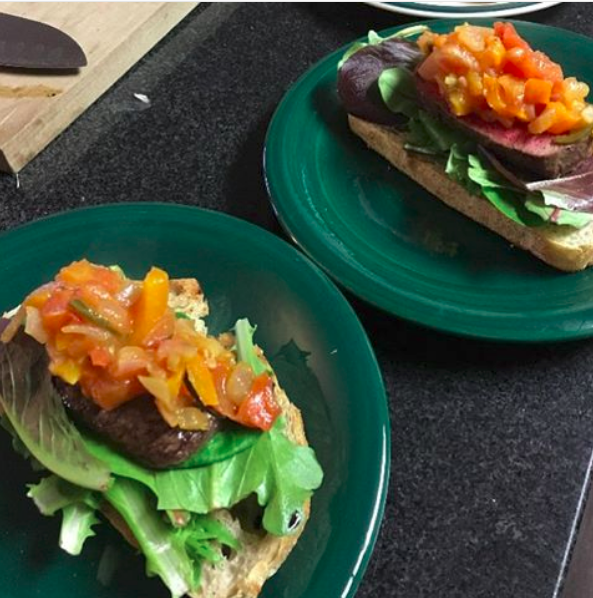
\includegraphics[height=\paperheight,%
				keepaspectratio]{./Images/SteakSandwich.png}}%
			\vfill
}}}

%PIZZA
\newcommand\Pizza{%
	\put(0,0){%
		\parbox[b][\paperheight]{\paperwidth}{%
			\vfill
			\centering
			{\transparent{0.3} 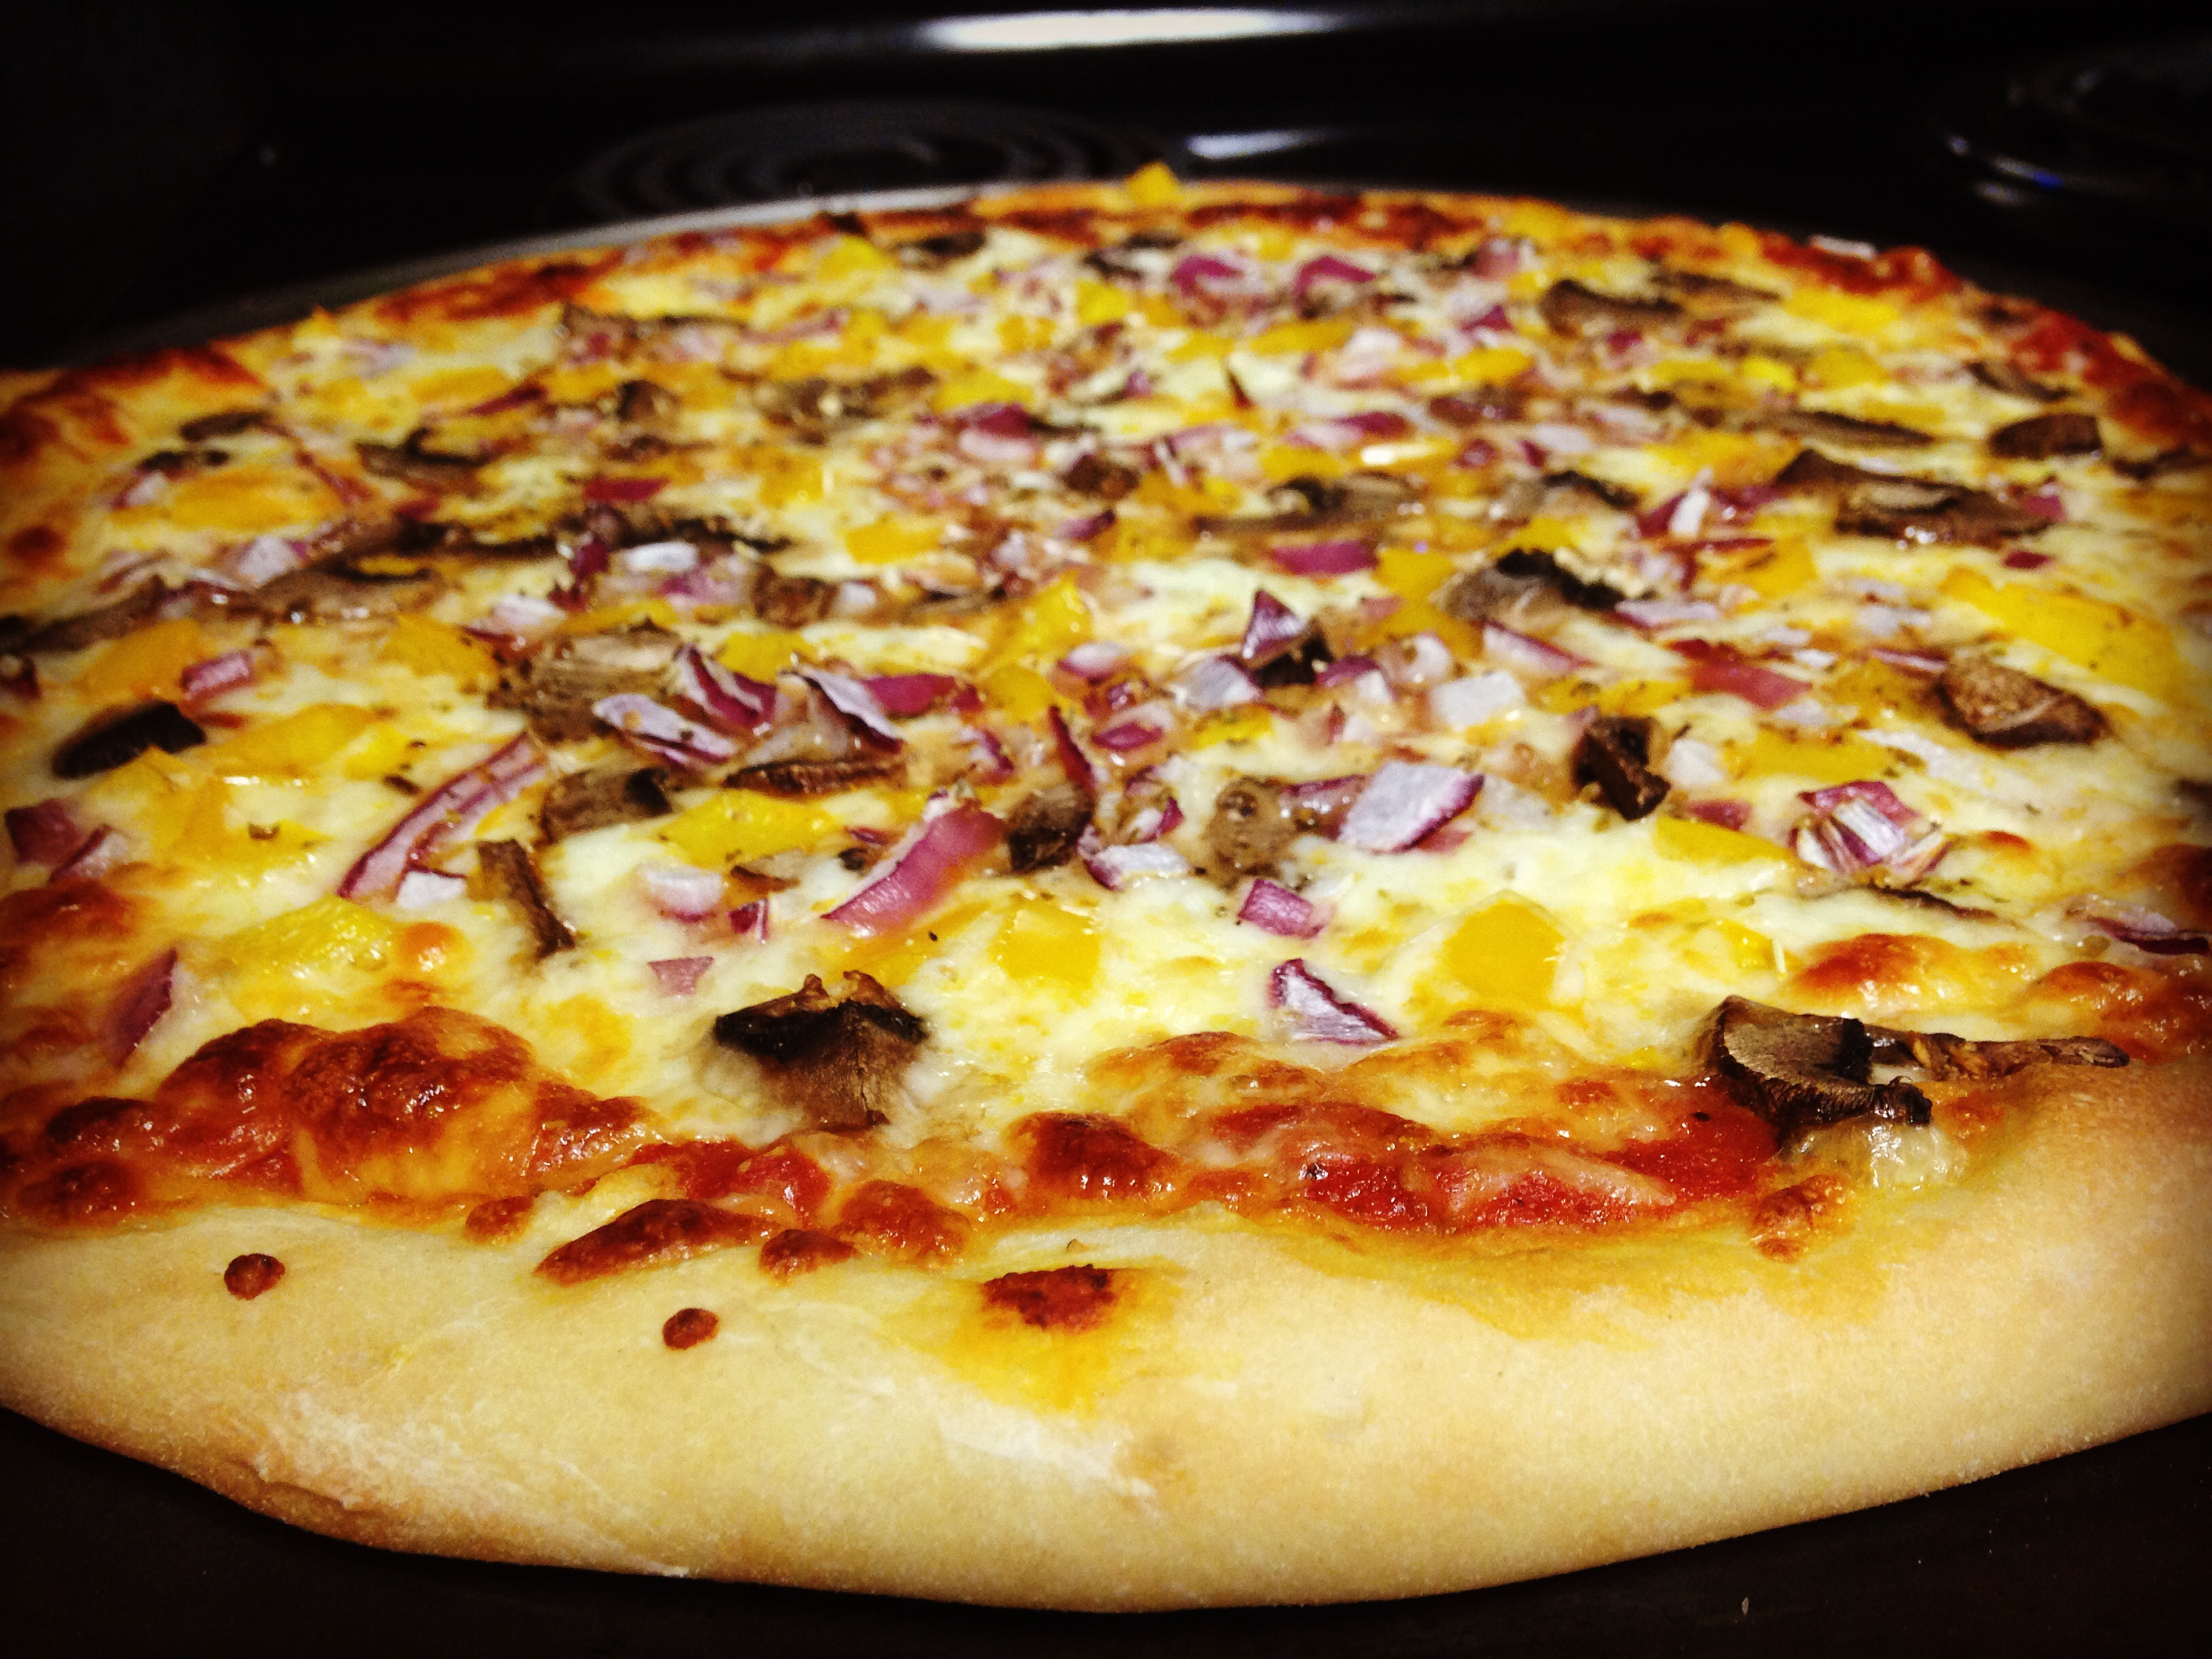
\includegraphics[height=\paperheight,%
				keepaspectratio]{./Images/Pizza.jpg}}%
			\vfill
}}}

%LASAGNA
\newcommand\Lasagna{%
	\put(0,0){%
		\parbox[b][\paperheight]{\paperwidth}{%
			\vfill
			\centering
			{\transparent{0.3} 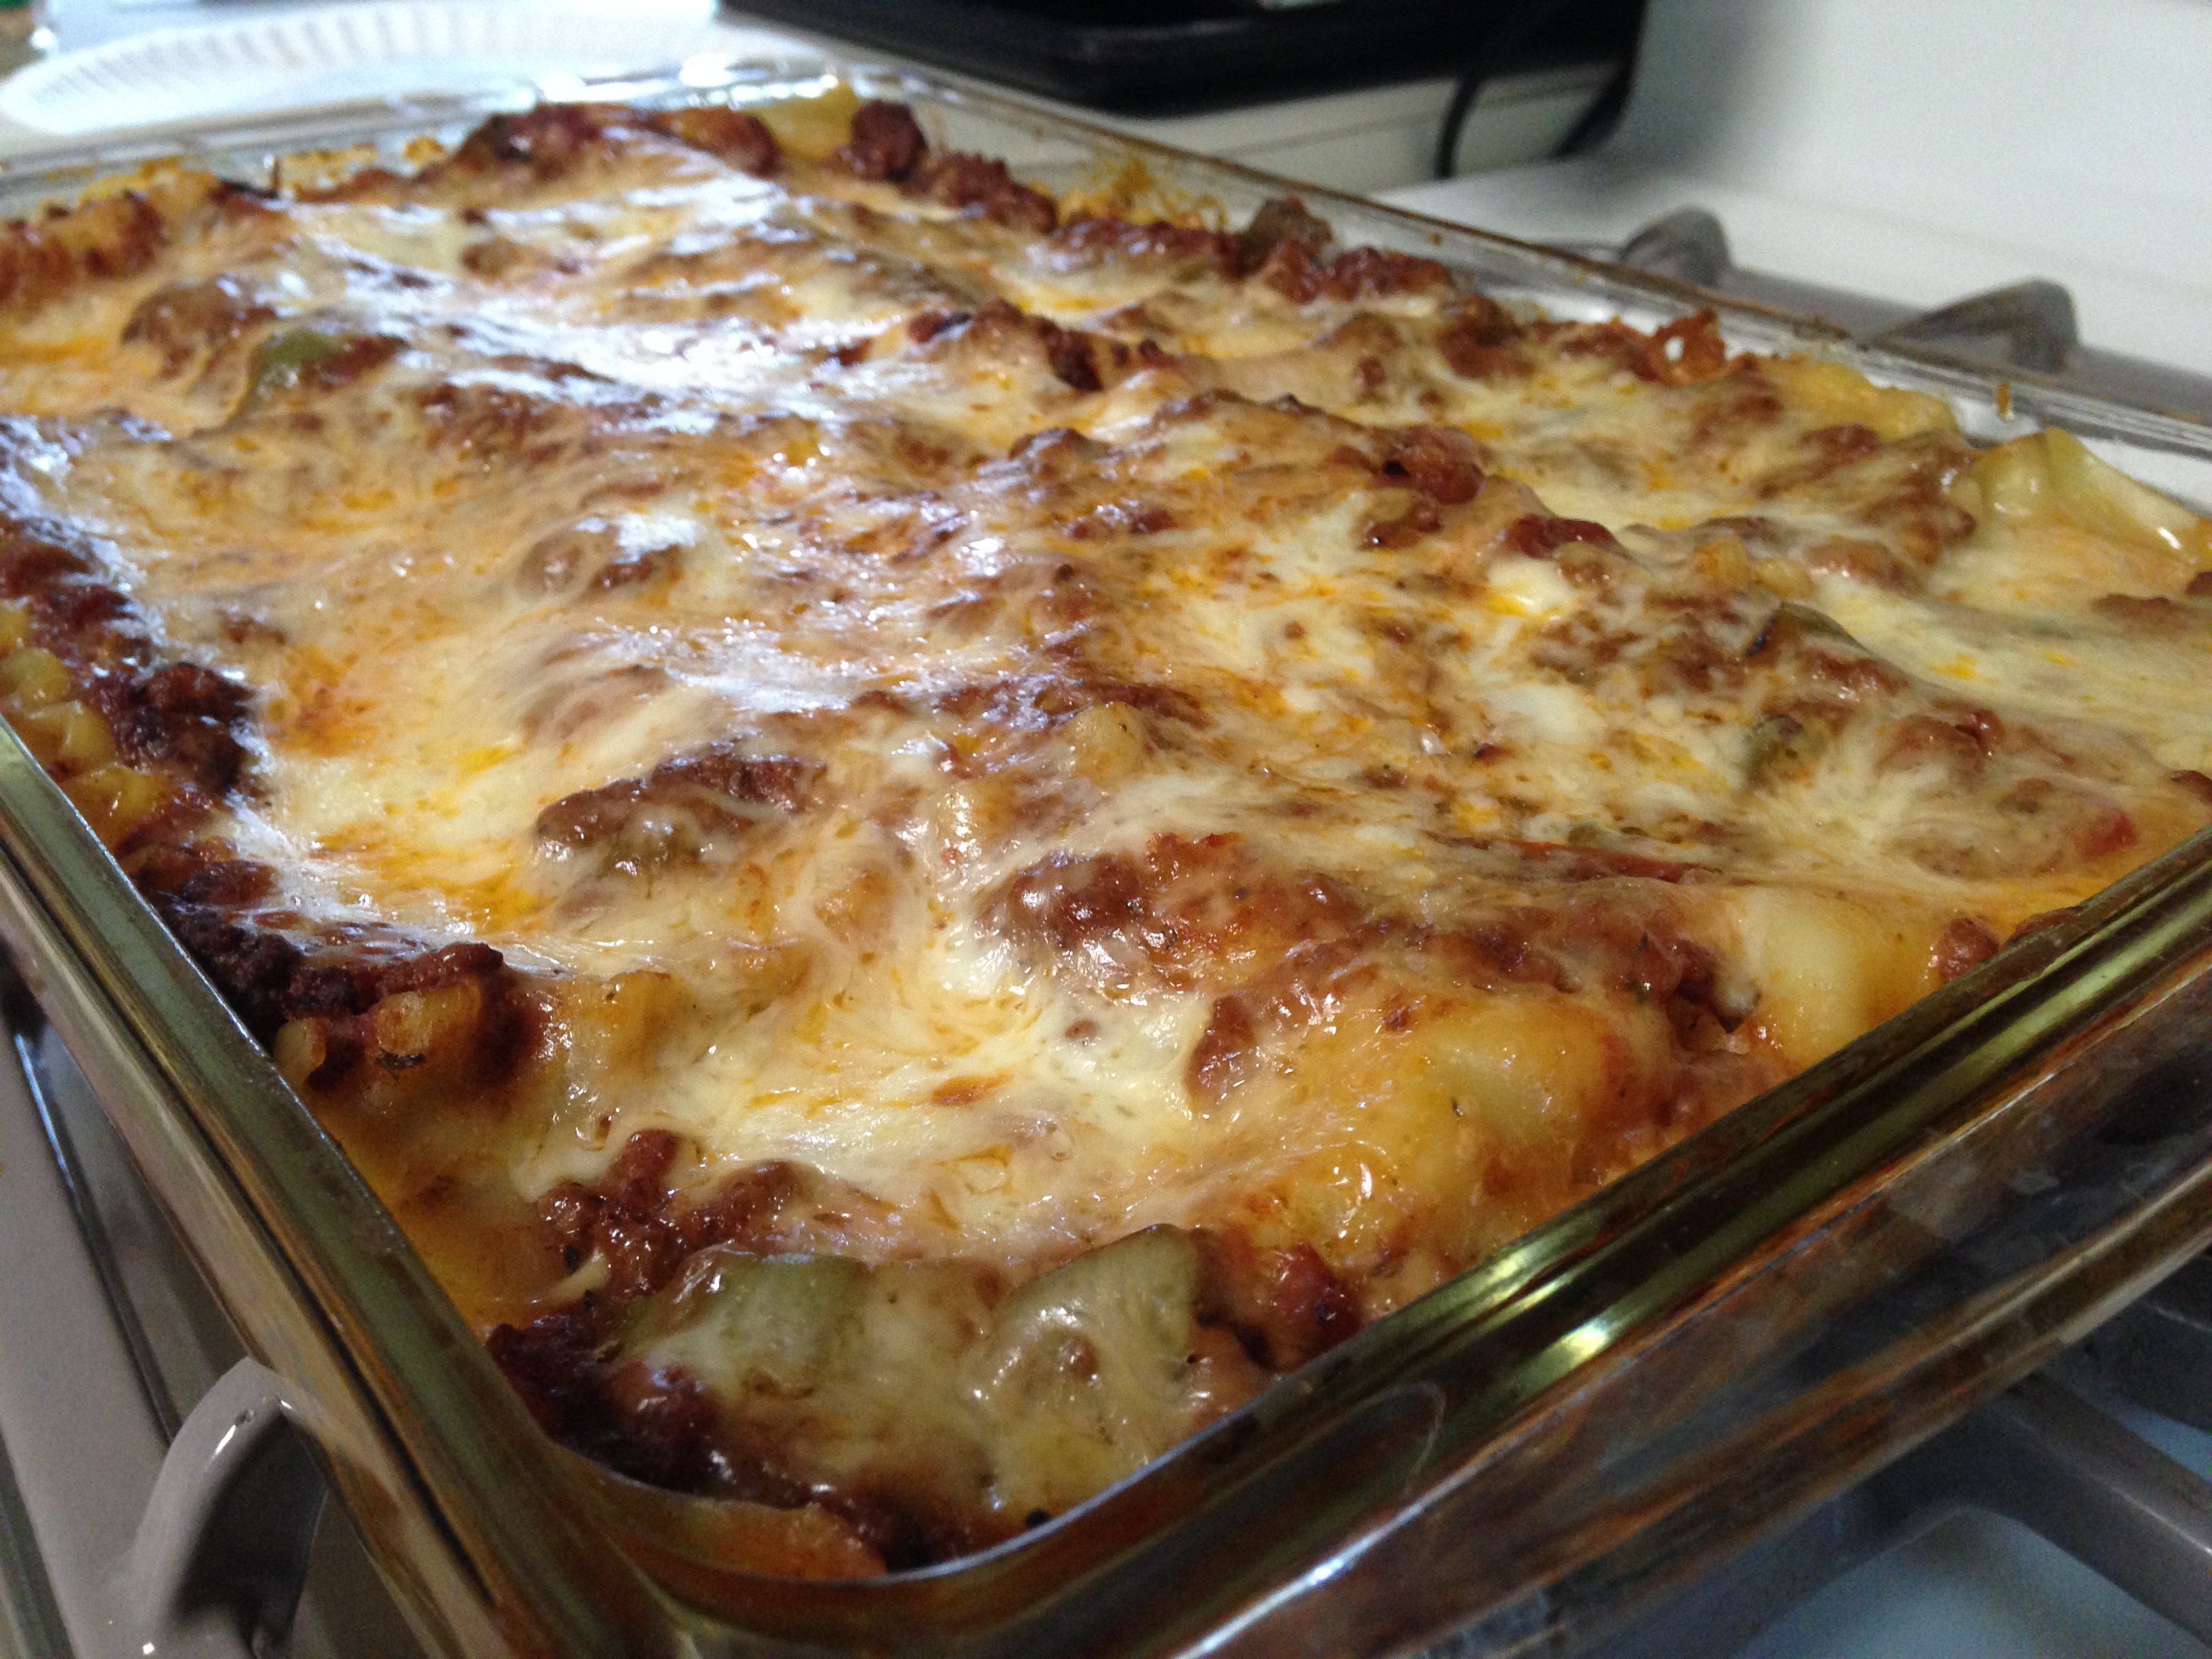
\includegraphics[height=\paperheight,%
				keepaspectratio]{./Images/Lasagna.jpg}}%
			\vfill
}}}

%VENISONBBQ
\newcommand\VenisonBBQ{%
	\put(0,0){%
		\parbox[b][\paperheight]{\paperwidth}{%
			\vfill
			\centering
			{\transparent{0.3} 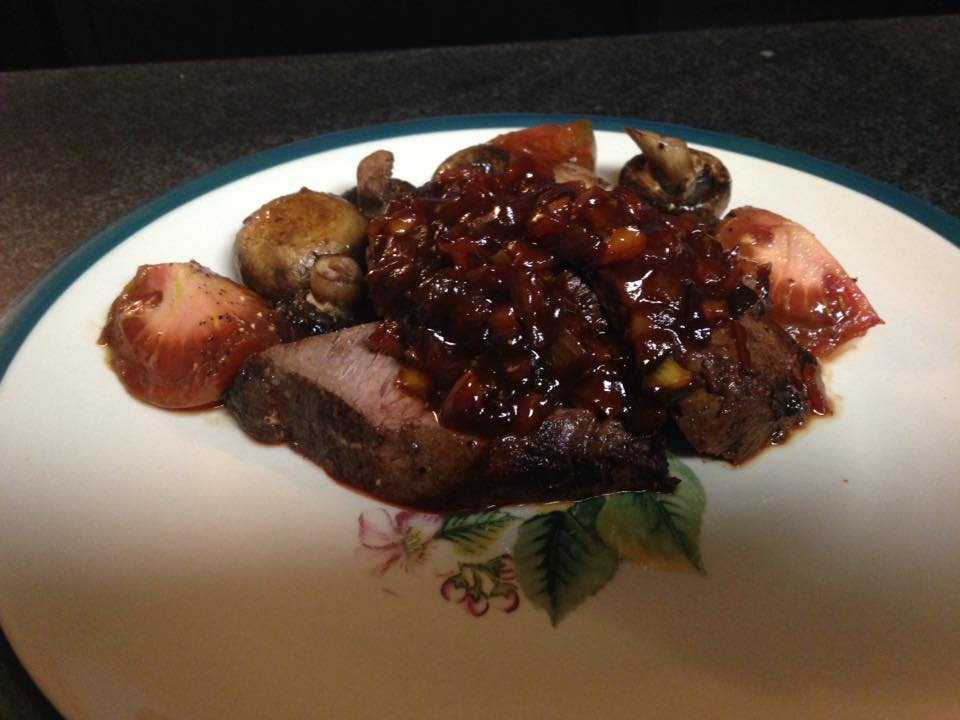
\includegraphics[height=\paperheight,%
				keepaspectratio]{./Images/VenisonBBQSauce.jpg}}%
			\vfill
}}}

%MANGOSALSA
\newcommand\MangoSalsa{%
	\put(0,0){%
		\parbox[b][\paperheight]{\paperwidth}{%
			\vfill
			\centering
			{\transparent{0.3} 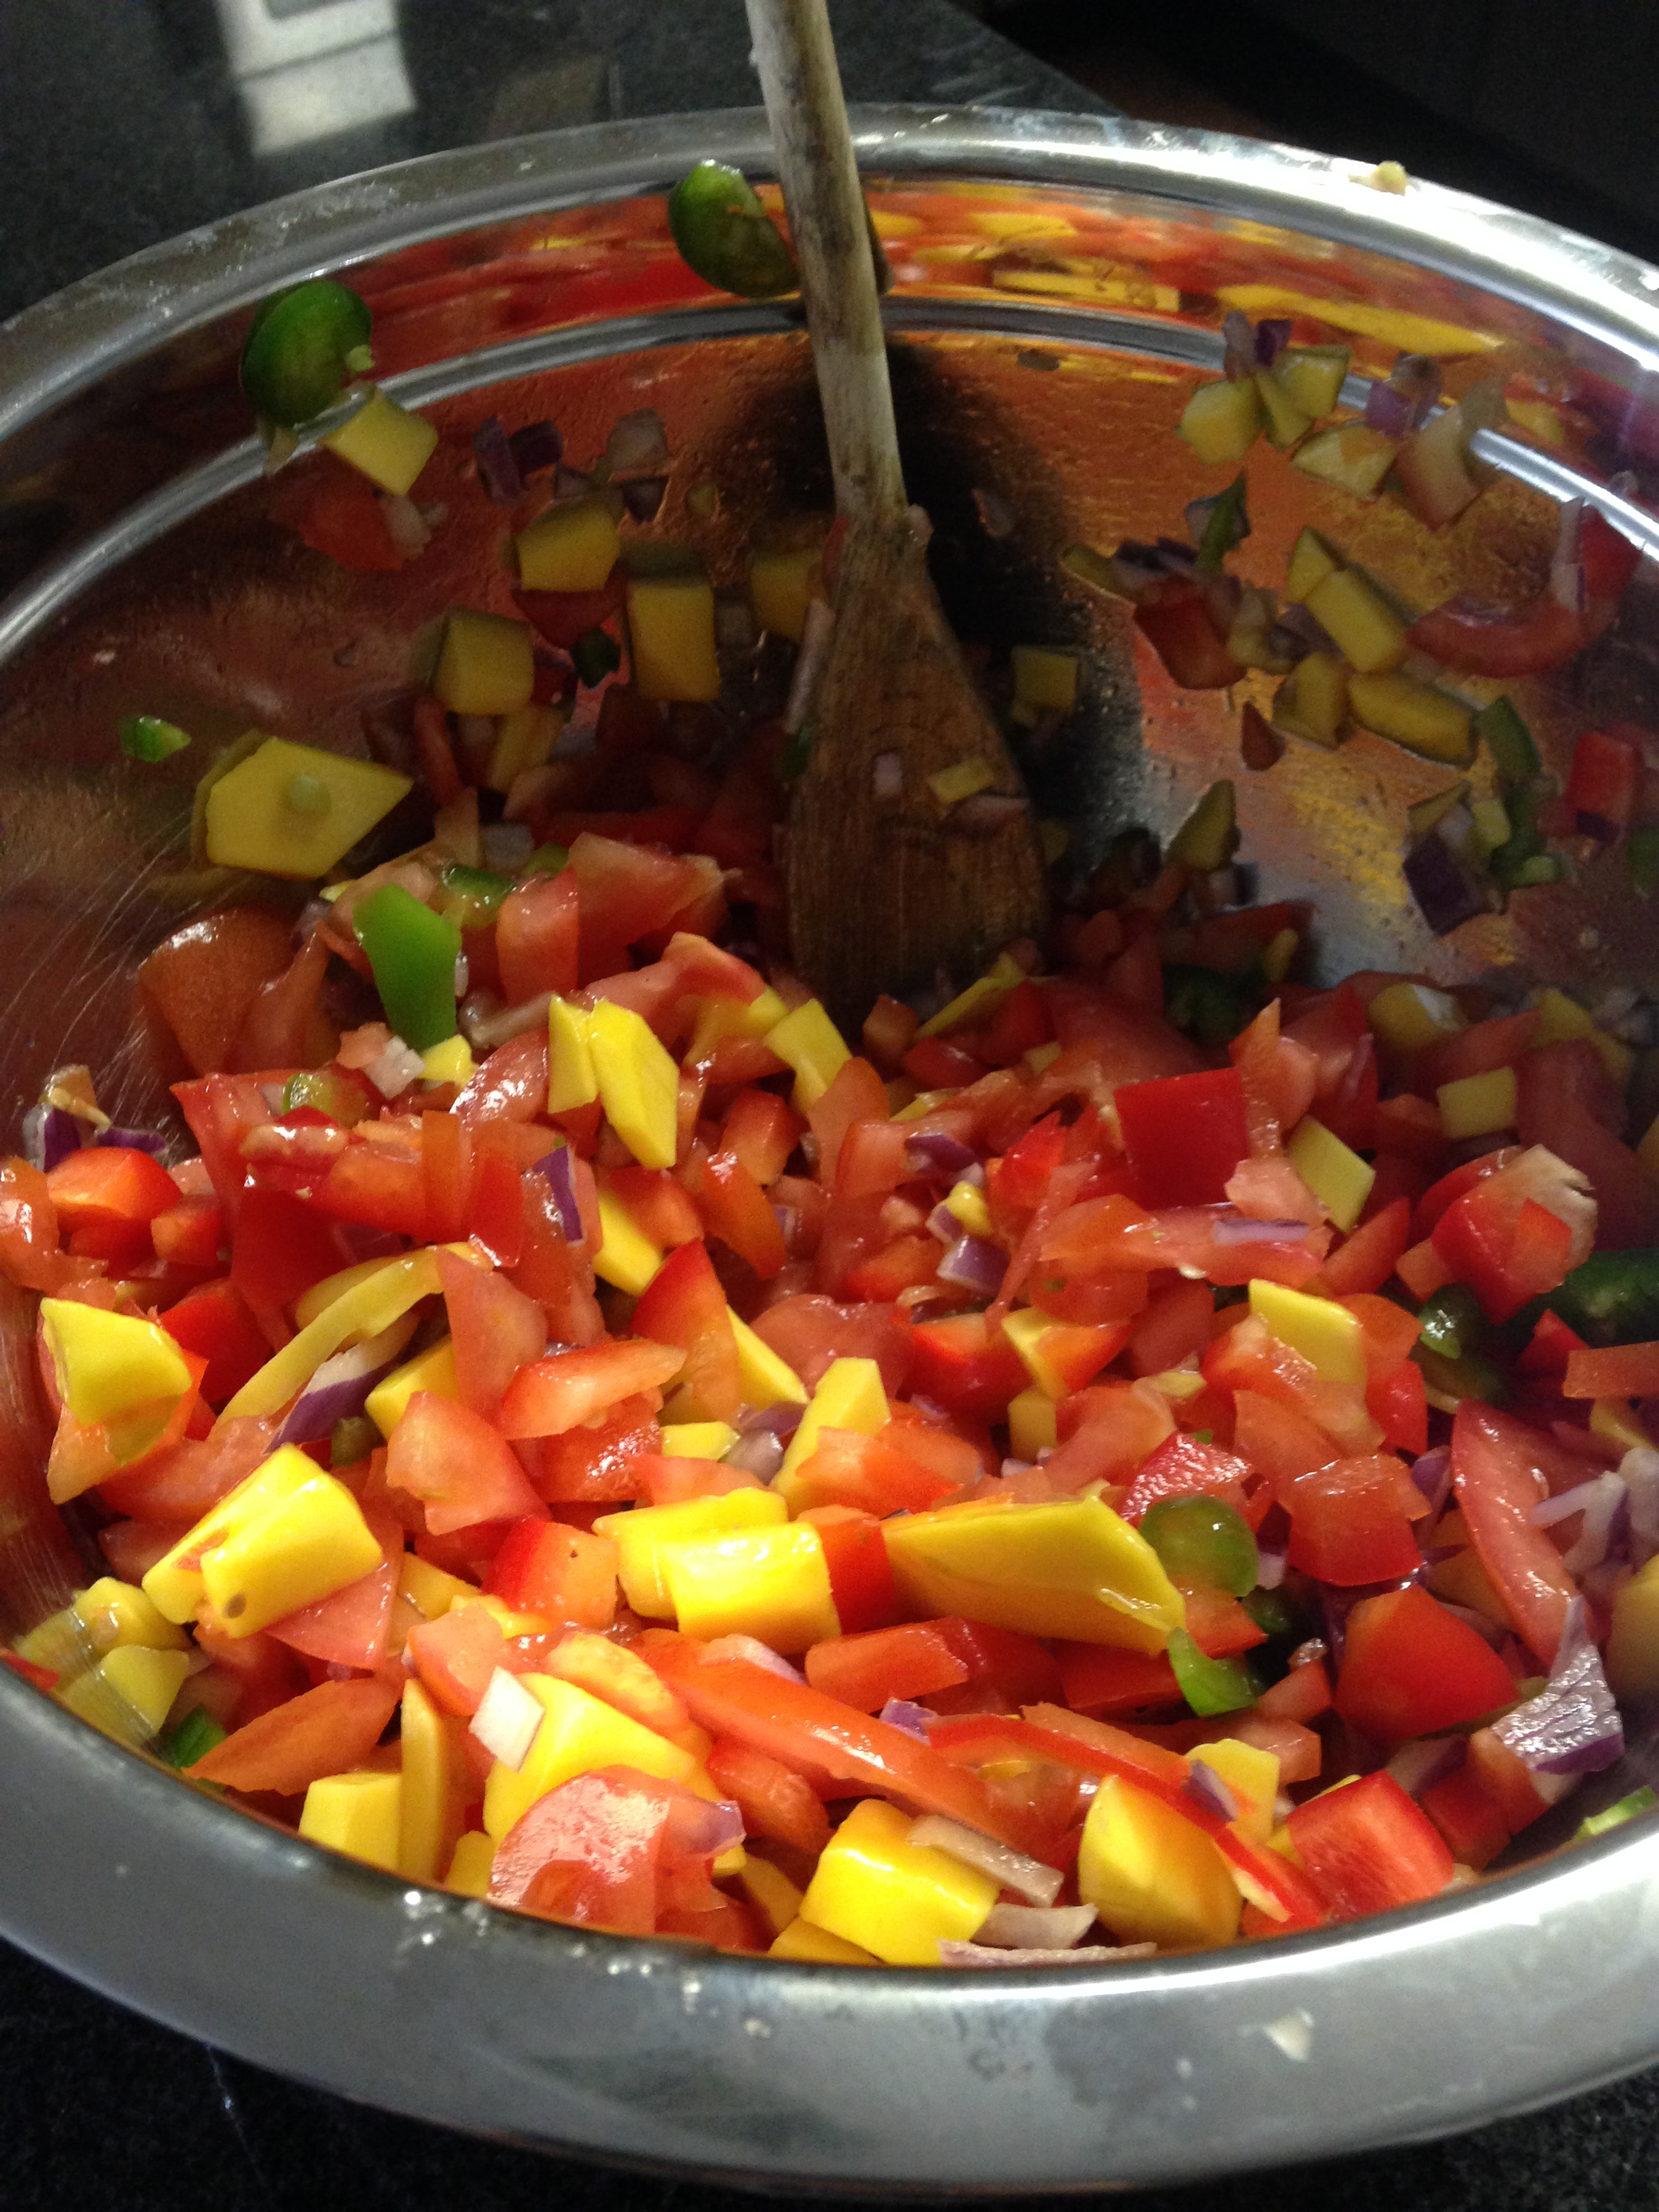
\includegraphics[height=\paperheight,%
				keepaspectratio]{./Images/MangoSalsa.jpg}}%
			\vfill
}}}

%FRUITMEDLEY
\newcommand\FruitMedley{%
	\put(0,0){%
		\parbox[b][\paperheight]{\paperwidth}{%
			\vfill
			\centering
			{\transparent{0.3} 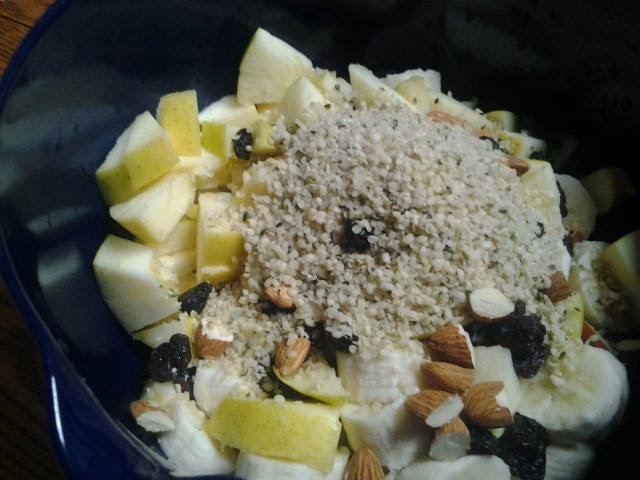
\includegraphics[height=\paperheight,%
				keepaspectratio]{./Images/FruitMedley.jpg}}%
			\vfill
}}}

%TORTILLACHIPS
\newcommand\TortillaChips{%
	\put(0,0){%
		\parbox[b][\paperheight]{\paperwidth}{%
			\vfill
			\centering
			{\transparent{0.3} 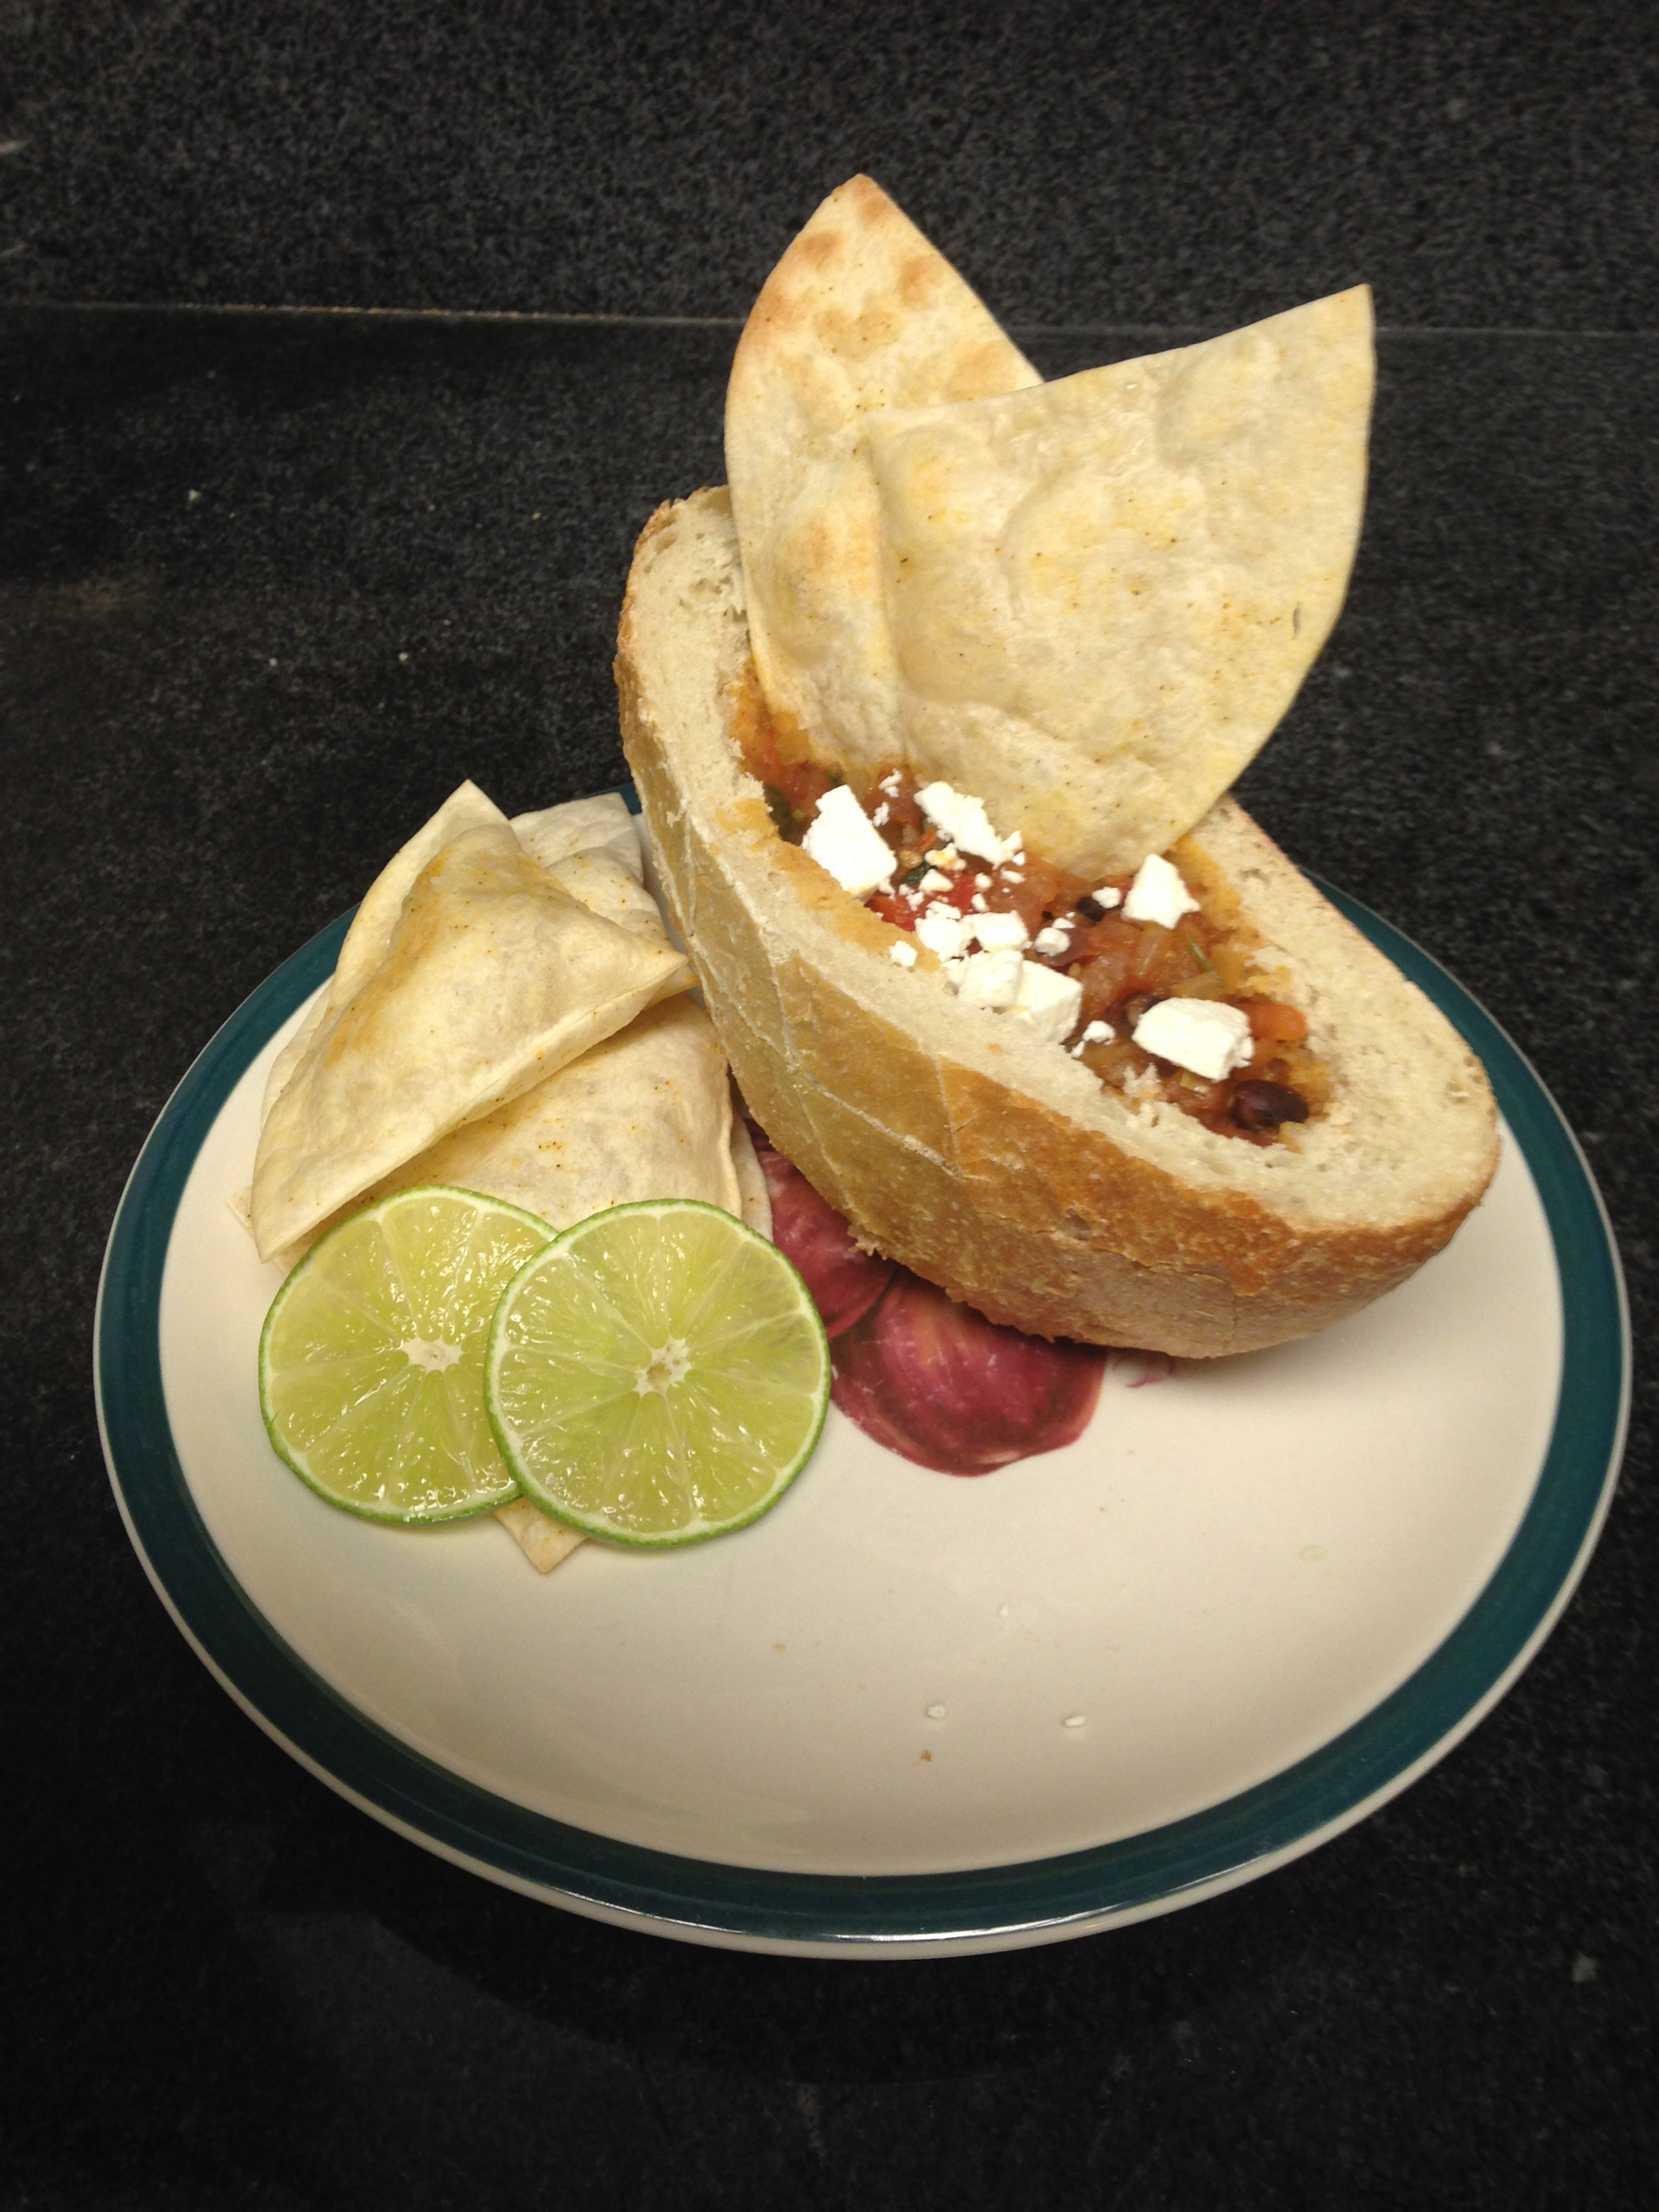
\includegraphics[height=\paperheight,%
				keepaspectratio]{./Images/TortillaChips.jpg}}%
			\vfill
}}}

%FRUITTOPPING
\newcommand\FruitTopping{%
	\put(0,0){%
		\parbox[b][\paperheight]{\paperwidth}{%
			\vfill
			\centering
			{\transparent{0.3} 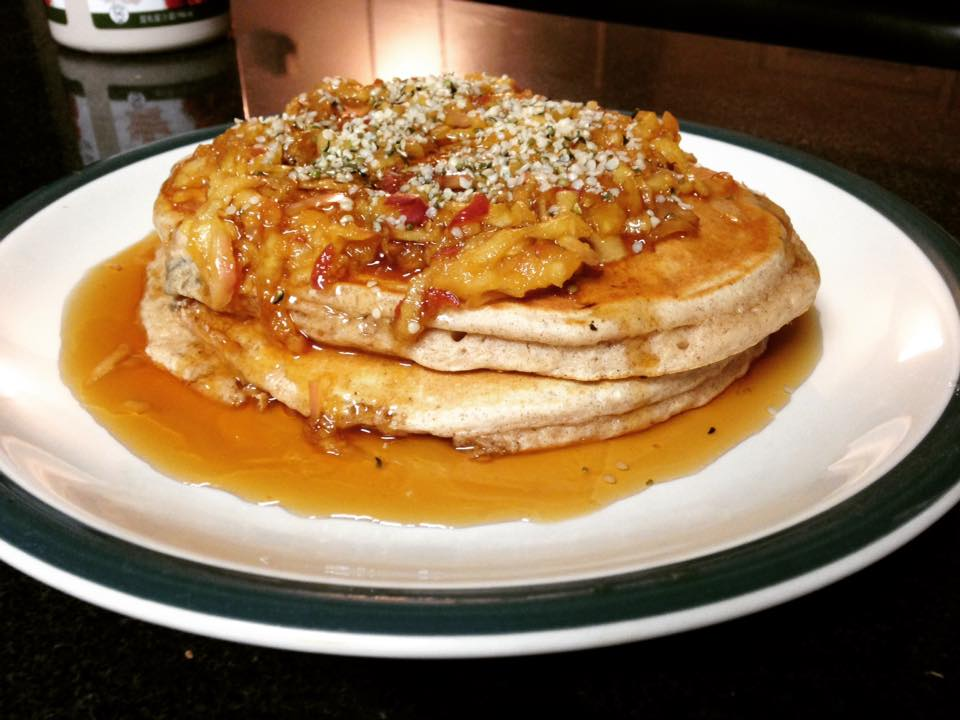
\includegraphics[height=\paperheight,%
				keepaspectratio]{./Images/PancakesWithApple.jpg}}%
			\vfill
}}}

%LEMONPOPPYSEED
\newcommand\LemonPoppyseed{%
	\put(0,0){%
		\parbox[b][\paperheight]{\paperwidth}{%
			\vfill
			\centering
			{\transparent{0.3} 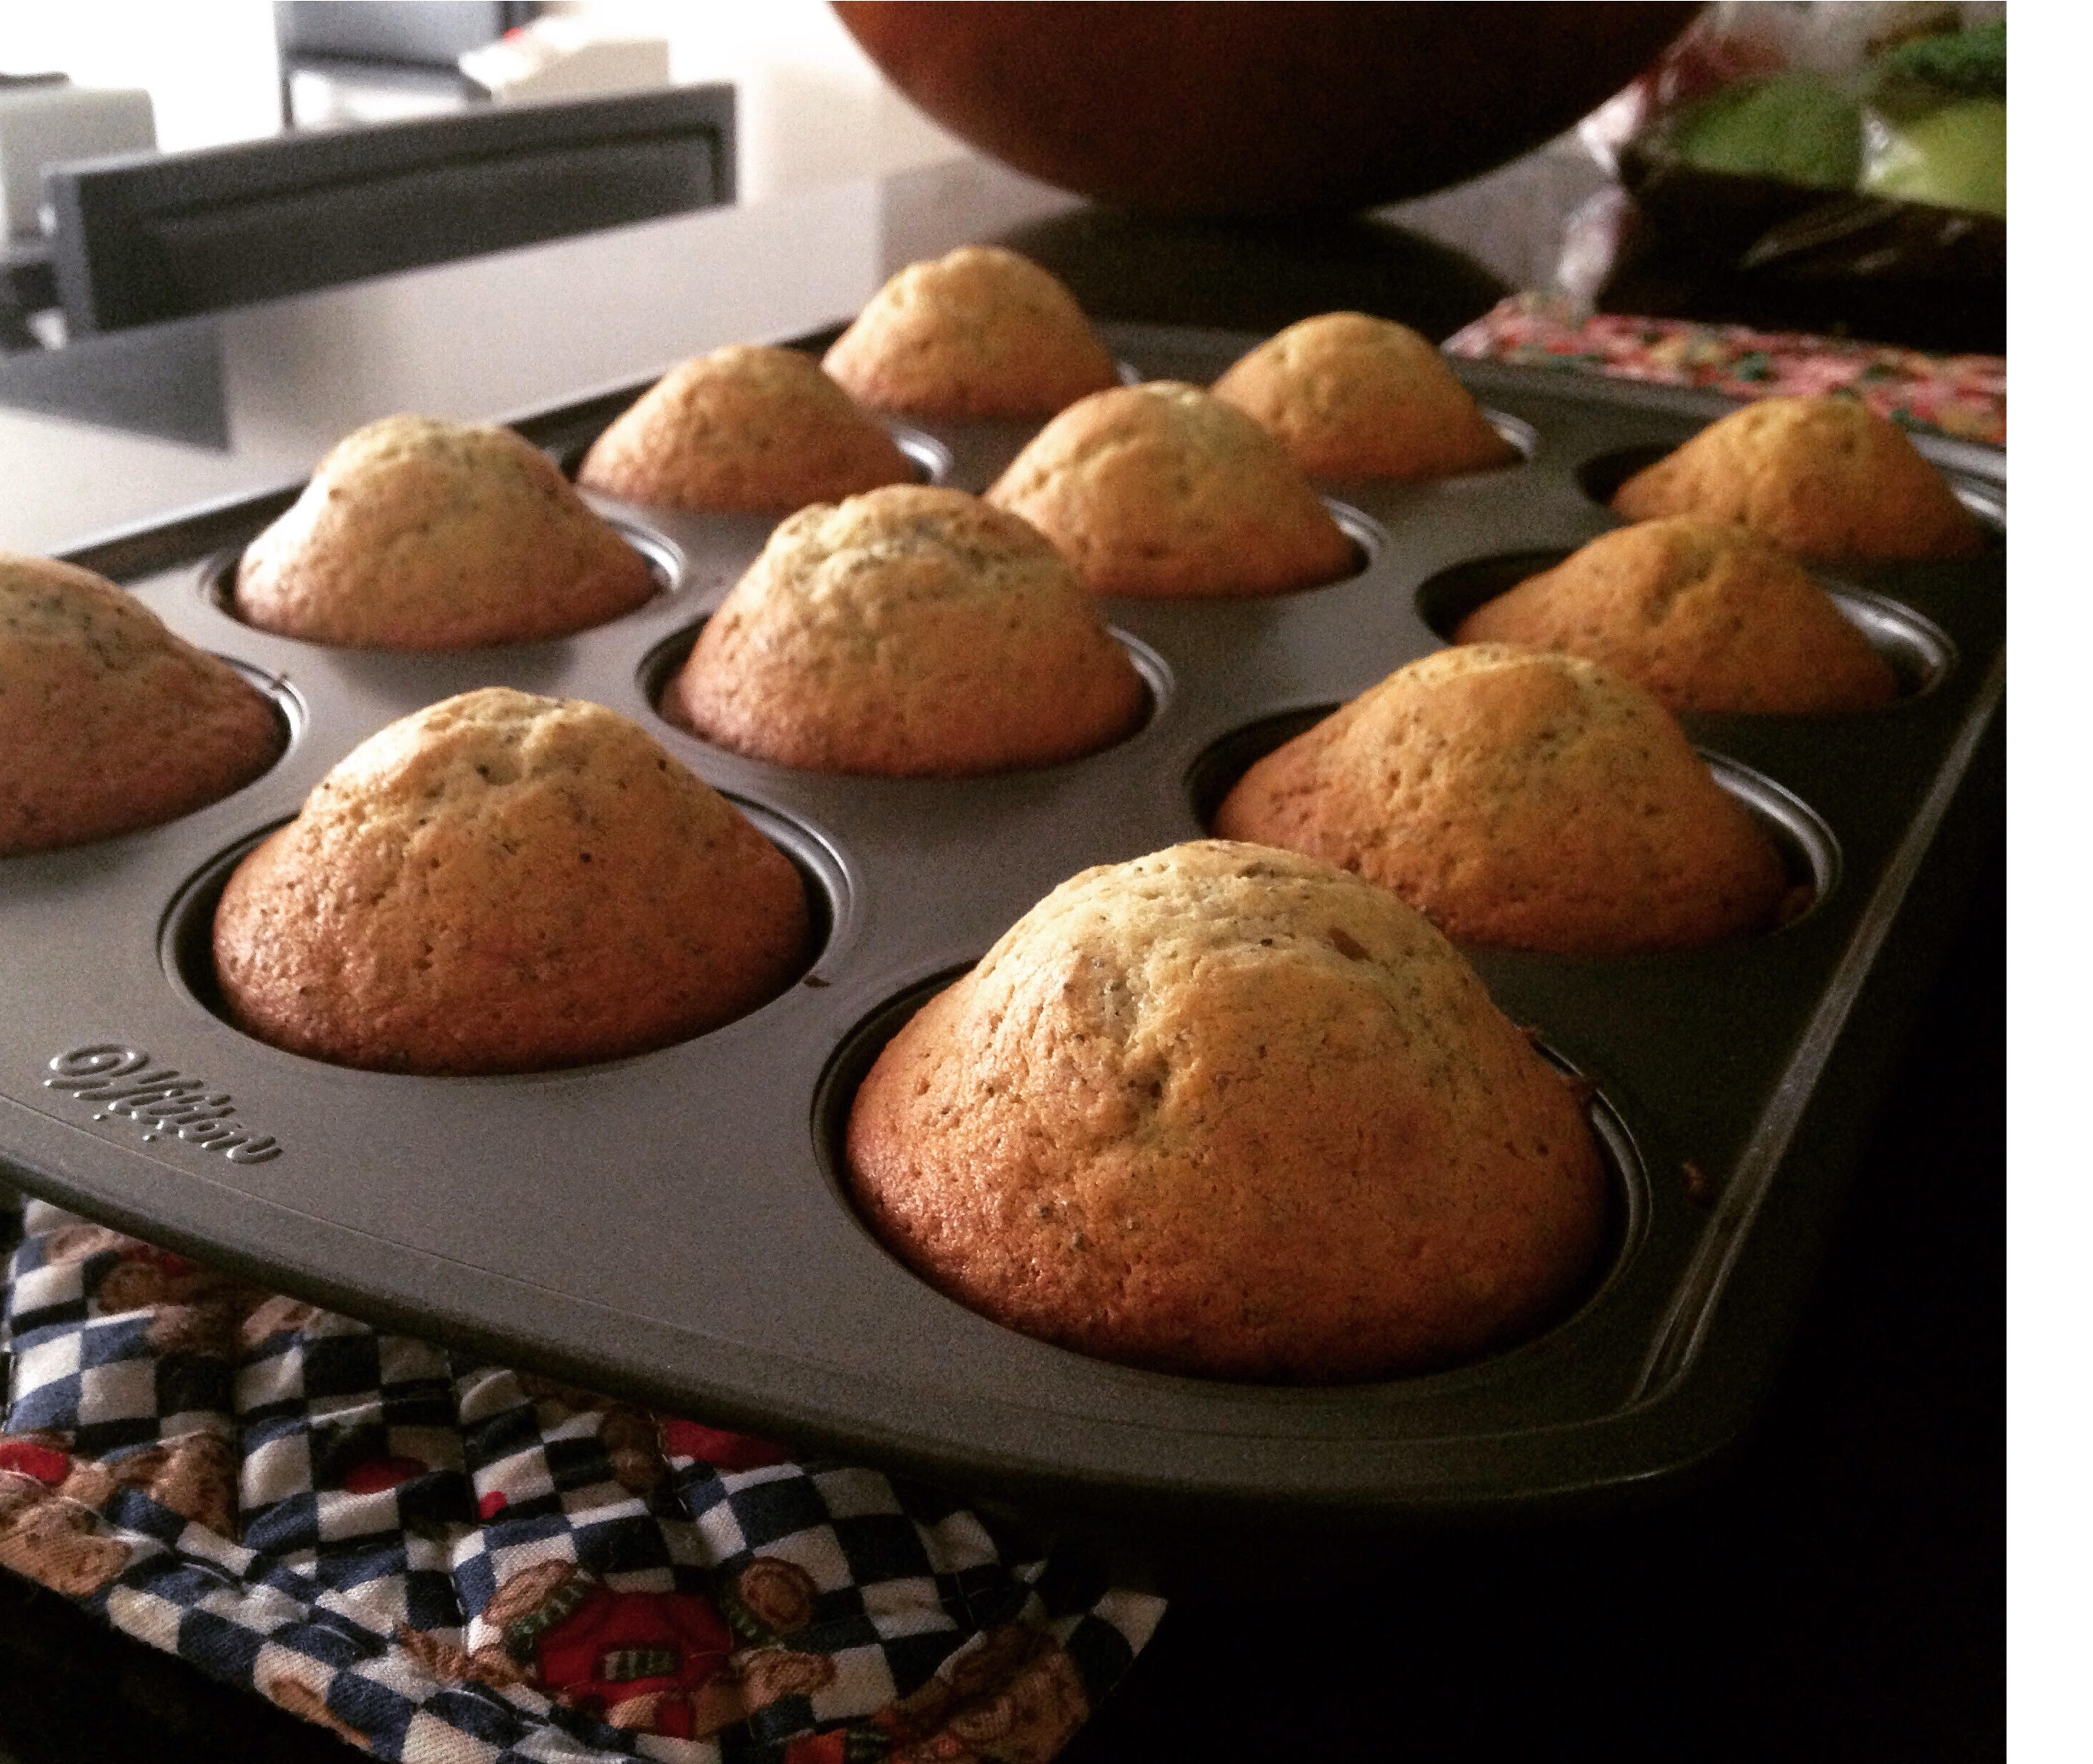
\includegraphics[height=\paperheight,%
				keepaspectratio]{./Images/LemonPoppyseed.jpg}}%
			\vfill
}}}

%TOWERGARDEN
\newcommand\TowerGarden{%
	\put(0,0){%
		\parbox[b][\paperheight]{\paperwidth}{%
			\vfill
			\centering
			{\transparent{0.3} 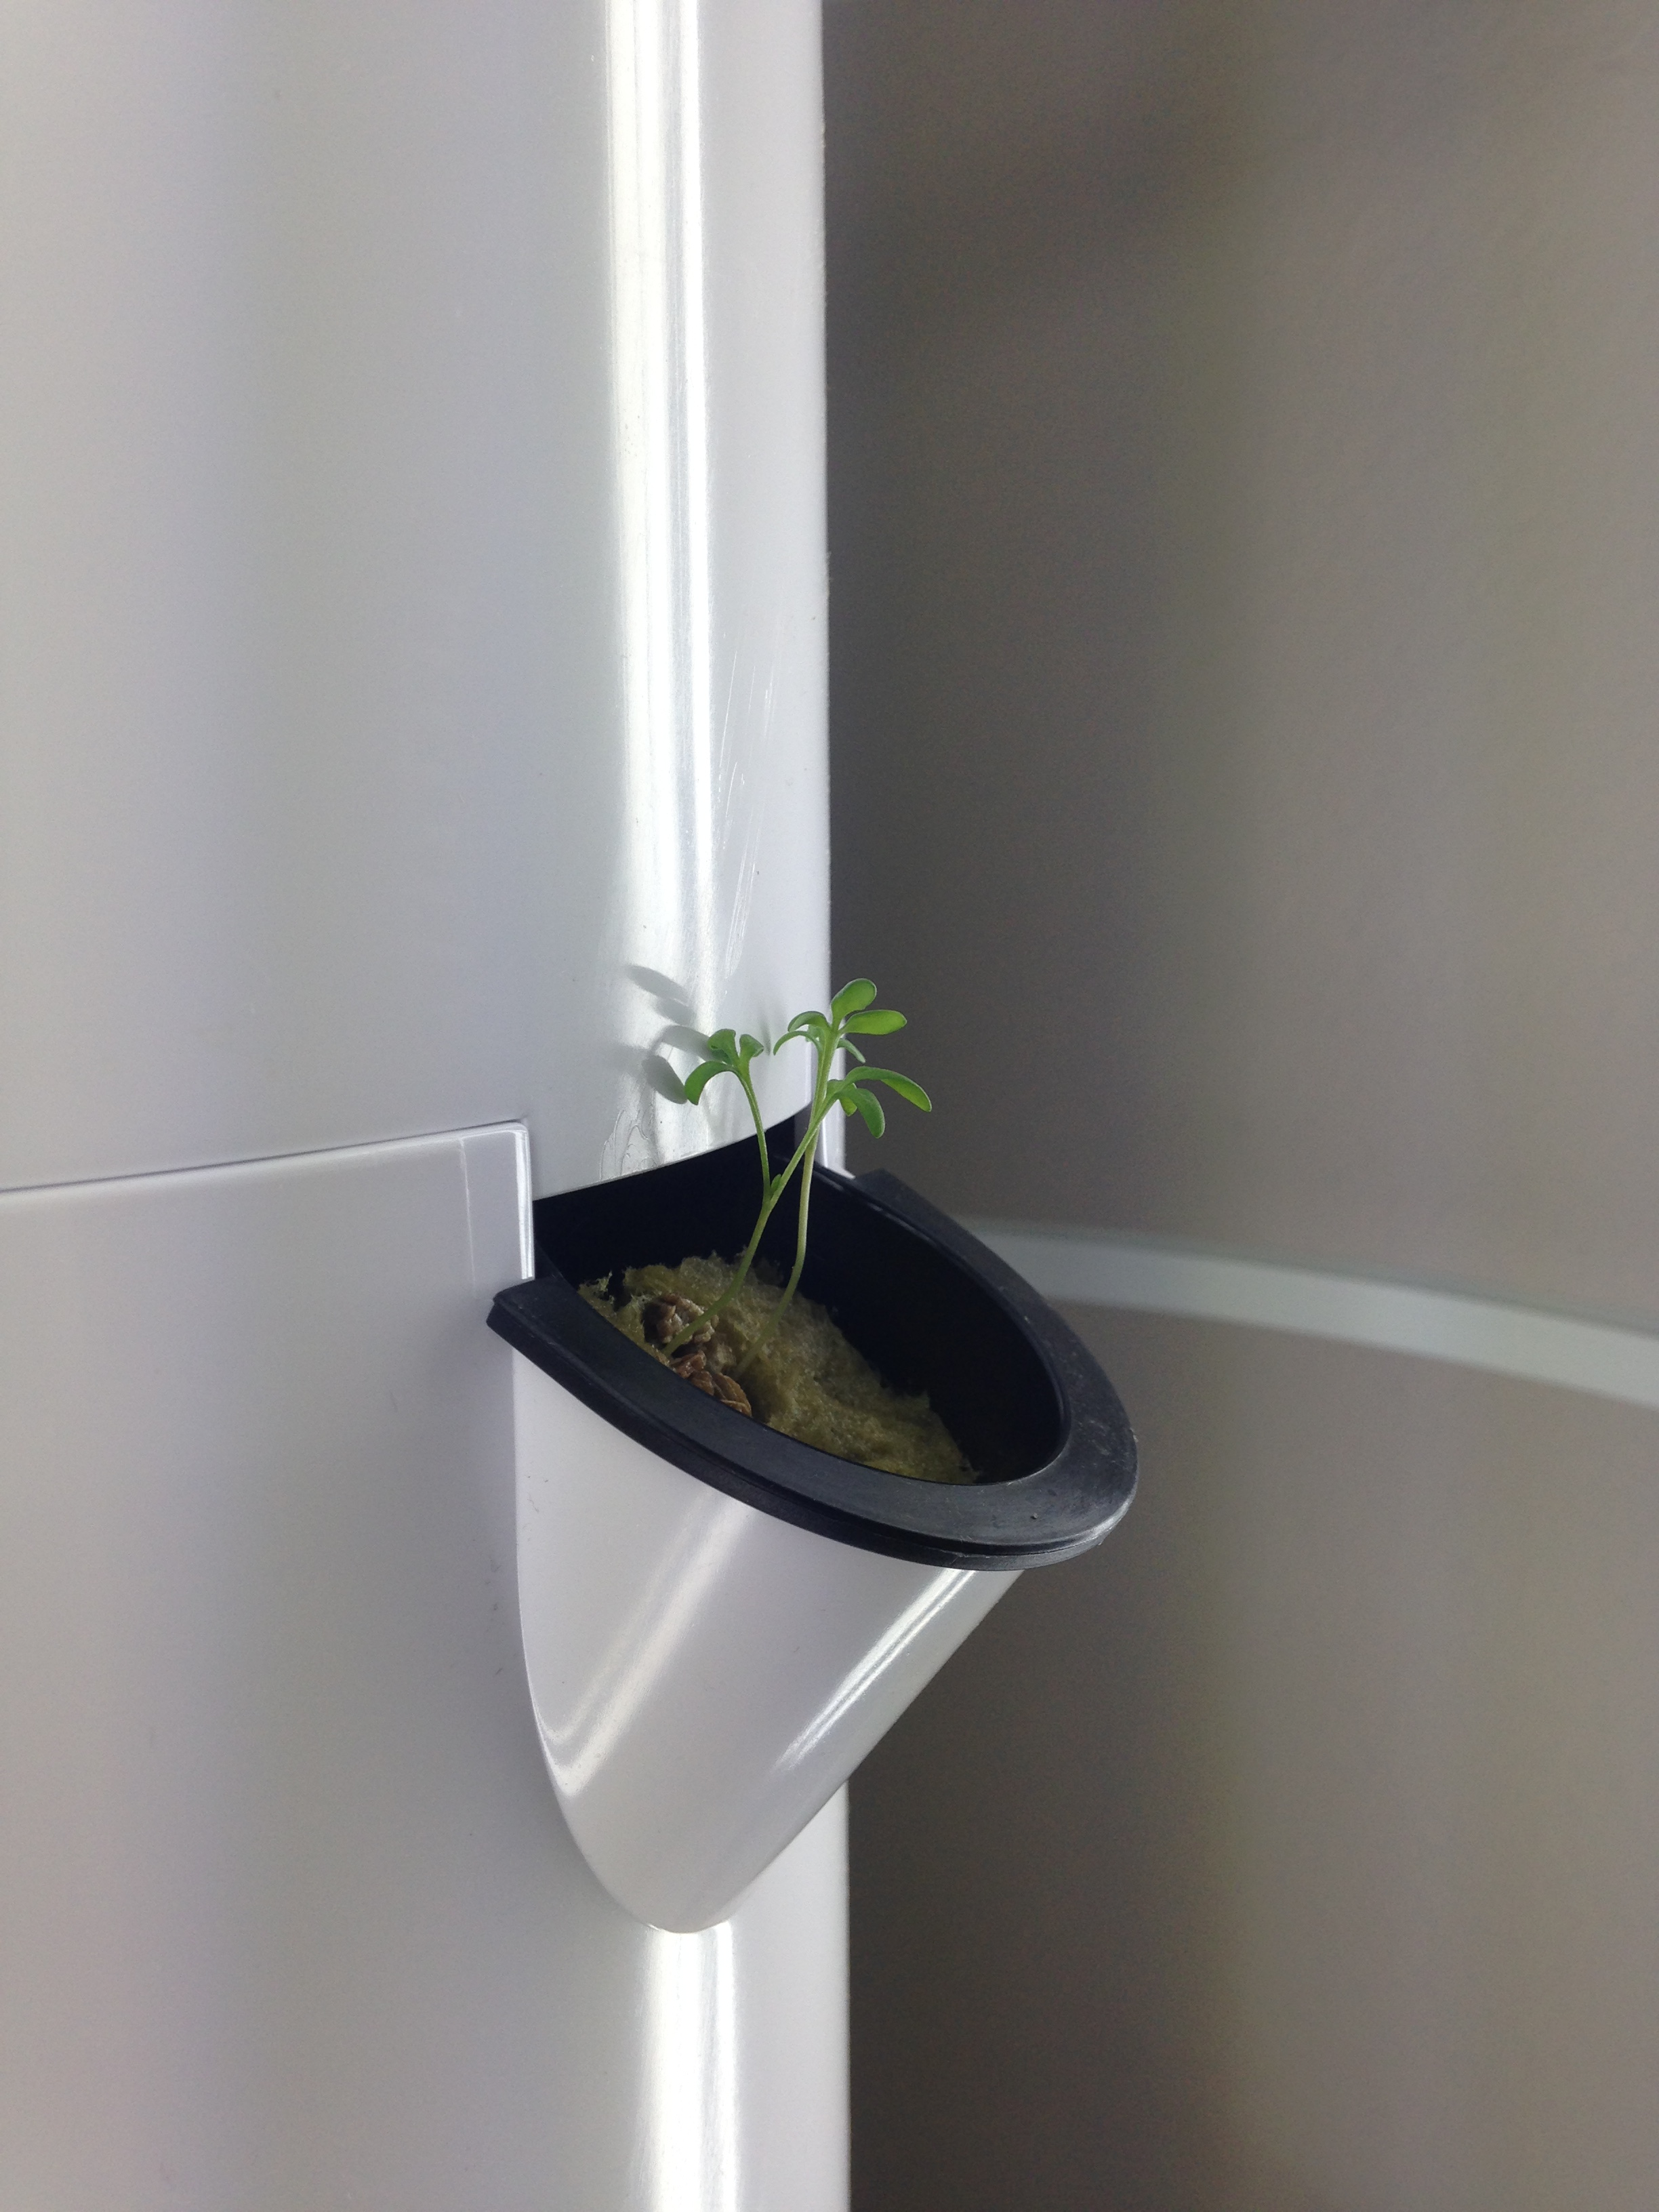
\includegraphics[height=\paperheight,%
				keepaspectratio]{./Images/TowerGarden.jpg}}%
			\vfill
}}}

%SAFFRONICECREAM
\newcommand\SaffronIceCream{%
	\put(0,0){%
		\parbox[b][\paperheight]{\paperwidth}{%
			\vfill
			\centering
			{\transparent{0.3} 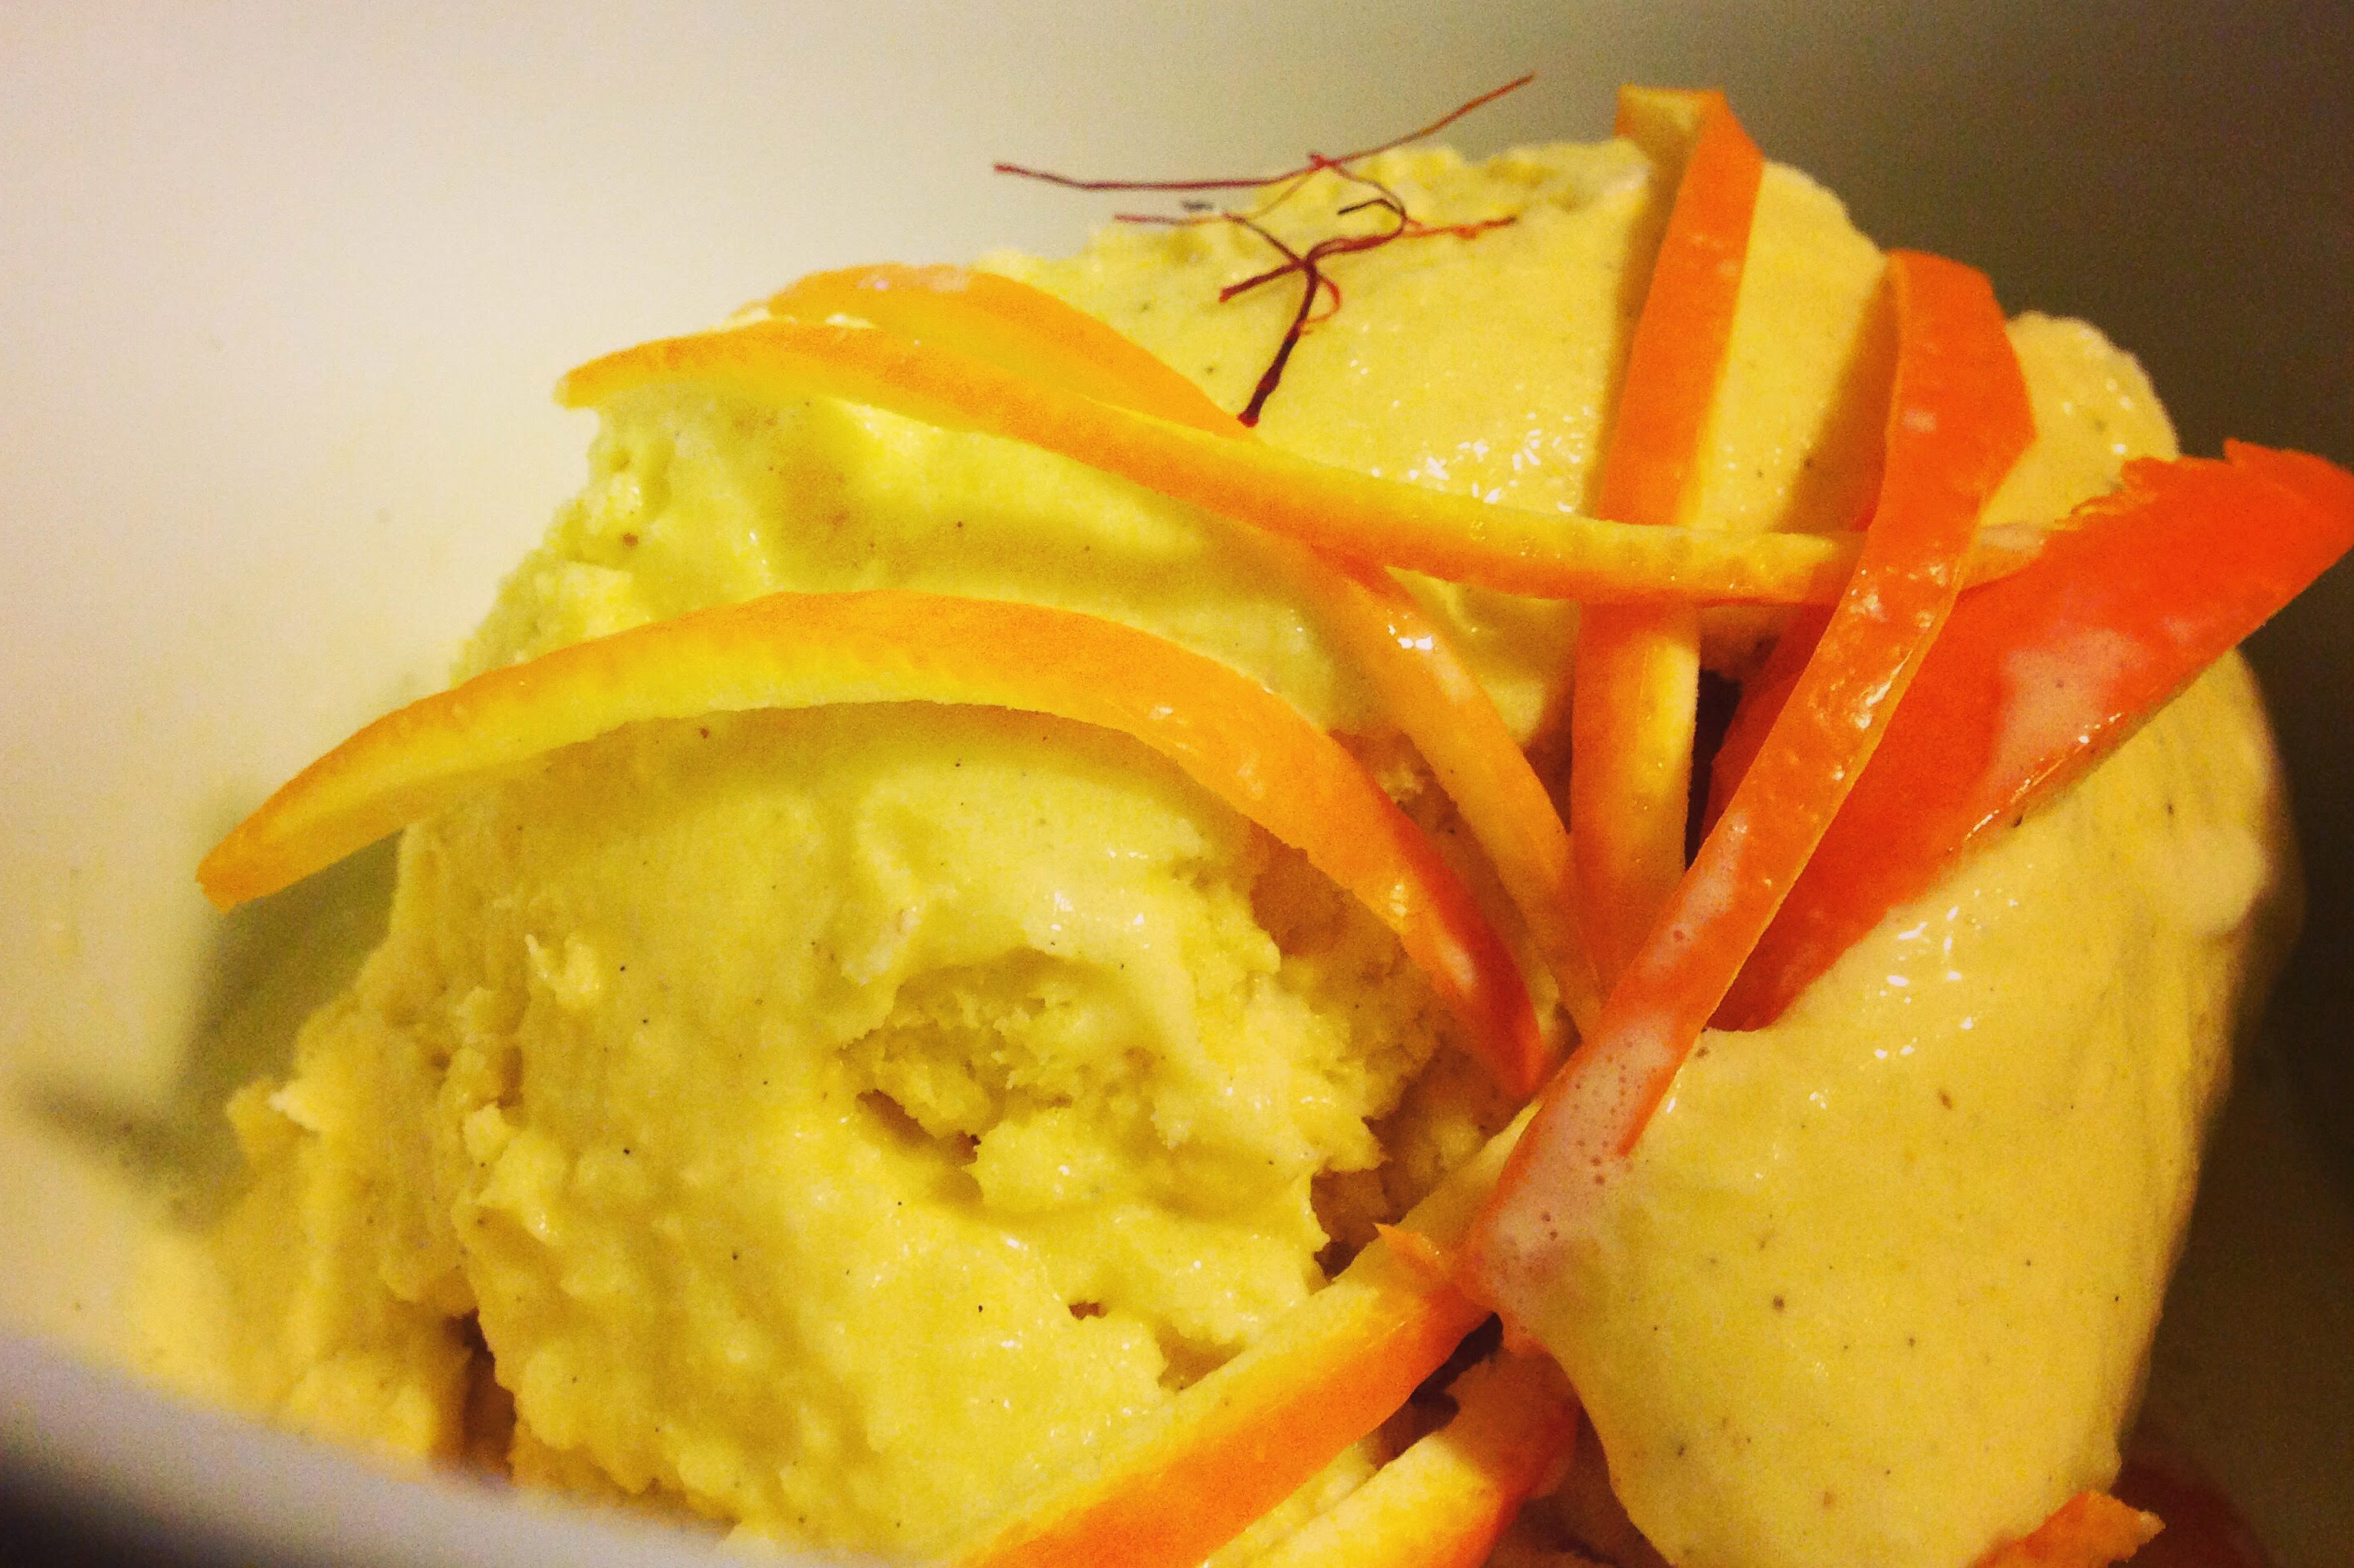
\includegraphics[height=\paperheight,%
				keepaspectratio]{./Images/SaffronIceCream.jpg}}%
			\vfill
}}}

%STRAWBERRYSALAD
\newcommand\StrawberrySalad{%


	\put(0,0){%
		\parbox[b][\paperheight]{\paperwidth}{%
			\vfill
			\centering
			{\transparent{0.3} 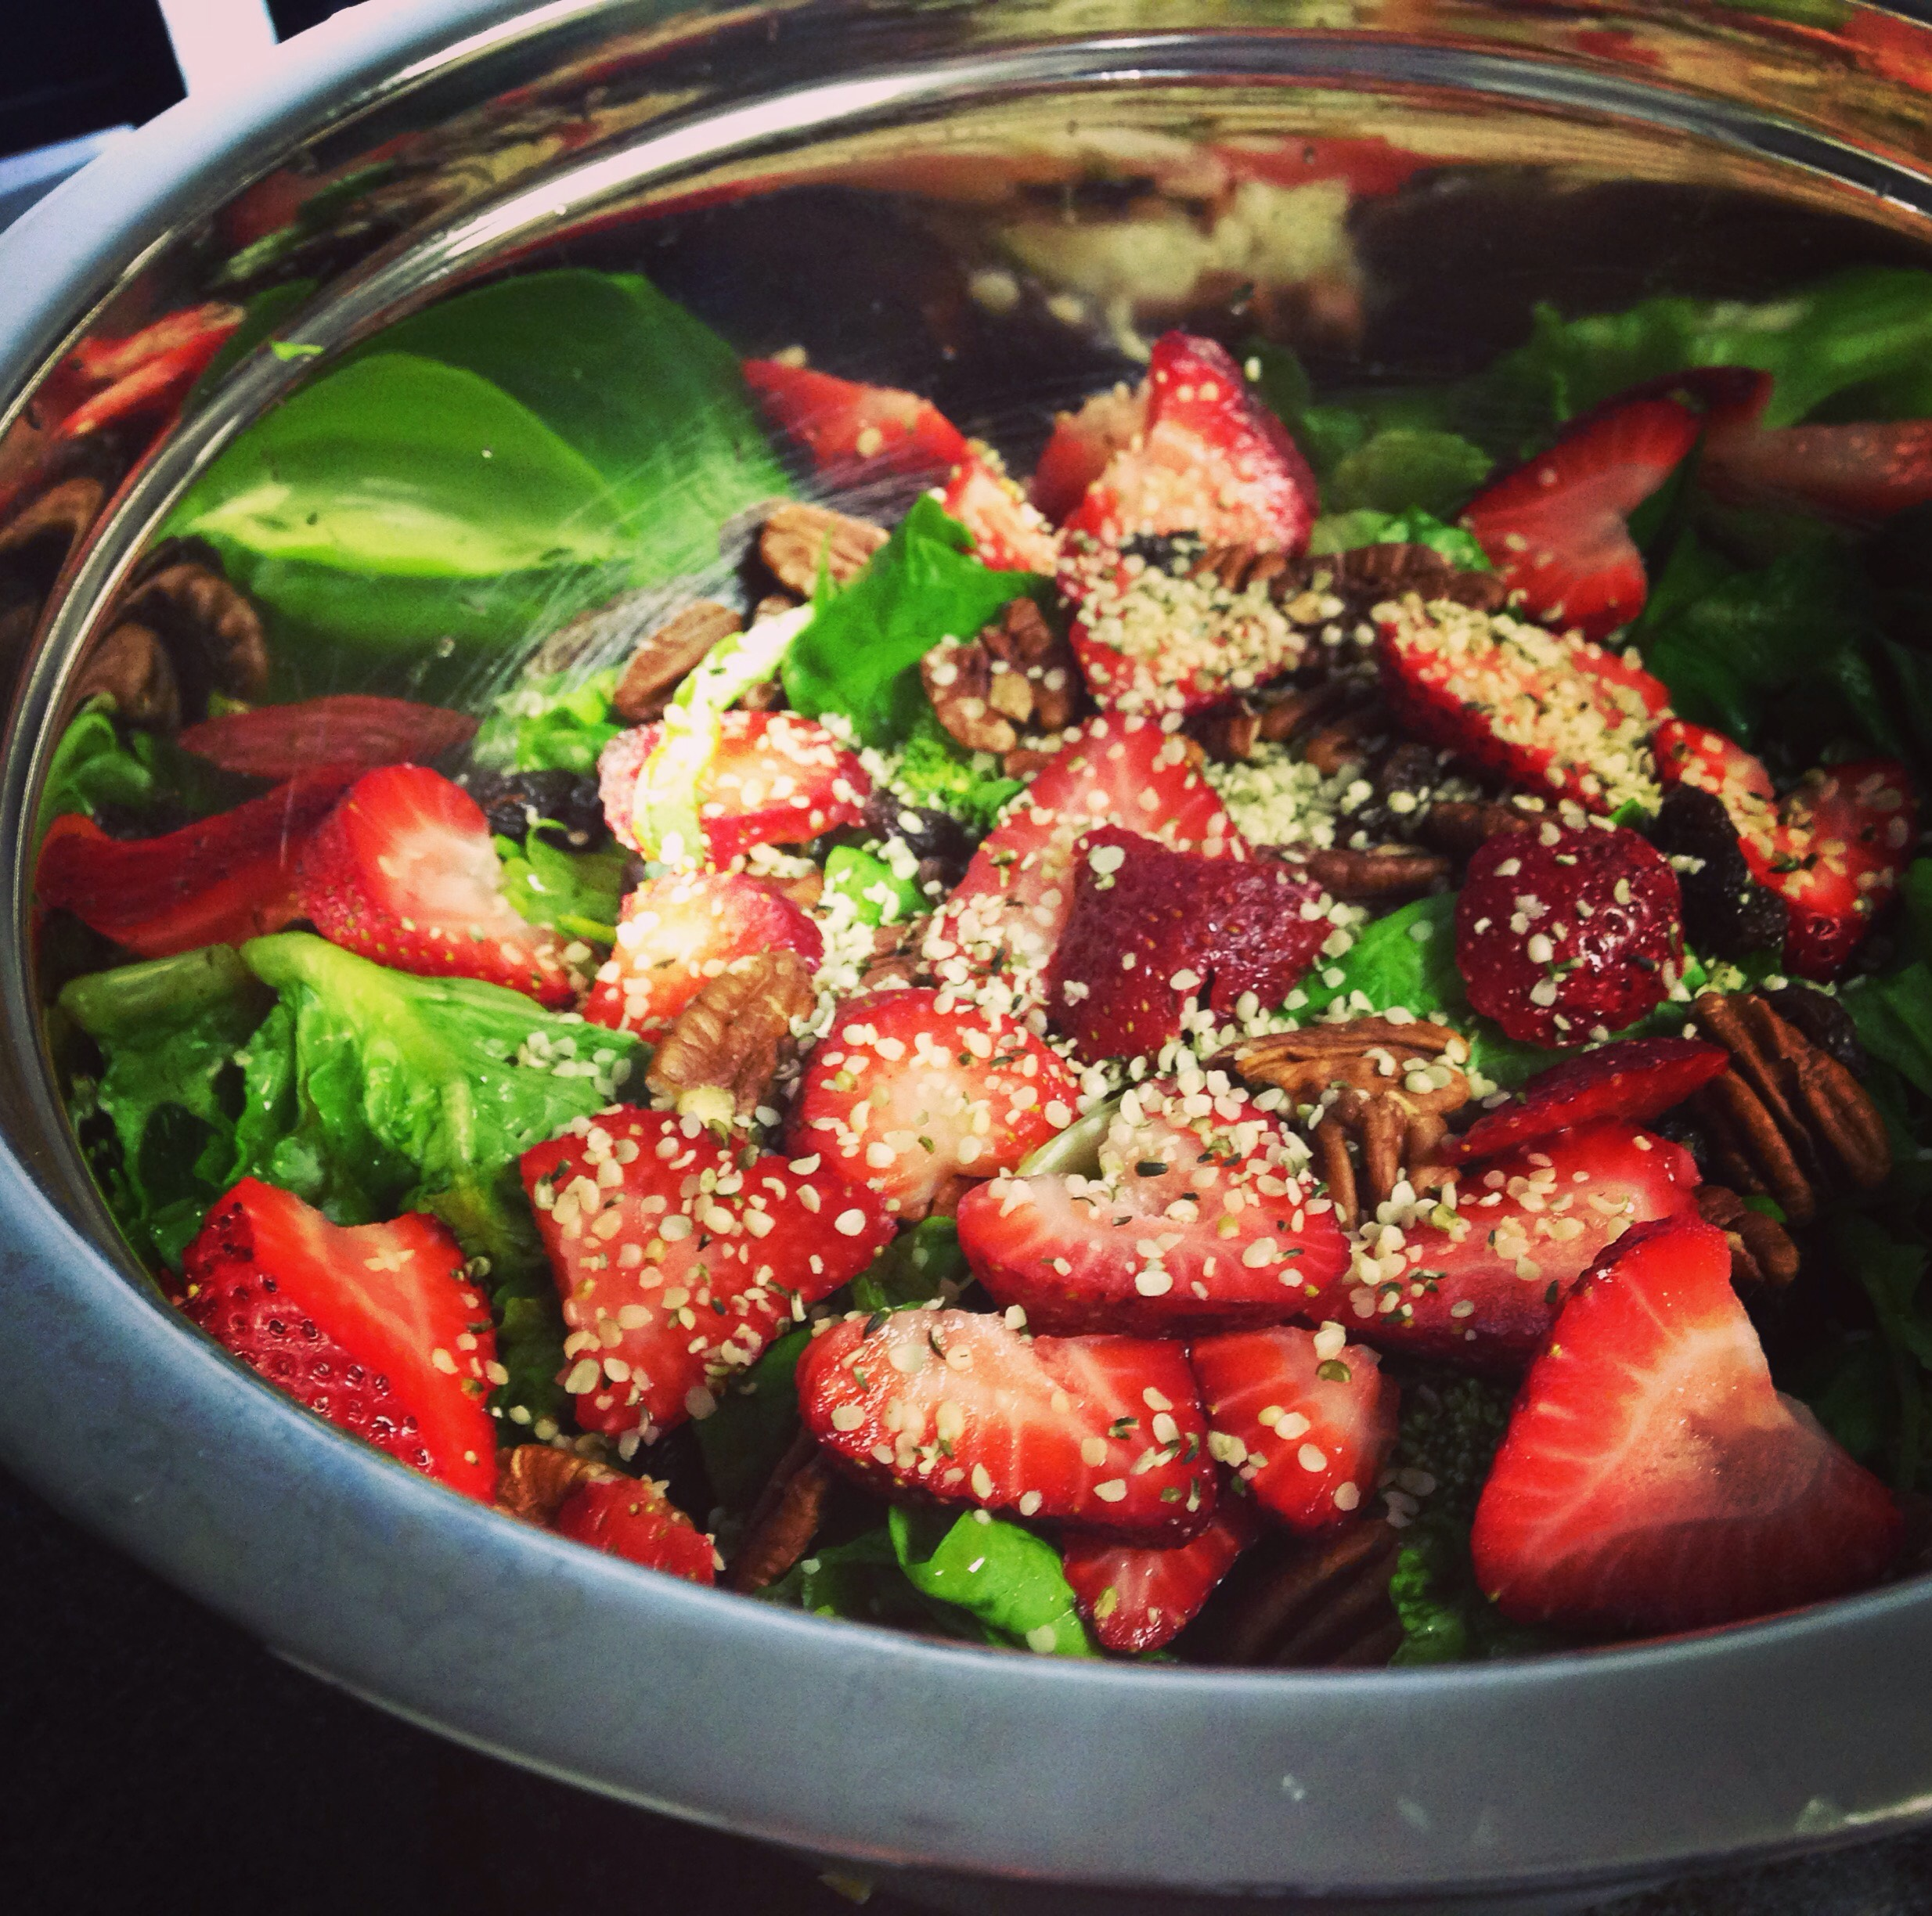
\includegraphics[height=\paperheight,%
				keepaspectratio]{./Images/StrawberrySalad.jpg}}%
			\vfill
}}}

%SALMONSALAD
\newcommand\SalmonSalad{%
	
	
	\put(0,0){%
		\parbox[b][\paperheight]{\paperwidth}{%
			\vfill
			\centering
			{\transparent{0.3} 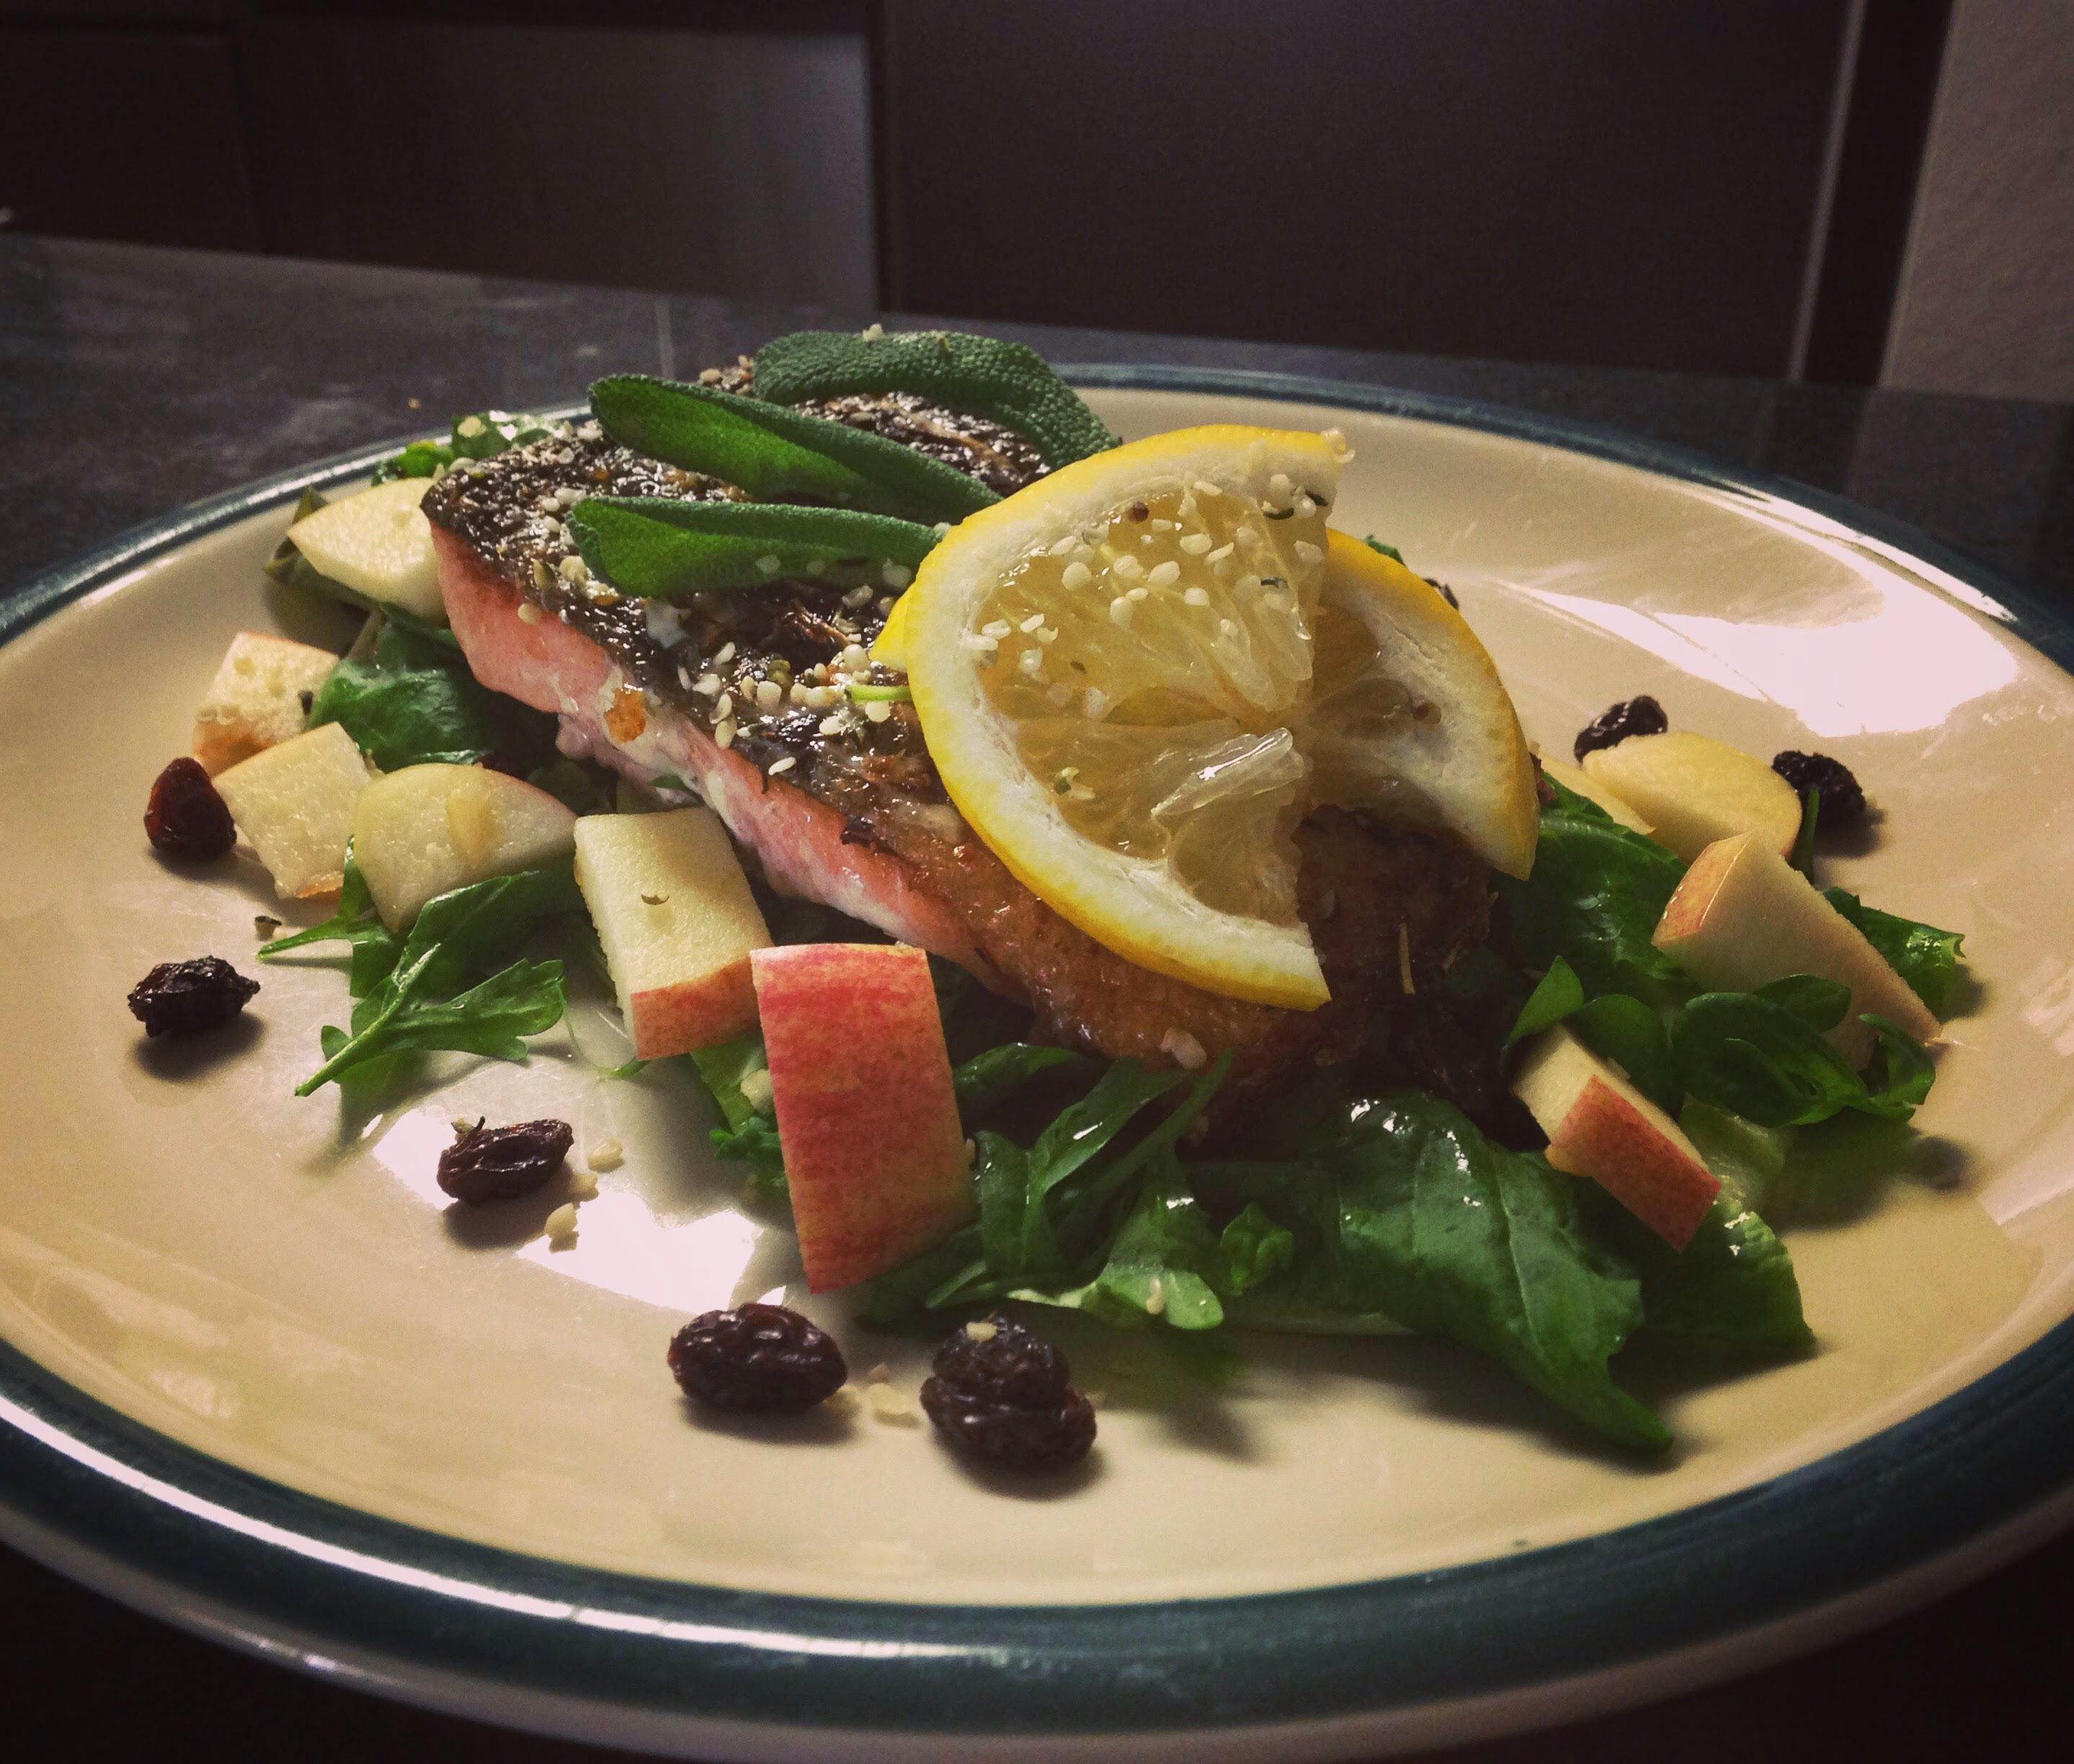
\includegraphics[height=\paperheight,%
				keepaspectratio]{./Images/SalmonSalad.jpg}}%
			\vfill
}}}

%SALMONSALAD
\newcommand\QuinoaPatties{%
	
	
	\put(0,0){%
		\parbox[b][\paperheight]{\paperwidth}{%
			\vfill
			\centering
			{\transparent{0.3} 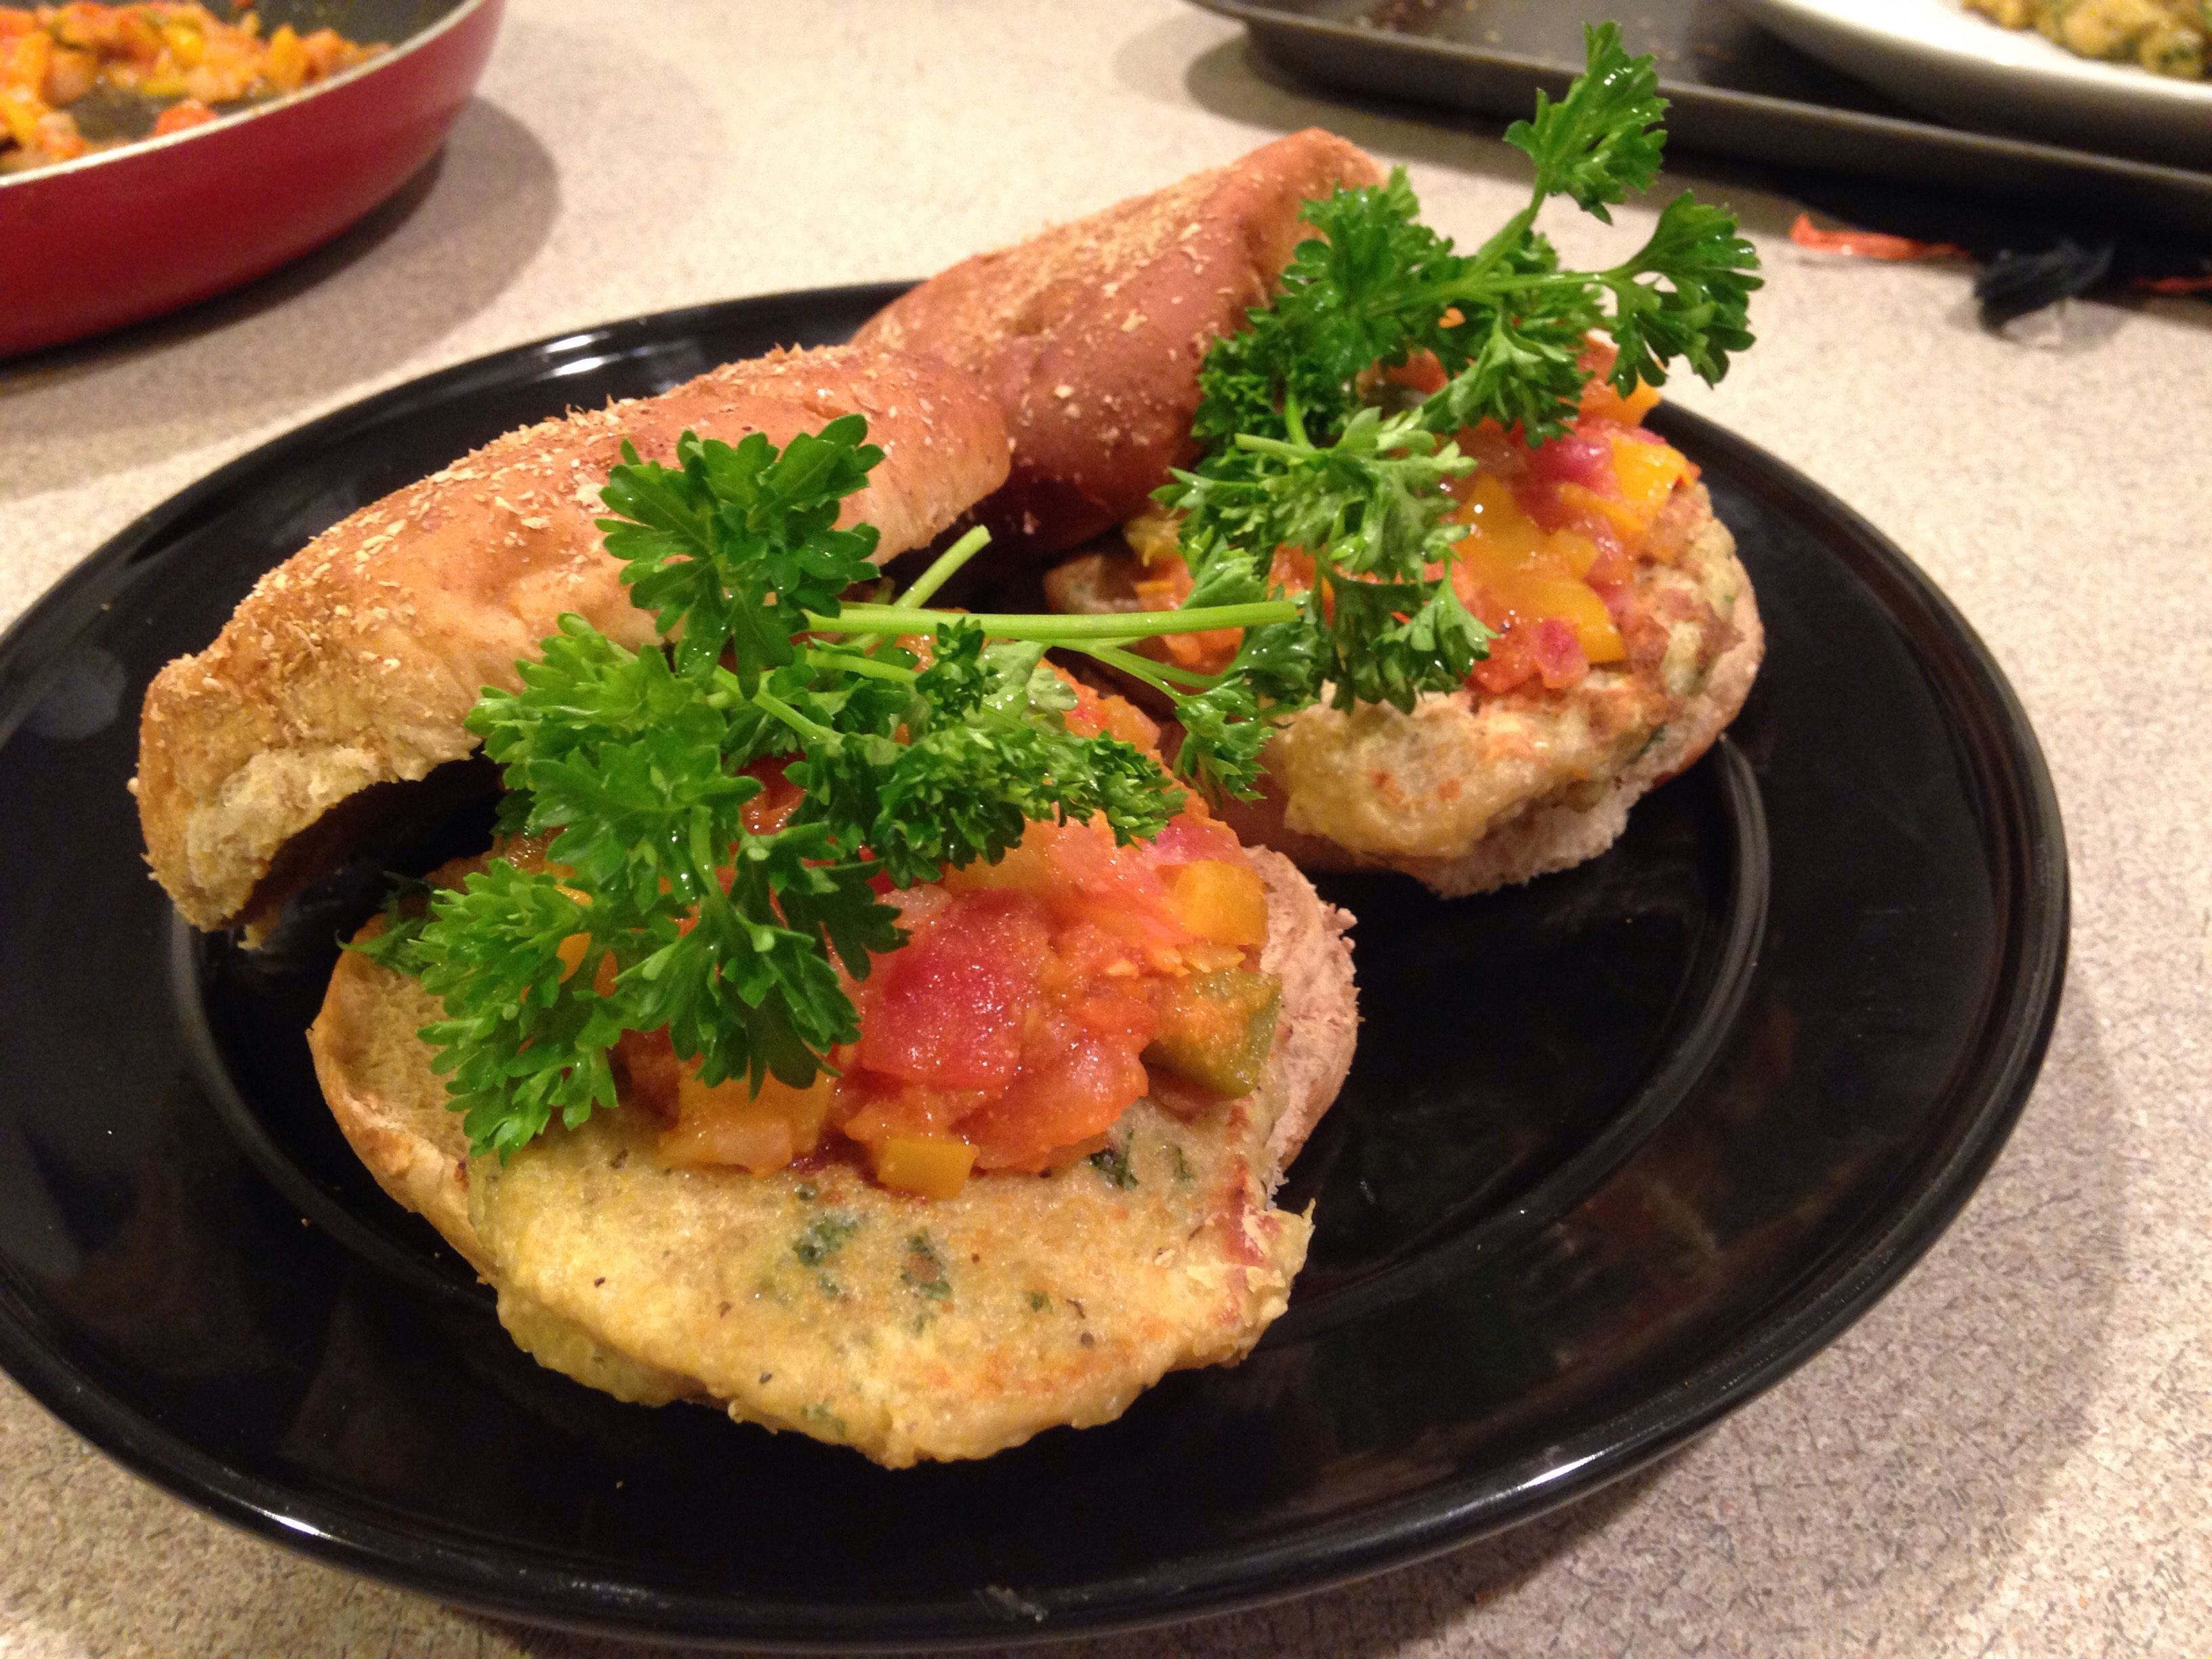
\includegraphics[height=\paperheight,%
				keepaspectratio]{./Images/QuinoaPatties.jpg}}%
			\vfill
}}}

%TITLE AND AUTHOR
\title{{\huge \textbf{The Antonius Cookbook} \\ \textbf{Version -- \Version}} \\ \vspace{1cm}
	%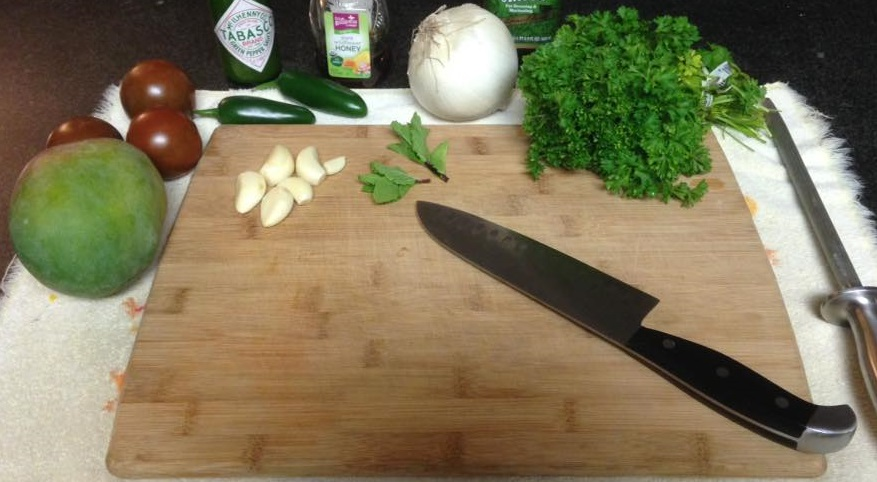
\includegraphics[scale =0.45]{./Images/CoverCropped.jpg}
}
\author{Written and Compiled by: Antonius Torode \\ Michigan State University \\ Department of Physics \& Astronomy}
\date{Latest update: \today}

\begin{document}
	
\AddToShipoutPicture*{\ChickenSalad}

%BEGIN FRONT MATTER
%\setlength{\parindent}{0pt}
\frontmatter
\clearpage
\maketitle
\pagestyle{empty}
\AddToShipoutPicture*{\TowerGarden}
%% copyrightpage
\begingroup
\footnotesize
\parindent 0pt
\parskip \baselineskip
\textcopyright{} 2017 Antonius Torode \\
All rights reserved.

This work may be distributed and/or modified under the conditions of Antonius’ General Purpose License (AGPL).

The Original Maintainer of this work is: Antonius Torode.

The Current Maintainer of this work is: Antonius Torode.

Primary Shareholder: Pranjal Tiwari

This document is designed for the purpose of storing and sharing recipes that have either been discovered by or created by myself (the author). All images are taken by myself of meals I have prepared unless otherwise stated.

\begin{center}
\begin{tabular}{ll}
Most Current Revision Date: &  \today 
\end{tabular}
\end{center}

Published by Antonius Torode. 

Hosted at: https://msu.edu/{\raise.17ex\hbox{$\scriptstyle\sim$}}torodean/ACookbook.html

Github Repository: https://github.com/torodean/Antonius-Cookbook

\vfill


Torode, A.\\
\hspace*{2em} The Antonius Cookbook \\
\hspace*{2em} Version -- \Version \\
\hspace*{2em} Michigan State University -- \\
\hspace*{2em} Department of Physics \& Astronomy. \\
\hspace*{2em} 2016, Student. \\
\hspace*{2em} ISBN: NONE \\



\endgroup
\clearpage
\tableofcontents
\newpage
\vspace*{\fill}
\begin{center}
	\textit{This page intentionally left blank. \\ (Yes, this is a contradiction.)}
\end{center}
\vspace*{\fill}

%BEGIN MAIN MATTER
\mainmatter
\pagestyle{fancy}

%BREAKFASTS
\AddToShipoutPicture*{\driedfruit}
\chapter{Breakfasts}

Breakfast is the first meal of the day and an important part of the day in that it proves you energy early in the morning after sleeping through the night. The word refers to breaking the fasting period of the previous night. Any foods can be eaten for breakfast, as with all meals, but it is important to have a nutrition packed meal to revitalize you for the day. Breakfast has been popularly refered to as ``the most important meal of the day'' in some areas. Some epidemiological studies even link an association between breakfast consumption and a lower risk of type two diabetes mellitus and metabolic syndrome\footnote{Maki KC, Phillips-Eakley AK, Smith KN (2016). "The Effects of Breakfast Consumption and Composition on Metabolic Wellness with a Focus on Carbohydrate Metabolism". Adv Nutr. 7 (3): 613S–21S. doi:10.3945/an.115.010314. PMID 27184288.}.
\thispagestyle{fancy}
\section{Egg Sandwich}
\AddToShipoutPicture*{\EggSandwich}

\subsection*{Base Ingredients}
\begin{multicols}{3}
	\begin{itemize}
		\item English Muffin or Toast
		\item 2-3 Eggs
		\item Beef Summer Sausage
		\item Butter
		\item Olive oil
		\item Milk
		\item Garlic
		\item Salt \& Pepper
	\end{itemize}
\end{multicols}
\subsection*{Spinach and Feta (optional)}
\begin{multicols}{3}
	\begin{itemize}
		\item Spinach
		\item Feta Cheese
		\item Onion
	\end{itemize}
\end{multicols}
\subsection*{Greek Delight (optional)}
\begin{multicols}{3}
	\begin{itemize}
		\item Mushroom
		\item Green Pepper
		\item Onion
		\item Tomato
		\item Ginger
		\item Fresh Parsley
	\end{itemize}
\end{multicols}

\subsection*{Your Favorite Omelet}
You can use ingredients of your liking. This is a very versatile dish.

\subsection*{Preparation}
Toast English muffin or bread to desired level while preparing other ingredients. Scramble eggs in a separate bowl with a small drizzle of milk (this helps them fluff up) and dice other optional ingredients. Slice Summer Sausage into circles and place in a medium-low heat pan. When the sausages start to bubble, they are ready to be flipped. While that is cooking, in a hot pan, lightly drizzle olive oil and place in Minced Garlic and other optional ingredients\footnote{If you are using greens such as spinach, parsley, cilantro, etc. or cheeses such as cheddar, swiss, feta, etc., wait to put these in until the eggs are in.}. Saut\`{e} these until they start browning. Once browning begins, add eggs\footnote{This is when it is a good idea to add items such as Parsley, Spinach, cheese, etc.}. Place lobs of butter on edges of omelet as it cooks. Once cooked, add Salt \& Pepper and remove from pan. 

When toast is finished, butter it. When sausage is finished, dab with paper towel to remove excess grease. Cut omelet in half or appropriate size for bread and assemble sandwich by bread|egg|sausage|bread. Enjoy with a side of fruit and a warm cup of tea for best breakfast results.


\subsection*{Tips}

Do not season the eggs before they are cooked. To practice flipping an omelet, you can get a piece of toast in an empty frying pan and flip it. A great way to slice spinach for use in something like this where you are not cooking it down for a while is to roll the leaves together and slice into strips (being careful not to crush the leaves). You can also make home made sausage with ground beef and the appropriate seasonings which will go brilliantly well as a replacement to any sausage. A small amount of fresh ginger is a great addition to most combinations of ingredients here. Cinnamon toast is also a great choice (and a childhood favorite of mine) for use with these sandwiches.
%\thispagestyle{fancy}
\section{Spinach and Feta Eggs}
\AddToShipoutPicture*{\FetaSpinachEggs}
%\thispagestyle{fancy}
\section{Venison and Eggs}
\AddToShipoutPicture*{\SteakAndEggs}

\subsection*{Ingredients}

%LUNCHES
\AddToShipoutPicture*{\SalmonVegetableRice}
\chapter{Lunches}

Lunch is an abbreviation of the word luncheon. It is a meal typically eaten around midday shortly after second breakfast, elevenses, and before afternoon tea (if you're a hobbit that is). The word luncheon is derived from nuncheon which means light snack\footnote{Dhirendra Verma (1999). Word Origins. Sterling Publishers Pvt. Ltd. p. 52. ISBN 978-81-207-1930-9. Retrieved March 15, 2016.}, and can range from a light snack to a large meal. Since it occurs around midday when many people are still at work, it is often accompanied with a social gathering in which conversing happens. For this reason, lunches are generally made to be quick, tasty so that as to elicit conversation and not take up a significant portion of the day.
\thispagestyle{fancy}
\section{Spicy Mexican Soup}
\AddToShipoutPicture*{\MexicanSoup}
This recipe was adapted from the youtube video ``Spicy Mexican Soup with Tortillas \& Salsa - Gordon Ramsay.'' I would highly recommend watching 
\subsection*{Ingredients}
\begin{multicols}{3}
	\begin{itemize}
		\item Red Onions
		\item Habanero (or chipotle)
		\item 1 Teaspoon Cumin seeds
		\item 1 Teaspoon Oregano
		\item 2 Clove Garlic
		\item Olive Oil
		\item 1 Tablespoom Brown Sugar
		\item 1 Tablespoon Tamato Puree
		\item 1 Tomato
		\item 1 Can of Kidney Beans
		\item 1 Orange Bell Pepper
		\item $\frac{1}{2}$-1 cup vegetable stock
		\item Cilantro or Coriander
	\end{itemize}
\end{multicols}

\subsection*{Preparation}

Begin by drizzling olive oil in a hit pot and add finely sliced red onions, Bell pepper and habanero. Add finely diced garlic, oregano and cumin seems and reduce down until ingredients brown. Drizzle olive oil again generously which will help reduce spice. Add brown sugar and coat ingredients in the light caramel. Add tomato puree and blend well. Add one whole diced tomato, kidney beans, and vegetable stock. Let simmer and stir occasionally. The longer you cook the dish the hotter (spicier) it will become. When done, add fresh cilantro or Coriander and mix in. 

This dish is well served with avocado and cheese or with a side of garlic bread. Garlic bread can be made simply by buttering your favorite bread, adding garlic powder and sea salt, and then baking until golden brown and crispy. 

\subsection*{Tips}

Habanero works well with this dish if you can handle a good deal of spice. If not, you may want to use something less potent like chipotle or chili peppers. You can also leave the spice out entirely but the flavor from the spice adds a lot to this dish.
\section{Mango Salsa Taco}
\AddToShipoutPicture*{\MangoSalsaTaco}
\thispagestyle{fancy}
\section{Vegetable Stir Fry With Rice Noodles}
\AddToShipoutPicture*{\StirFryRiceNoodles}

\subsection*{Ingredients}
\begin{multicols}{3}
	\begin{itemize}
		\item 
	\end{itemize}
\end{multicols}
\thispagestyle{fancy}
\section{Steak Sandwich with Tomato Relish} \label{SteakSandwich}
\AddToShipoutPicture*{\SteakSandwich}

This recipe was adapted from Gordon Ramsay's "The Ultimate Steak Sandwich" found on YouTube. I would recommend watching the video to see it prepared.

\subsection*{Ingredients}

\begin{multicols}{3}
	\begin{itemize}
		\item Fillet Mignon
		\item Fresh Thyme
		\item Butter
		\item 1 Clove Garlic
		\item $\frac{1}{2}$ Red Onion
		\item $\frac{1}{2}$ Red Bell Pepper
		\item 1 cup Cherry Tomatoes
		\item 1 Large Jalape\~{n}o
		\item Fresh Basil
		\item Apple Cider Vinegar
		\item Olive Oil
		\item Romaine Lettuce
		\item Stone Ground Mustard
		\item Mayonnaise
		\item Salt \& Pepper
		\item French Bread
	\end{itemize}
\end{multicols}

\subsection*{Preparation}
Pre-heat oven to $190^\circ C$ ($375^\circ F$)  In a hot pan, lightly drizzle olive oil and sear fillet on all sides. Lightly butter the fillet quickly or place small slabs of butter on top. Slice garlic clove into two pieces through the side and place them into pan with thyme on top. Use this as a bed to place fillet on top of and cook in oven for 10-15 minutes. When finished, let the fillet rest for 10 minutes and baste with juices from cooking.

In a separate hot pan, generously drizzle olive oil and add finely diced onions, bell pepper, and Jalape\~{n}o. Slice tomatoes in half and place them in pan as well. As the tomatoes heat up crush with a spoon. Add about a tablespoon on vinegar and cook until the mixture is no longer sour. Lightly slice basil leaves and add to completed mixture when desired consistency is met. 

To prepare sandwich, drizzle olive oil on sliced french bread and grill in pan until lightly charred (or to desired texture) on both sides. Slice fillet into strips. Mix in a small bowl 1 part mustard and 1 part mayonnaise and place on bread, followed by lettuce, fillet, relish and then topped with bread. Slice in half and enjoy!

\subsection*{Tips}
When slicing hte fillet, keep the pieces thick so that they retain their heat longer. Even to people who do not like either mayonnaise or mustard, mixing the two as described above gives a unique condiment unlike either individually. I have had personal experience with someone who did not like either on their own but liked the combination of the two. Be sure to cook the relish long enough after adding the vinegar so that the dish does not taste sour. Always taste ones cooking until it is as desired.
\thispagestyle{fancy}
\section{Fresh and Simple Pizza}
\AddToShipoutPicture*{\Pizza}

\subsection*{Ingredients}

%DINNERS
\AddToShipoutPicture*{\Steak}
\chapter{Dinners}

Dinner generally refers to the largest meal of the day in many English-speaking cultures. The word comes partially from an Old French word ``disner'' which means to ``dine'', combined with some Latin etymology\footnote{Etymology of "dinner" from Online Dictionary. Accessed November 11, 2009.}. In many parts of the world and even between many families, dinner falls within vastly different times of the day. Some prefer an early dinner shortly after midday while others prefer dinners late into the evening. Regardless of the time of day, dinner is generally the meal that would require the most amount of time to prepare compared to others as it generally falls after ones work day or even as a closing to it.

\section*{Tips to a Healthy Dinner}
\begin{enumerate}
	\item Use fresh ingredients.
	\item Eat a variety of food.
	\item Eat smaller portions and stop eating when you are not hungry (don't over eat).
	\item Avoid products with a lot of ingredients to make your food simple!
	\item Don't cook with fatty meats. A lean piece of meat can contain as much if not more flavor than a fatty one if cooked and seasoned properly.
\end{enumerate}
\thispagestyle{fancy}
\section{Calzone}
\AddToShipoutPicture*{\Calzone}

\subsection*{Ingredients}
\thispagestyle{fancy}
\section{Alfredo}
\AddToShipoutPicture*{\Alfredo}

\subsection*{Ingredients}
\begin{multicols}{3}
	\begin{itemize}
		\item 
	\end{itemize}
\end{multicols}
\thispagestyle{fancy}
\section{Marinated Chicken And Vegetables on a Bed of Rice}
\AddToShipoutPicture*{\MarinatedChickenAndRice}
\thispagestyle{fancy}
\section{Ground Beef Lasagna}
\AddToShipoutPicture*{\Lasagna}

\subsection*{Ingredients}
\begin{multicols}{3}
	\begin{itemize}
		\item 
	\end{itemize}
\end{multicols}
\thispagestyle{fancy}
\section{Venison with Homemade Barbecue Sauce}
\AddToShipoutPicture*{\VenisonBBQ}

\subsection*{Ingredients}
\begin{multicols}{3}
	\begin{itemize}
		\item Small Tomato's
		\item Mushrooms
		\item Venison
		\item Olive Oil
		\item Salt \& Pepper
		\item 2 Tablespoons Butter
		\item Garlic
	\end{itemize}
\end{multicols}

\subsection*{Barbeque Sauce}
This Barbeque Sauce Recipe is derived from the YouTube video "Smoky Pork Sliders with BBQ Sauce - Gordon Ramsay." I would highly recommend watching it to see how it is cooked.
\begin{multicols}{3}
	\begin{itemize}
		\item 1 Onion
		\item 3 Cloves Garlic
		\item 2 Teaspoons Olive Oil
		\item 1 Tablespoon Brown Sugar
		\item 1 Teaspoon Smoked Paprika
		\item 1 Tablespoon Ketchup
		\item 2 Tablespoons Apple Cider Vinegar
	\end{itemize}
\end{multicols}

\subsection*{Preparation}
\textbf{Barbecue Sauce:} In a hot pan, drizzle olive oil and add finely diced garlic and onions. Saut\'{e} until browning then add brown sugar and caramelize. Add smoked paprika, mix well and then add vinegar. Reduce mixture to remove sourness from vinegar. Once reduced fully, add ketchup and cook until desired thickness is reached.

\vspace{0.25cm}

\textbf{Venison:} Preheat oven to $205^\circ$C (400$^\circ$F). Season Venison generously with salt \& Pepper. In a hot pan, drizzle olive oil. Seer venison on all sides then melt butter over top. Add peeled Garlic cloves to pan and set venison onto garlic so it is not touching the pan (This will help it cook evenly in the oven). Place in oven and let cook for 12-15 minutes\footnote{Time to cook heavily depends on size and shape of meat.} or to desired wellness. In a small pan on low heat, drizzle olive oil and add tomatoes and mushrooms (bulb side down). Season tomatoes and mushrooms and let cook until soft and wrinkled. After venison is cooked, baste with butter and remove from pan. Let venison rest for 10 minutes before cutting (It will continue to cook slightly during this process).

\subsection*{Tips}

In the original recipe, Worcestershire sauce is added with the ketchup to add extra flavor. When cooking tomatoes slowly like we are in this recipe, it is helpful to buy tomatoes still on the vine that way we can set them into the pan with the stem and remove them the same way. It also holds them together which makes for easy plating. It is a good idea to always poke meat when cooking with two fingers. Depending on the meat and firmness of it when touching, this can give you a very good idea of how cooked it is (This comes with practice).

%SNACKS
\AddToShipoutPicture*{\FruitBowl}
\chapter{Snacks, Sides \& Toppings}

A snack is a portion of food that is too small to consider a full meal. A side is essentially a snack that goes with a meal. A topping is meant to be served with a meal. Snacks are generally eaten between meals while sides and toppings are served either with a meal or with a snack. Snacks are typically prepared with ingredients commonly available for those times where you are not ready to prepare a planned meal but you are still hungry. Many of todays commercially available snacks are high in sugars and fats but are packed with flavor which are typically eaten due to a craving or to hold one over until the next meal. They are popular because they are usually sold in vending machines and easily accessible or store-able A much better snack by far is any combination of whole foods which include fruits, vegetables, nuts and berries which can serve as an excellent source of nutrition between meals when one finds them self in need of food. 


\section*{Tips to a Healthy Snack}
\begin{enumerate}
	\item Avoid processed snacks like potato chips or snack bars.
	\item Avoid sugary snacks.
	\item Grab a piece of fruit.
	\item Grab some vegetables.
	\item Grab some assorted trail mix with dried fruits.
	\item Fruits and vegetables are perfect for snacks because they contain a balance of vitamins, minerals, fiber, and more. This will leave you will energy and nutrients for the remainder of the day.
\end{enumerate}
\thispagestyle{fancy}
\section{Fruit Medley}
\AddToShipoutPicture*{\FruitMedley}
\thispagestyle{fancy}
\section{Lemon Poppyseed Muffins}
\AddToShipoutPicture*{\LemonPoppyseed}

\subsection*{Ingredients}
\thispagestyle{fancy}
\section{Tortilla Chips}
\AddToShipoutPicture*{\TortillaChips}

\subsection*{Ingredients}
\begin{multicols}{3}
	\begin{itemize}
		\item Tortilla's
		\item Olive Oil
		\item Paprika
		\item Lime
	\end{itemize}
\end{multicols}

\subsection*{Preparation}

Pre-heat oven to $190^\circ C$ ($375^\circ F$). Lightly coat tortillas in olive oil and sprinkle with paprika. Rub paprika into tortillas. Cut tortillas into desired chip shape and place on a large baking sheet and place in oven until chips are crispy. Squeeze lime juice over chips and enjoy!

\subsection*{Tips}

Depending on the type of tortilla's used, the cooking time on this will vary.
\vspace{2cm}
\section{Mexican Spinach Dip}

This recipe was originally introduced to me by Mariah Fitch.
\subsection*{Ingredients}
\begin{multicols}{3}
	\begin{itemize}
		\item 1 Jar salsa
		\item 10 Oz. Spinach
		\item 2 Cups Shredded Cheese
		\item 1 8 Oz. packages of Cream Cheese
		\item 1 Cup Evaporated Milk
		\item 2.25 Oz. Olives
		\item 1 Tablespoon Red Wine Vinegar
		\item Salt \& Pepper
	\end{itemize}
\end{multicols}

\subsection*{Preparation}

Combine ingredients into large bowl and mix well. Serve with Favorite chips.
\thispagestyle{fancy}
\section{Mango Salsa}
\AddToShipoutPicture*{\MangoSalsa}
\thispagestyle{fancy}
\section{Strawberry Pecan Side Salad}
\AddToShipoutPicture*{\StrawberrySalad}

\subsection*{Salad Ingredients}

\begin{multicols}{3}
	\begin{itemize}
		\item Mixed Greens
		\item Pecans
		\item Strawberries
		\item Raisins
		\item Hemp Seeds
	\end{itemize}
\end{multicols}

\subsubsection*{Dressing Ingredients}
This is a very simple and versatile dressing that goes great on many dishes and salads.
\begin{multicols}{3}
	\begin{itemize}
		\item 1 Part Fresh Lemon Juice
		\item 2 Part Filtered Water
		\item 2 Part Olive Oil
		\item Salt \& Pepper (lightly)
	\end{itemize}
\end{multicols}

\subsection*{Preparation}

Combine Salad ingredients into large bowl. Combine dressing ingredients into a dressing bottle and shake well. Drizzle dressing over salad and serve.

%DESSERTS
\AddToShipoutPicture*{\AppleTartLarge}
\chapter{Desserts \& Sweets}
\thispagestyle{fancy}
\section{New York Cheesecake}
\AddToShipoutPicture*{\Cheesecake}

\subsection*{Ingredients}
\begin{multicols}{2}
	\begin{itemize}
		\item 3 8 Oz. packages of Cream cheese
		\item 3 Eggs
		\item 2 Tablespoons Flour
		\item 1 Cup Cane Sugar
		\item 1 Large Lemon
	\end{itemize}
\end{multicols}

\subsection*{Preparation}
Preheat oven to $180^\circ C$ ($355^\circ F$). In a large Bowl, whisk cream cheese and sugar together until they are well blended and very soft. In a separate bowl, whisk 3 eggs together. Add the eggs to the cream cheese mixture one third at a time and whisk well after each addition. Once all of the eggs are in the mixture, add 2 tablespoons of flour and again blend well. Finish mixture off with the zest of a whole large lemon. For extra lemon flavor a small squeeze of lemon juice can be added as well. Pour the mixture into a buttered cheesecake pan. Gently tap the pan on a surface so that all of the gaps between the pan and mixture are filled. Bake in oven for 35-40 minutes.

\subsection*{Tips}
It will be much easier to mix the cream cheese if left out of the fridge for about 15 minutes before use.

\subsection*{Additions - Marble}
Although this recipe is great on its own, it is great served with raspberries or strawberries. One can also add a marble to the cheesecake using some Cherry Tart Concentrate. To do this, once the mixture is in the pan, pour a small amount of cherry concentrate over the center and swirl into the mixture with a large whisk.


\thispagestyle{fancy}
\section{Warm Apple Tart With Ice Cream} \label{appletart}
\AddToShipoutPicture*{\AppleTart}

The background image of this apple tart was taken by Samantha Murray. This recipe was originally one of Gordon Ramsay's and modified from there.

\subsection*{Ingredients}
\begin{multicols}{3}
	\begin{itemize}
		\item Puff Pastry
		\item Honey Crisp apples
		\item Cane Sugar
		\item Butter
		\item Powdered Sugar
		\item Favorite Ice Cream
		\item Chocolate Ganache
	\end{itemize}
\end{multicols}

\subsection*{Preparation}

Pre-heat Oven to $190^\circ C$ ($375^\circ$ F). On a large sheet of Parchment paper, roll out puff pastry and cut into desired shape. Gently poke the puff pastry with a fork so that it has holes in various places (this keeps it from bubbling up while cooking). Thinly slice cored and peeled apples and lay atop the pastry overlapping each other so that the pastry is covered. Brush top with melted butter and sprinkle cane sugar over top pastry to cover apples. Place in oven to caramelize and until apples are tender and pastry is golden (about 25-30 minutes). Once finished, lightly sift powdered sugar over top and caramelize with blow-torch and serve Warm with a scoop of Vanilla or your favorite ice cream. For extra finesse, make a chocolate ganache to drizzle over top which can be found in section \ref{ganache}.

\subsection*{Tips}

Puff Pastry can be bought in store but it is hard to find a good puff pastry using good ingredients. If you are bold you can make your own, but I buy mine from Whole Foods which uses great ingredients and works well with this recipe. When baking this, it is best to use a pan with edges on it in case the caramelized sugar runs off of the edge. My favorite combination to use with this is a black cherry ice cream with a dark chocolate ganache found in section \ref{ganache}.
\thispagestyle{fancy}
\section{Chocolate Ganache} \label{ganache}
\AddToShipoutPicture*{\Strawberries}

\subsection*{Ingredients}
\begin{multicols}{3}
	\begin{itemize}
		\item 1 70\% Dark Chocolate Bar
		\item 1 Tablespoon Butter
		\item 1 Tablespoon Honey
		\item $\frac{1}{2}$ Cup Heavy Cream
	\end{itemize}
\end{multicols}

\subsection*{Preparation}

In a pot, warm the cream to just before a boil. Dice the chocolate into small pieces and place in bowl with butter and honey. Once cream is warm pour into chocolate mixture and gently mix with a spoon until blended. Let cool for 5-10 minutes and then mix well with a whisk to allow the mixture to aerate. This can be served as a warm topping or cooled and used as a fruit topping. Depending on the intended use, you may want to cool this for a short amount of time. My favorite use of this is in conjunction with the warm apple tart found in \ref{appletart}.

\subsection*{Tips}

The better the chocolate, the better the ganache.
\thispagestyle{fancy}
\section{Saffron Cardamom Ice Cream}
\AddToShipoutPicture*{\SaffronIceCream}

\subsection*{Ingredients}
This recipe was based off of and modified from "Saffron Cardamom Ice Cream With Pistachios" found on www.food.com and introduced to me by Pranjal Tiwari.
\begin{multicols}{3}
	\begin{itemize}
		\item 2 Cups Milk
		\item 2 Cups Heavy Cream
		\item $\frac{1}{4}$ Teaspoon Saffron Thread
		\item 8 Large Egg Yolks
		\item $\frac{3}{4}$ Cup Cane Sugar
		\item 2 Teaspoons Ground Cardamom
	\end{itemize}
\end{multicols}

\subsection*{Preparation}

Using a Pestal, finely ground saffron and add to cream and milk in a saucepan. Bring to boil. Remove pan from heat and let stand covered for 1 hour. Return pan to heat and bring the mixture to a simmer. In a separate bowl, mix egg yolks, salt and sugar together well so that they have a custard texture. Add half a cup of cream mixture into custard and mix well. Then mix rest of cream mixture in slowly while mixing. Place mixture back into saucepan and cook over medium-low heat while stirring until reaching $75^\circ$ C ($170^\circ$ F). Strain mixture through a fine sieve and add cardamom. Stir well and place pan in cold water to chill. Once cooled off, place in freezer. Every 25 minutes, stir to prevent water crystals from forming. Once too thick to stir, cover and let freeze.
\thispagestyle{fancy}
\section{Cheesecake Topping}
\AddToShipoutPicture*{\CheesecakeTopping}

\subsection*{Ingredients}
\begin{multicols}{3}
	\begin{itemize}
		\item Strawberries
		\item Blueberries
		\item Cane Sugar
		\item Creme De Casis
	\end{itemize}
\end{multicols}

\subsection*{Preparation}

Wash strawberries and blueberries well before hand and allow to fully dry before using. In a hot pan, pour cane sugar to cover bottom of pan. Slice strawberries in half (thirds for large ones) Let sugar Melt into caramel. Place strawberries and blueberries into pan with caramel and toss to coat fruit. Deglaze pan with Creme De Casis and set to side to cool for a few minutes.

%BEGIN BACKMATTER
\backmatter
% bibliography, glossary and index would go here.

\end{document}